\documentclass[12pt,a4paper]{article}

\usepackage{michel}
\usepackage[dcucite,abbr]{harvard}
\harvardparenthesis{none}\harvardyearparenthesis{round}
\usepackage{hyperref}
\usepackage{longtable}

\title{Estimating choice models with latent variables with Biogeme}
\author{Michel Bierlaire \and Moshe Ben-Akiva \and Joan Walker} 
\date{\today}


\begin{document}


\begin{titlepage}
\pagestyle{empty}

\maketitle
\vspace{2cm}

\begin{center}
\small Report TRANSP-OR xxxxxx  \\ Transport and Mobility Laboratory \\ School of Architecture, Civil and Environmental Engineering \\ Ecole Polytechnique F\'ed\'erale de Lausanne \\ \verb+transp-or.epfl.ch+
\begin{center}
\textsc{Series on Biogeme}
\end{center}
\end{center}


\clearpage
\end{titlepage}


The package Biogeme (\texttt{biogeme.epfl.ch}) is designed to estimate
the parameters of various models using maximum likelihood
estimation. It is particularly designed for discrete choice
models.  In this document, we present how to estimate choice
models involving latent variables.

We assume that the reader is already familiar with discrete choice
models, and has successfully installed Biogeme. This document has
been written using Biogeme 3.3.



\section{Models and notations}

The literature on discrete choice models with latent variables is vast
(\cite{walker2001extended}, \cite{ashok2002extending},
\cite{greene2003latent}, \cite{ben2002integration}, to cite just a
few). We start this document by a short introduction to the models and
the notations. 

A \emph{latent variable} is a variable that cannot be directly
observed. It is typically modeled using a \textbf{structural
  equation}, which expresses the latent variable as a function of
observed (explanatory) variables and an error term. A general form of
such a structural equation is:
\begin{equation}
\label{eq:structural}
x_{nk}^* = x^*(x_n; \psi_k) + \omega_{nk},
\end{equation}
where $n$ indexes individuals, $x_{nk}^*$ is the $k$th latent variable of interest, $x_n$ is a vector of observed explanatory variables, $\psi_k$ is a vector of parameters to be estimated, and $\omega_{nk}$ is a stochastic error term, normally distributed $N(0, \Sigma_{\omega k})$, where $\Sigma_{\omega k}$ is the variance-covariance matrix.

A common specification assumes a linear functional form  i.i.d.   error terms:
\begin{equation}
\label{eq:linearStructural}
 x_{nk}^* = \psi_{0k} + \sum_s \psi_{sk} x_{ns} + \sigma_{\omega k} \omega_{nk},
\end{equation}
where $\omega_{nk} \sim N(0, 1)$, $\psi_{0k}$ is an intercept term, and $\sigma_{\omega k}$ is a scaling parameter for the error term. The vector $\sigma_\omega = (\sigma_{\omega 1}, \ldots, \sigma_{\omega K})^\top$ corresponds to the diagonal of the covariance matrix $\Sigma_{\omega n}$, with all off-diagonal elements set to zero, implying uncorrelated errors across alternatives.

In discrete choice models, for example, the utility $U_{in}$ that
individual $n$ associates with alternative $i$ is a typical example of
a latent variable.

Information about latent variables is obtained indirectly through
\emph{measurements}, which are observable manifestations of the
underlying latent constructs. For example, in discrete choice models,
utility is not directly observed but is inferred from the choices
individuals make. The relationship between a latent variable and its
associated measurements is described by \textbf{measurement
  equations}. The specific form of these equations depends on the
nature of the observed measurements (e.g., continuous, or ordinal).


\subsection{Measurement equations: the continuous case}

Since latent variables cannot be directly observed, analysts rely on
indirect measurements to infer their values. A common approach
involves asking respondents to rate the perceived magnitude of the
latent construct on an arbitrary scale. For example: \emph{``How would
you rate the level of pain that you are experiencing, from 0 (no pain)
to 10 (worst pain imaginable)?''}

Each such rating is referred to as an \emph{indicator}, indexed by
$\ell=1, \ldots, L_n$, and is modeled using a \textbf{measurement equation}. This
equation relates the observed indicator to the latent variables and
other explanatory variables:
\begin{equation}
\label{eq:continuousMeasurement}
I_{n\ell} = I_\ell(x_n, x_n^*;\lambda_\ell) + \upsilon_{n\ell}, \; \forall \ell=1, \ldots, L_n, \forall n,
\end{equation}
where $I_{n\ell}$ denotes the response provided by individual $n$ for
indicator $\ell$, $x_n^*$ is the latent variable of interest (e.g., pain
perception), $x_n$ is a vector of observed explanatory variables (such as
socio-demographic characteristics), $\lambda_\ell$ is a vector of $K^\lambda$
parameters to be estimated, and $\upsilon_{n\ell}$ is a normally distributed random error term with mean 0 and variance-covariance matrix $\Sigma_{\upsilon \ell}$. 

A common specification of the measurement function assumes linearity
and normally distributed errors:
\begin{equation}
\label{eq:linearMeasurement}
I_{n\ell} = \sum_k \lambda_{\ell k}  x_{nk}^* + \sum_{s} \lambda_{\ell s} x_{ns} + \sigma_{\upsilon \ell} \upsilon_{n\ell}, \quad \forall \ell,
\end{equation}
where $\lambda_{\ell k}$ are unknown parameters to be estimated, $\sigma_{\upsilon \ell}$ is an indicator-specific scale parameter, and $\upsilon_{n\ell} \sim N(0, 1)$.


\subsection{Measurement equation: the ordinal case}

Another type of indicator arises when respondents are asked to
evaluate a statement using an ordinal scale. A typical context for
this type of measurement is the use of a Likert scale
(\cite{likert1932technique}), where individuals express their degree of
agreement or disagreement with a given statement. For example:
\begin{quote}
\emph{``I believe that my own actions have an impact on the planet.''} \\
Response options: strongly agree (2), agree (1), neutral (0), disagree ($-1$), strongly disagree ($-2$).
\end{quote}

Another common example is the observed choice itself. In discrete
choice models, whether or not an alternative is chosen is represented
by a binary variable, which can be interpreted as a special case of an
ordinal scale with only two categories.

To model these types of indicators, we represent the observed
measurement as an \emph{ordered discrete variable} $I_{n\ell}$, which
takes values in a finite, ordered set $\{j_1, j_2, \ldots, j_{M_\ell}\}$. The
measurement equation involves two stages:

\paragraph{Step 1: Latent response formulation.} We first define a continuous response variable, that happens to be unobserved (latent) in this case:
\begin{equation}
I^*_{n\ell} = I^*_\ell(x_n, x_n^*; \lambda_\ell) + \upsilon_{n\ell},
\end{equation}
where $I^*_{n\ell}$ is a continuous latent variable underlying the
reported response, $x_n^*$ is the relevant latent variable (e.g.,
environmental concern), $x_n$ is a vector of observed explanatory
variables (e.g., age, income), $\lambda$ is a vector of parameters to
be estimated, and $\upsilon_{n\ell}$ is a random error term.

\paragraph{Step 2: Discretization via thresholds.} Since $I^*_{n\ell}$ is not observed, we relate it to the reported discrete measurement $I_{n\ell}$ through a set of threshold parameters:
\begin{equation}
\label{eq:discreteMeas-b}
I_{n\ell} = \left\{
\begin{array}{ll}
j_1 & \text{if } I^*_{n\ell} < \tau_1, \\
j_2 & \text{if } \tau_1 \leq I^*_{n\ell} < \tau_2, \\
\vdots \\
j_m & \text{if } \tau_{m-1} \leq I^*_{n\ell} < \tau_m, \\
\vdots \\
j_M & \text{if } \tau_{M_\ell-1} \leq I^*_{n\ell},
\end{array}
\right.
\end{equation}
where $\tau_1, \ldots, \tau_{M_\ell-1}$ are threshold parameters to be estimated, satisfying the ordering constraint:
\begin{equation}
\label{eq:discreteMeas-c}
\tau_1 \leq \tau_2 \leq \cdots \leq \tau_{M_\ell-1}.
\end{equation}
Note that it is customary to use the same set of parameters for all
individuals $n$ and all indicators $\ell$, which explains the absence
of these indices on the parameter $\tau$.

Defining $\tau_0=-\infty$ and $\tau_{M_\ell}=+\infty$, it simplifies to
\begin{equation}
I_{n\ell} = j_m  \text{ if } \tau_{m-1} \leq I^*_{n\ell} < \tau_m, \; m=1, \ldots, M_\ell. 
\end{equation}






\subsection{Summary of notations}

\begin{longtable}{lp{6cm}l}
$n$           & index for individuals         & $\mathbb{N}$ \\
$N$           & number of individuals in the sample & $\mathbb{N}$\\
$\C$          & universal choice set        &    \\
$\C_n$        & choice set of individual $n$ \\
$i,j \in \C_n$  & indices of  alternatives \\
$J$           & total number of alternatives in $\C$ & $\mathbb{N}_0$  \\
  $J_n$         & number of alternatives in $\C_n$ & $\mathbb{N}$ \\
  $L_n$   & number of indicators available for individal $n$ & $\mathbb{N}$ \\
  $M_\ell$ & number of levels for the discrete Likert scale of indicator $\ell$ & $\mathbb{N}$ \\
$\theta=(\theta_1,\ldots,\theta_{K^{\theta}})^T$      & vector of all unknown
parameters  & $\R^{K^{\theta}}$  \\
$\beta=(\beta_1,\ldots,\beta_K)^T$      & vector of  unknown
coefficients in the systematic part
of the utility& $\R^K$  \\
$\gamma=(\gamma_1,\ldots,\gamma_{K^{\gamma}})^T$ & vector of unknown parameters that are not coefficients  & $\R^{K^{\gamma}}$ \\
$\alpha=(\alpha_1,\ldots,\alpha_{K^{\alpha}})^T$ & vector of all unknown parameters of structural equations & $\R^{K^{\alpha}}$ \\
$\psi=(\psi_1,\ldots,\psi_{K^{\psi}})^T$ & vector of  unknown coefficients in the systematic part  of the structural equations & $\R^{K^{\alpha}}$ \\
$\kappa=(\kappa_1,\ldots,\kappa_{K^{\kappa}})^T$ & vector of all unknown parameters of measurement equations & $\R^{K^{\alpha}}$ \\
$\lambda=(\lambda_1,\ldots,\lambda_{K^{\lambda}})^T$ & vector of unknown coefficients in the systematic part of measurement equations & $\R^{K^{\lambda}}$ \\
$m=(m_1,\ldots,m_{K^{m}})^T$ & vector of measurements/indicators & $\R^{K^{m}}$ \\
$S_n$ & vector of characteristics of individual $n$ or the choice context &
\\
$z_{in}$ & vector of attributes describing alternative $i$ as
perceived by individual $n$ \\
$x_{in} = (x_{in1},\ldots,x_{in{K^x}})^T$ & vector of explanatory
variables for alternative $i$ and individual $n$,  function of   attributes and 
characteristics, that is $x_{in}=h(z_{in},S_n)$ (for notational simplification, $K^x$ may be denoted by $K$ or $L$ in the text) & $\R^{K^x}$\\
$x^*_{n} = (x_{n1},\ldots,x_{n{K^{x^*}}})^T$ & vector of latent variables for individual $n$ & $\R^{K^{x^*}}$\\
$\varepsilon_{n}$ & vector of error terms of the utility functions  & $\R$ \\
$\omega_n$ & vector of error terms of structural equations  \\
$\upsilon_n$ & vector of error terms of measurement equations \\
$\LL^*(\theta)$      & likelihood function & $\R^{K^{\theta}}\rightarrow \R$ \\
$\LL(\theta)$      & log-likelihood function, $\LL(\theta) = \ln \LL^*(\theta)$ & $\R^{K^{\theta}}\rightarrow \R$,
 \\
$f_\varepsilon(\cdot;\theta)$ & probability density function (pdf)  of
continuous  random variable $\varepsilon$, parameterized by the vector $\theta$ & $\R^{K^{\varepsilon}}
\rightarrow \R^+$ \\
$F_\varepsilon(\cdot; \theta)$ & cumulative distribution function (CDF) of
random variable $\varepsilon$, parameterized by $\theta$  & $\R^{K^{\varepsilon}}
\rightarrow [0,1]$ \\
$\phi(\cdot)$ & probability density function of the univariate  standardized normal distribution & $\R
\rightarrow \R^+$ \\
$\Phi(\cdot)$ & cumulative distribution function of the univariate standardized normal distribution  & $\R
\rightarrow [0,1]$ \\
$R$ & number of draws in simulation context &  $\N$\\
$r$ & index of the draws in simulation context & $\N$ \\
$\Sigma_\xi$ & variance-covariance matrix of the normal random vector $\xi$ &$\R^{K^{\xi}\times K^{\xi}}$\\
\end{longtable}

\section{The MIMIC model}

The Multiple Indicators Multiple Causes (MIMIC) model is a structural
equation modeling framework designed to analyze relationships
involving latent variables. In a MIMIC model, the latent variable is
simultaneously influenced by a set of observed explanatory variables
(the ``multiple causes'') and reflected in several observed indicators
(the ``multiple indicators''). This dual structure enables the analyst
to capture both the determinants and the manifestations of latent
constructs, such as attitudes, preferences, or psychological traits.
A seminal introduction to the MIMIC model is provided by
\citeasnoun{Joreskog:1975aa}, who formalized its use within the
broader class of structural equation models.

The model involves the structural equations \req{eq:structural} and the measurement equations \req{eq:continuousMeasurement} and \req{eq:discreteMeas-b}. Conditional on the latent variables, the contribution of each indicator $\ell$ for each observation $n$ to the likelihood function is defined as follows.

\begin{equation}
  \label{eq:discreteMeas-d}
  \begin{aligned}
    \prob(I_{n\ell} = j_m| x^*_n, x_n ; \lambda_\ell, \Sigma_{\upsilon \ell}) &= \prob(\tau_{m-1} < I^*_{n\ell} \leq \tau_m) \\
    &= \prob(I^*_{n\ell} \leq \tau_m) -  \prob(I^*_{n\ell} \leq \tau_{m-1}),
  \end{aligned}
\end{equation}
where $j_m$ category $j_m$ observed  is then given by:

We can assume a linear specification of the latent response function, as in
Equation~\eqref{eq:linearMeasurement}:
\begin{equation}
  \label{eq:measurement_latent}
I^*_{n\ell} = \sum_k \lambda_{\ell k}  x_{nk}^* + \sum_{s} \lambda_{\ell s} x_{ns} + \sigma_{\upsilon \ell} \upsilon_{n\ell}, \quad \forall j,
\end{equation}
where the error term $\upsilon_{n\ell} \sim N(0,1)$. Using \req{eq:linearStructural}, we obtain
\begin{align*}
  I^*_{n\ell} &= \sum_k \lambda_{\ell k}  x_{nk}^* + \sum_{s} \lambda_{\ell k} x_{ns} + \sigma_{\upsilon \ell} \upsilon_{n\ell} \\
  &= \sum_k \lambda_{\ell k}  \psi_{0k} + \sum_{k} \lambda_{\ell k} \sum_s \psi_{sk} x_{ns} + \sum_k \lambda_k \sigma_{\omega k} \omega_{nk} + \sum_{s} \lambda_{\ell s} x_{ns} + \sigma_{\upsilon \ell} \upsilon_{n\ell} \\
\end{align*}
Clearly, the parameters of the structural and the measurement equations are confounded. The equation can be written
\begin{equation}
I^*_{n\ell} = \lambda'_{\ell 0} + \sum_s \lambda'_{\ell s} x_{ns} + \sigma'_{\upsilon\ell} \upsilon'_{n \ell},
\end{equation}
where $\lambda'_{\ell 0} =\sum_k \lambda_{\ell k}  \psi_{0k}$ is the intercept, $\lambda'_{\ell s} =\sum_{k} \lambda_{\ell k} \psi_{sk}+\lambda_{\ell s}$ are the coefficients of the socio-economic characteristics, $\sigma'_{\ell}=\sqrt{(\sum_k \lambda_k \sigma_{\omega k})^2+\sigma^2_{\upsilon \ell}}$ is the scale parameters, and $\upsilon'_{n \ell}\sim N(0,1)$. 


The
probability of observing category $j_i$ for individual $n$ and indicator $\ell$ becomes:
\[
\renewcommand{\arraystretch}{1.5}
\begin{array}{rcl}
\prob(I_{n\ell} = j_m| x^*_n, x_n ; \lambda_\ell, \Sigma_{\upsilon \ell}) &=&\prob(I_{n\ell} = j_m| x_n ; \lambda'_\ell, \sigma'_{\upsilon \ell}) \\&=& \prob(I^*_{n\ell} \leq \tau_m) - \prob(I^*_{n\ell} \leq \tau_{m-1}) \\
&=& \prob\left( \upsilon'_{n\ell} \leq \dfrac{\tau_m -\lambda'_{\ell 0} - \sum_s \lambda'_{\ell s} x_{ns}}{\sigma'_{\upsilon \ell}} \right) \\
& &- \prob\left( \upsilon'_{n\ell} \leq \dfrac{\tau_{m-1} -\lambda'_{\ell 0} - \sum_s \lambda'_{\ell s} x_{ns}}{\sigma'_{\upsilon \ell}} \right) \\
&=& \Phi\left(\dfrac{\tau_m -\lambda'_{\ell 0} - \sum_s \lambda'_{\ell s} x_{ns}}{\sigma'_{\upsilon \ell}} \right) \\
& &- \Phi\left( \dfrac{\tau_{m-1} -\lambda'_{\ell 0} - \sum_s \lambda'_{\ell s} x_{ns}}{\sigma'_{\upsilon \ell}} \right), \\
\end{array}
\]
where $\Phi(\cdot)$ denotes the cumulative distribution function (CDF) of the standard normal distribution.
x
This specification is known as the \emph{ordered probit model} and is
widely used for modeling ordinal responses that depend on latent
constructs.

The likelihood function is therefore:
\[
\mathcal{L}^*(\lambda', \sigma', \tau) = 
\prod_n \prod_\ell \prod_m 
\left(
\begin{aligned}
&\Phi\left(
\dfrac{
\tau_m - \lambda'_{\ell 0} - \sum_s \lambda'_{\ell s} x_{ns}
}{
\sigma'_{\upsilon \ell}
}
\right) \\
&\quad - \Phi\left(
\dfrac{
\tau_{m-1} - \lambda'_{\ell 0} - \sum_s \lambda'_{\ell s} x_{ns}
}{
\sigma'_{\upsilon \ell}
}
\right)
\end{aligned}
\right),
\]
where $\tau_0=-\infty$ and $\tau_{M_\ell}=+\infty$. Therefore, the log-likelihood function $\log \LL^*(\lambda', \sigma')$ is 
\[
\LL(\lambda', \sigma', \tau) = 
\sum_n \sum_\ell \sum_m \log 
\left(
\begin{aligned}
&\Phi\left(
\dfrac{
\tau_m - \lambda'_{\ell 0} - \sum_s \lambda'_{\ell s} x_{ns}
}{
\sigma'_{\upsilon \ell}
}
\right) \\
&\quad - \Phi\left(
\dfrac{
\tau_{m-1} - \lambda'_{\ell 0} - \sum_s \lambda'_{\ell s} x_{ns}
}{
\sigma'_{\upsilon \ell}
}
\right)
\end{aligned}
\right).
\]

Once the parameters $\lambda'$ and $\sigma'$ have been estimated, there are infinitely many combinations of the original parameters that verify the equations
\begin{align*}
  \lambda'_{\ell 0} &=\sum_k \lambda_{\ell k}  \psi_{0k}, \\
  \lambda'_{\ell s} &=\sum_{k} \lambda_{\ell k} \psi_{sk}+\lambda_{\ell s}, \\
  \sigma'_{\ell}&=\sqrt{(\sum_k \lambda_k \sigma_{\omega k})^2+\sigma^2_{\upsilon \ell}}.
\end{align*}
It is therefore necessary to normalize the specification. A common practice is to associate each latent variable $k$ with an indicator $\ell$, and set $\lambda_{0 k} =0$, $\lambda_{\ell k} =1$ and $\sigma_{\upsilon \ell}=0$.

Consider an example where there is only one latent variable $x^*_n$, two explanatory variables and three indicators. The structural equation \req{eq:linearStructural} is written
\[
x^*_n = \psi_0 + \psi_1 x_{n1} + \psi_2 x_{n2} + \sigma_\omega \omega_{nk}.
\]
The measurement equations \req{eq:measurement_latent} are written
\[
\begin{aligned}
I^*_{n1} &= \lambda_{10}  x_{n}^* + \lambda_{11} x_{n1} + \lambda_{12} x_{n2} + \sigma_{\upsilon 1} \upsilon_{n1}, \\
I^*_{n2} &= \lambda_{20}  x_{n}^* + \lambda_{21} x_{n1} + \lambda_{22} x_{n2} + \sigma_{\upsilon 2} \upsilon_{n2}, \\
I^*_{n3} &= \lambda_{30}  x_{n}^* + \lambda_{31} x_{n1} + \lambda_{32} x_{n2} + \sigma_{\upsilon 3} \upsilon_{n3}. \\
\end{aligned}
\]
Substituting $x^*_n$, we obtain
\[
\begin{aligned}
I^*_{n1} &= \lambda_{10}  \psi_0 + (\lambda_{10}\psi_1 +  \lambda_{11}) x_{n1} + (\lambda_{10}\psi_2+\lambda_{12} ) x_{n2} + \lambda_{10}\sigma_\omega \omega_n + \sigma_{\upsilon 1} \upsilon_{n1}, \\
        &= \lambda'_{10}+ \lambda'_{11} x_{n1} + \lambda'_{12} x_{n2} + \sigma'_{\upsilon 1} \upsilon'_{n1}, \\
I^*_{n2} &= \lambda_{20}  \psi_0 + (\lambda_{20}\psi_1 +  \lambda_{21}) x_{n1} + (\lambda_{20}\psi_2+\lambda_{22} ) x_{n2} + \lambda_{20}\sigma_\omega \omega_n + \sigma_{\upsilon 1} \upsilon_{n1}, \\
        &= \lambda'_{20}+ \lambda'_{21} x_{n1} + \lambda'_{22} x_{n2} + \sigma'_{\upsilon 2} \upsilon'_{n2}, \\
I^*_{n3} &= \lambda_{30}  \psi_0 + (\lambda_{30}\psi_1 +  \lambda_{31}) x_{n1} + (\lambda_{30}\psi_2+\lambda_{32} ) x_{n2} + \lambda_{30}\sigma_\omega \omega_n + \sigma_{\upsilon 1} \upsilon_{n1}, \\
        &= \lambda'_{30}+ \lambda'_{31} x_{n1} + \lambda'_{32} x_{n2} + \sigma'_{\upsilon 3} \upsilon'_{n3}, \\
\end{aligned}
\]
where
\begin{align*}
  \lambda'_{\ell 0} &= \lambda_{\ell 0}  \psi_{0}, \\
  \lambda'_{\ell 1} &=\lambda_{\ell 0}\psi_1 +  \lambda_{\ell 1},\\
  \lambda'_{\ell 2} &=\lambda_{\ell 0}\psi_2 +  \lambda_{\ell 2}, \\
  \sigma'_{\upsilon \ell} &= \sqrt{(\lambda_{\ell 0}\sigma_\omega )^2 + (\sigma_{\upsilon \ell})^2}.
\end{align*}

Now, if we associate the latent variable with the first indicator, it means that we normalize $\lambda_{10}=1$, $\lambda_{11}=\lambda_{12}=0$ and $\sigma_{\upsilon 1} = 0$, so that the first measurement equation is  now written
\[
I^*_{n1} = x_{n}^*.
\]
Once the parameters $\lambda'$ and $\sigma'$ have been estimated, the original parameters can be recovered by solving the following system of equations:
\begin{align*}
  \lambda'_{1 0} &=  \psi_{0}, \\
  \lambda'_{2 0} &= \lambda_{2 0}  \psi_{0}, \\
  \lambda'_{3 0} &= \lambda_{3 0}  \psi_{0}, \\
  \lambda'_{1 1} &=\psi_1,\\
  \lambda'_{2 1} &=\lambda_{2 0}\psi_1 +  \lambda_{2 1},\\
  \lambda'_{3 1} &=\lambda_{3 0}\psi_1 +  \lambda_{3 1},\\
  \lambda'_{1 2} &=\psi_2, \\
  \lambda'_{2 2} &=\lambda_{2 0}\psi_2 +  \lambda_{2 2}, \\
  \lambda'_{3 2} &=\lambda_{3 0}\psi_2 +  \lambda_{3 2}, \\
  \sigma'_{\upsilon 1} &= \sigma_\omega, \\
  \sigma'_{\upsilon 2} &= \sqrt{(\lambda_{2 0}\sigma_\omega )^2 + (\sigma_{\upsilon 2})^2},\\
  \sigma'_{\upsilon 3} &= \sqrt{(\lambda_{3 0}\sigma_\omega )^2 + (\sigma_{\upsilon 3})^2}.
\end{align*}


Consider now a more complex example where there are two latent variables $x^*_{n1}$ and $x^*_{n2}$, one explanatory variable $x_n$ and four indicators. The structural equations \req{eq:linearStructural} are written
\[
\begin{aligned}
x^*_{n1} &= \psi_{01} + \psi_{11} x_{n} + \sigma_{\omega 1} \omega_{n1}, \\
x^*_{n2} &= \psi_{02} + \psi_{12} x_{n} + \sigma_{\omega 2} \omega_{n2}.
\end{aligned}
\]
The measurement equations \req{eq:measurement_latent} are written
\[
\begin{aligned}
I^*_{n1} &= \lambda_{10}  x_{n1}^* + \lambda_{11}  x_{n2}^* +\lambda_{12} x_{n} + \sigma_{\upsilon 1} \upsilon_{n1}, \\
I^*_{n2} &= \lambda_{20}  x_{n1}^* + \lambda_{21}  x_{n2}^* +\lambda_{22} x_{n} + \sigma_{\upsilon 2} \upsilon_{n2}, \\
I^*_{n3} &= \lambda_{30}  x_{n1}^* + \lambda_{31}  x_{n2}^* +\lambda_{32} x_{n} + \sigma_{\upsilon 3} \upsilon_{n3}. \\
I^*_{n4} &= \lambda_{40}  x_{n1}^* + \lambda_{41}  x_{n2}^* +\lambda_{42} x_{n} + \sigma_{\upsilon 4} \upsilon_{n4}. \\
\end{aligned}
\]
Substituting $x^*_{n}$, we obtain
\[
\begin{aligned}
  I^*_{n1} =&  (\lambda_{10}  \psi_{01}+ \lambda_{11} \psi_{02} ) + (\lambda_{10}\psi_{11}+ \lambda_{11} \psi_{12} +\lambda_{12}) x_{n} + \\
  & \lambda_{10}\sigma_{\omega 1} \omega_{n1}  + \lambda_{11} \sigma_{\omega 2} \omega_{n2}  + \sigma_{\upsilon 1} \upsilon_{n1}, \\
  I^*_{n2} =& (\lambda_{20}  \psi_{01}+ \lambda_{21} \psi_{02} ) + (\lambda_{20}\psi_{11}+ \lambda_{21} \psi_{12} +\lambda_{22}) x_{n} + \\
  & \lambda_{20}\sigma_{\omega 1} \omega_{n1}  + \lambda_{21} \sigma_{\omega 2} \omega_{n2}  + \sigma_{\upsilon 1} \upsilon_{n1}, \\
  I^*_{n3} =& (\lambda_{30}  \psi_{01}+ \lambda_{31} \psi_{02} ) + (\lambda_{30}\psi_{11}+ \lambda_{31} \psi_{12} +\lambda_{32}) x_{n} + \\
  & \lambda_{30}\sigma_{\omega 1} \omega_{n1}  + \lambda_{31} \sigma_{\omega 2} \omega_{n2}  + \sigma_{\upsilon 1} \upsilon_{n1}. \\
  I^*_{n4} =& (\lambda_{40}  \psi_{01}+ \lambda_{41} \psi_{02} ) + (\lambda_{40}\psi_{11}+ \lambda_{41} \psi_{12} +\lambda_{42}) x_{n} + \\
  & \lambda_{40}\sigma_{\omega 1} \omega_{n1}  + \lambda_{41} \sigma_{\omega 2} \omega_{n2}  + \sigma_{\upsilon 1} \upsilon_{n1}. \\
\end{aligned}
\]
Defining
\[
\begin{aligned}
  \lambda'_{10} &= \lambda_{10}  \psi_{01}+ \lambda_{11} \psi_{02}, \\
  \lambda'_{12} &= (\lambda_{10}\psi_{11}+ \lambda_{11} \psi_{12} +\lambda_{12}) \\
  \sigma'_{\upsilon 1} &= \sqrt{(\lambda_{10}\sigma_{\omega 1})^ 2 + (\lambda_{11} \sigma_{\omega 2})^2 + \sigma^2_{\upsilon 1}}, \\
  \lambda'_{20} &= \lambda_{20}  \psi_{01}+ \lambda_{21} \psi_{02}, \\
  \lambda'_{22} &= (\lambda_{20}\psi_{11}+ \lambda_{21} \psi_{12} +\lambda_{22}) \\
  \sigma'_{\upsilon 2} &= \sqrt{(\lambda_{20}\sigma_{\omega 1})^ 2 + (\lambda_{21} \sigma_{\omega 2})^2 + \sigma^2_{\upsilon 2}}, \\
  \lambda'_{30} &= \lambda_{30}  \psi_{01}+ \lambda_{31} \psi_{02}, \\
  \lambda'_{32} &= (\lambda_{30}\psi_{11}+ \lambda_{31} \psi_{12} +\lambda_{32}) \\
  \sigma'_{\upsilon 3} &= \sqrt{(\lambda_{30}\sigma_{\omega 1})^ 2 + (\lambda_{31} \sigma_{\omega 2})^2 + \sigma^2_{\upsilon 3}}, \\
  \lambda'_{40} &= \lambda_{40}  \psi_{01}+ \lambda_{41} \psi_{02}, \\
  \lambda'_{42} &= (\lambda_{40}\psi_{11}+ \lambda_{41} \psi_{12} +\lambda_{42}) \\
  \sigma'_{\upsilon 4} &= \sqrt{(\lambda_{40}\sigma_{\omega 1})^ 2 + (\lambda_{41} \sigma_{\omega 2})^2 + \sigma^2_{\upsilon 4}}, \\
\end{aligned}
\]
we obtain
\[
\begin{aligned}
  I^*_{n1} =&  \lambda'_{10}+ \lambda'_{12} x_{n} + \sigma'_{\upsilon 1} \upsilon'_{n1},  \\
  I^*_{n2} =&  \lambda'_{20}+ \lambda'_{22} x_{n} + \sigma'_{\upsilon 2} \upsilon'_{n2},  \\
  I^*_{n3} =&  \lambda'_{30}+ \lambda'_{32} x_{n} + \sigma'_{\upsilon 3} \upsilon'_{n3},
  I^*_{n4} =&  \lambda'_{40}+ \lambda'_{42} x_{n} + \sigma'_{\upsilon 4} \upsilon'_{n4}.
\end{aligned}
\]
Now, if we associate the first latent variable $x^*_{n1}$ with the first indicator $I^*_{n1}$,
and the second latent variable $x^*_{n2}$ with the second indicator $I^*_{n2}$, it is equivalent to normalize the parameters $\lambda_{10}=1$, $\lambda_{11}=\lambda_{12}=\sigma_{\upsilon 1}=0$ for the first indicator, and the parameters $\lambda_{21}=1$ and $\lambda_{20}=\lambda_{22}=\sigma_{\upsilon 2}=0$ for the second one. The measurement equations then become
\[
\begin{aligned}
I^*_{n1} &= x_{n1}^*, \\
I^*_{n2} &= x_{n2}^*, \\
I^*_{n3} &= \lambda_{30}  x_{n1}^* + \lambda_{31}  x_{n2}^* +\lambda_{32} x_{n} + \sigma_{\upsilon 3} \upsilon_{n3}, \\
I^*_{n4} &= \lambda_{40}  x_{n1}^* + \lambda_{41}  x_{n2}^* +\lambda_{42} x_{n} + \sigma_{\upsilon 4} \upsilon_{n4}. \\
\end{aligned}
\]
Once the parameters $\lambda'$ and $\sigma'$ have been estimated, the original parameters can be recovered by solving the following system of equations:
\[
\begin{aligned}
  \lambda'_{10} &= \psi_{01}, \\
  \lambda'_{12} &= \psi_{11}, \\
  \sigma'_{\upsilon 1} &= \sigma_{\omega 1}, \\
  \lambda'_{20} &= \psi_{02}, \\
  \lambda'_{22} &= \psi_{12}, \\
  \sigma'_{\upsilon 2} &= \sigma_{\omega 2}, \\
  \lambda'_{30} &= \lambda_{30}  \psi_{01}+ \lambda_{31} \psi_{02}, \\
  \lambda'_{32} &= (\lambda_{30}\psi_{11}+ \lambda_{31} \psi_{12} +\lambda_{32}) \\
  \sigma'_{\upsilon 3} &= \sqrt{(\lambda_{30}\sigma_{\omega 1})^ 2 + (\lambda_{31} \sigma_{\omega 2})^2 + \sigma^2_{\upsilon 3}}, \\
  \lambda'_{40} &= \lambda_{40}  \psi_{01}+ \lambda_{41} \psi_{02}, \\
  \lambda'_{42} &= (\lambda_{40}\psi_{11}+ \lambda_{41} \psi_{12} +\lambda_{42}) \\
  \sigma'_{\upsilon 4} &= \sqrt{(\lambda_{40}\sigma_{\omega 1})^ 2 + (\lambda_{41} \sigma_{\omega 2})^2 + \sigma^2_{\upsilon 4}}, \\
\end{aligned}
\]
that is
\[
\begin{aligned}
  \lambda'_{10} &= \psi_{01}, \\
  \lambda'_{12} &= \psi_{11}, \\
  \sigma'_{\upsilon 1} &= \sigma_{\omega 1}, \\
  \lambda'_{20} &= \psi_{02}, \\
  \lambda'_{22} &= \psi_{12}, \\
  \sigma'_{\upsilon 2} &= \sigma_{\omega 2}, \\
  \lambda'_{30} &= \lambda_{30}  \psi_{01}+ \lambda_{31} \psi_{02}, \\
  \lambda'_{32} &= (\lambda_{30}\psi_{11}+ \lambda_{31} \psi_{12} +\lambda_{32} \\
  \sigma'_{\upsilon 3} &= \sqrt{(\lambda_{30}\sigma_{\omega 1})^ 2 + (\lambda_{31} \sigma_{\omega 2})^2 + \sigma^2_{\upsilon 3}}, \\
  \lambda'_{40} &= \lambda_{40}  \psi_{01}+ \lambda_{41} \psi_{02}, \\
  \lambda'_{42} &= (\lambda_{40}\psi_{11}+ \lambda_{41} \psi_{12} +\lambda_{42} \\
  \sigma'_{\upsilon 4} &= \sqrt{(\lambda_{40}\sigma_{\omega 1})^ 2 + (\lambda_{41} \sigma_{\omega 2})^2 + \sigma^2_{\upsilon 4}}, \\
\end{aligned}
\]

\section*{MIMIC Model with Cross-Loading}

We consider a MIMIC model with $K^*$ latent variables, $L$ indicators, and $K$ explanatory variables. The model is defined by:

\subsection*{Structural Equations (Latent Variables)}
\[
z_{nk^*} = \psi_{0k^*} + \sum_{k=1}^K \psi_{kk^*} x_{nk} + \sigma_{\omega, k^*} \cdot \omega_{nk^*}, \quad \omega_{nk^*} \sim \mathcal{N}(0,1)
\]

\subsection*{Measurement Equations (Indicators)}
\[
y_{n\ell} = \lambda_{\ell 0} + \sum_{k^*=1}^{K^*} \lambda_{\ell k^*} z_{nk^*} + \sigma_{\epsilon, \ell} \cdot \epsilon_{n\ell}, \quad \epsilon_{n\ell} \sim \mathcal{N}(0,1)
\]

When an indicator is associated with multiple latent variables (cross-loading), identifiability requires proper normalization.

\subsection*{Normalization Strategy}

To ensure identifiability:

\begin{itemize}
    \item Fix the location and scale of each latent variable.
    \item Either:
        \begin{itemize}
            \item Fix one intercept and one loading per latent variable, e.g., $\lambda_{\ell_0 k^*} = 1$ and $\lambda_{\ell_0 0} = 0$.
            \item Or fix the variance of each latent variable: $\text{Var}(z_{k^*}) = 1$ and fix at least one loading per latent.
        \end{itemize}
    \item Impose enough constraints to avoid rotational indeterminacy.
\end{itemize}

\section*{Toy Numerical Example}

Let us consider:

\begin{itemize}
    \item $K^* = 2$ latent variables: $z_1$, $z_2$
    \item $K = 2$ observed causes: $x_1$, $x_2$
    \item $L = 3$ indicators: $y_1$, $y_2$, $y_3$
\end{itemize}

\subsection*{Structural Equations}
\[
\begin{aligned}
z_1 &= 0.5 + 1.0 x_1 + 0.2 x_2 \\
z_2 &= -0.3 + 0.4 x_1 + 0.9 x_2
\end{aligned}
\]

\subsection*{Measurement Equations (with Cross-Loading)}
\[
\begin{aligned}
y_1 &= z_1 + \epsilon_1 \\
y_2 &= z_2 + \epsilon_2 \\
y_3 &= 0.5 z_1 + 0.7 z_2 + \epsilon_3
\end{aligned}
\]

\subsection*{Normalization Used}
\begin{itemize}
    \item $\lambda_{11} = 1$, $\lambda_{10} = 0$ (for $z_1$)
    \item $\lambda_{22} = 1$, $\lambda_{20} = 0$ (for $z_2$)
\end{itemize}

\subsection*{Prediction Example}

Let $x_1 = 2$, $x_2 = 1$. Then:

\[
\begin{aligned}
z_1 &= 0.5 + 1.0 \cdot 2 + 0.2 \cdot 1 = 2.7 \\
z_2 &= -0.3 + 0.4 \cdot 2 + 0.9 \cdot 1 = 1.4
\end{aligned}
\]

Predicted indicators:

\[
\begin{aligned}
\hat{y}_1 &= z_1 = 2.7 \\
\hat{y}_2 &= z_2 = 1.4 \\
\hat{y}_3 &= 0.5 \cdot z_1 + 0.7 \cdot z_2 = 0.5 \cdot 2.7 + 0.7 \cdot 1.4 = 1.35 + 0.98 = 2.33
\end{aligned}
\]

\subsection*{Conclusion}

The normalization ensures identifiability even when indicators depend on multiple latent variables. Once normalized, predictions can be made using the structural part of the model.

\section{Rotational Indeterminacy}

In models with multiple latent variables---such as MIMIC or factor models---a key issue is \textbf{rotational indeterminacy}. This means that the estimated latent variables and their loadings are not uniquely determined. Any orthogonal rotation of the latent space leads to an equivalent model in terms of fit and likelihood.

\subsection{2. Measurement Model Setup}

Let $\mathbf{z}_n \in \mathbb{R}^{K^*}$ denote a vector of $K^*$ latent variables for observation $n$, and let $\mathbf{y}_n \in \mathbb{R}^L$ be a vector of $L$ observed indicators. The measurement model is:

\[
\mathbf{y}_n = \Lambda \mathbf{z}_n + \boldsymbol{\epsilon}_n, \quad \boldsymbol{\epsilon}_n \sim \mathcal{N}(0, \Sigma_\epsilon)
\]

where $\Lambda \in \mathbb{R}^{L \times K^*}$ is the loading matrix.

\subsection{3. Rotational Indeterminacy}

Suppose $R \in \mathbb{R}^{K^* \times K^*}$ is an \textbf{orthogonal matrix}, meaning $R^\top R = I$. Define new latent variables:

\[
\tilde{\mathbf{z}}_n = R \mathbf{z}_n
\]

Then the model becomes:

\[
\mathbf{y}_n = \Lambda R^{-1} \tilde{\mathbf{z}}_n + \boldsymbol{\epsilon}_n
\]

Let $\tilde{\Lambda} = \Lambda R^{-1}$. The model:

\[
\mathbf{y}_n = \tilde{\Lambda} \tilde{\mathbf{z}}_n + \boldsymbol{\epsilon}_n
\]

is \textbf{observationally equivalent}. The likelihood, residuals, and predictions are the same.

\subsection{4. Geometric Interpretation}

Rotating the latent variables corresponds to rotating the coordinate system in latent space. Since the model depends only on the linear combination $\Lambda \mathbf{z}_n$, any rotation of $\mathbf{z}_n$ can be absorbed into $\Lambda$ without changing the result.

\subsection{5. Why It's a Problem}

\begin{itemize}
    \item \textbf{Non-unique parameters:} The loadings and latent scores are not uniquely defined.
    \item \textbf{Interpretability:} The meaning of each latent variable becomes arbitrary.
    \item \textbf{Estimation instability:} The optimizer may converge to different solutions depending on initialization or constraints.
\end{itemize}

\subsection{6. How to Resolve It}

To identify the model, we impose constraints:

\begin{itemize}
    \item \textbf{Fix some loadings}, e.g., $\lambda_{\ell k^*} = 1$ for one $\ell$ per $k^*$.
    \item \textbf{Fix the variance} of each latent variable: $\operatorname{Var}(z_{k^*}) = 1$.
    \item \textbf{Force a simple structure}, e.g., many loadings are zero.
\end{itemize}

\subsection{7. Example: Rotation Invariance}

Let us consider two latent variables $z_1$ and $z_2$, and two indicators:

\[
\begin{aligned}
y_1 &= z_1 + z_2 \\
y_2 &= z_1 - z_2
\end{aligned}
\]

Define the orthogonal rotation matrix:

\[
R = \frac{1}{\sqrt{2}} \begin{bmatrix}
1 & 1 \\
-1 & 1
\end{bmatrix}
\]

Then:
\[
\begin{bmatrix}
\tilde{z}_1 \\
\tilde{z}_2
\end{bmatrix}
=
R \begin{bmatrix}
z_1 \\
z_2
\end{bmatrix}
=
\frac{1}{\sqrt{2}} \begin{bmatrix}
z_1 + z_2 \\
-z_1 + z_2
\end{bmatrix}
\]

Now define new loadings:
\[
\tilde{\Lambda} = \Lambda R^{-1}
\]

This gives a new model with rotated latent variables and adjusted loadings, but:
\[
y_1, y_2 \text{ are unchanged}
\]

\subsection{8. Conclusion}

Rotational indeterminacy implies that without appropriate normalization or constraints, latent variable models are not uniquely identifiable. Understanding and resolving this ambiguity is essential for interpretability and stability.


\clearpage
\bibliographystyle{dcudoi}
\bibliography{transpor}

\end{document}
\section{Indirect measurement of latent variables}

The indirect measurement of latent variables is usually done by
collecting various indicators. A list of statements is provided to the
respondent, and she is asked to react to each of them using a Likert scale, as
defined above. Although these statements have been designed to capture
some pre-determined aspects, it is useful to identify what are the
indicators that reveal most of the information about the latent
variables. 

We consider an example based on data collected in Switzerland in 2009
and 2010 (\cite{AtaGleBier_ICMC2011}, \cite{AtaGlerBier2012_DISP}). Various indicators, revealing various attitudes about the
environment, about mobility, about residential preferences, and about
lifestyle, have been collected, as described in Table~\ref{tab:indic}.

We first perform an exploratory factor analysis on the indicators. For
instance, the code in Section~\ref{sec:factoranalysis} uses the
package \verb+factor_analyzer+ available on
\begin{lstlisting}
  github.com/EducationalTestingService/factor_analyzer
\end{lstlisting}
The results are
\begin{lstlisting}
            Factor1   Factor2   Factor3
Envir01             -0.564729
Envir02             -0.407355
Envir03              0.413744
Mobil11              0.482423
Mobil14              0.476652
Mobil16              0.459362
Mobil17              0.431262
Mobil20     0.41233
Mobil26    0.417643
ResidCh01                      0.565421
ResidCh04                      0.413732
ResidCh05                      0.606071
ResidCh06                      0.441251
LifSty07                       0.447161
LifSty10                       0.403303
\end{lstlisting}




The second factor is explained by the following indicators: 
\begin{description}
\item[Envir01] Fuel price should be increased to reduce congestion and air pollution. 
\item[Envir02] More public transportation is needed, even if taxes are set to pay the additional costs.
\item[Envir03] Ecology disadvantages minorities and small businesses.
\item[Mobil11]  It is difficult to take the public transport when I carry bags or luggage.
\item[Mobil14]  When I take the car I know I will be on time.
\item[Mobil16] I do not like changing the mean of transport when I am
  traveling.
\item[Mobil17] If I use public transportation I have to cancel certain activities I would have done if I had taken the car.
\end{description}

We decide to label the associated latent variable ``car lover''. Note
the sign of the loading factors, and the associated interpretation of
the statements. 

In order to write the structural equation \req{eq:structural}, we
first define some variables from the data file. 

\begin{itemize}
\item \lstinline+age_65_more+: the respondent is 65 or older;
\item \lstinline+moreThanOneCar+: the number of cars in the household is
  strictly greater than 1;
\item \lstinline+moreThanOneBike+: the number of bikes in the household is
  strictly greater than 1;
\item \lstinline+individualHouse+: the type of house is individual or terraced;
\item \lstinline+male+: the respondent is a male;
\item \lstinline+haveChildren+: the family is a couple or a single with children;
\item \lstinline+haveGA+: the respondent owns a season ticket;
\item \lstinline+highEducation+: the respondent has obtained a degree
  strictly higher than high school.
\end{itemize}

We also want to include income. As it is a continuous variable, and
strict linearity is not appropriate, we adopt a piecewise linear (or
spline) specification. To do so, we define the following variables:

\begin{itemize}
\item \lstinline+ScaledIncome+: income, in 1000 CHF;
\item \lstinline+ContIncome_0_4000+:  min(\lstinline+ScaledIncome+,4)
\item \lstinline+ContIncome_4000_6000+: max(0,min(\lstinline+ScaledIncome+-4,2))
\item \lstinline+ContIncome_6000_8000+: max(0,min(\lstinline+ScaledIncome+-6,2))
\item \lstinline+ContIncome_8000_10000+: max(0,min(\lstinline+ScaledIncome+-8,2))
\item \lstinline+ContIncome_10000_more+: max(0,\lstinline+ScaledIncome+-10)
\end{itemize}

The structural equation is therefore
\begin{equation}
\label{eq:x_s}
\begin{array}{rcl}
x^* &=& \beta^s_0 + \sum_{k=1}^{13} \beta^s_k x_k + \sigma_s
\varepsilon^s \\
 &=& \bar{x}^s + \sigma_s \varepsilon^s,
\end{array}
\end{equation}
where $\varepsilon^s$ is a random variable normally distributed with
mean 0 and variance 1: 
\begin{equation}
\varepsilon^s \sim N(0,1),
\end{equation}
and
\begin{equation}
\bar{x}^s = \beta^s_0 + \sum_{k=1}^{13} \beta^s_k x_k.
\end{equation}
\subsection{Indicators as continuous variables}
\label{sec:continuous}
In order to illustrate the syntax for the measurement equations
\req{eq:continuousMeasurement}, we first 
assume that the indicators provided by the respondents are
actually continuous, that is that the indicators $I_i$ are used for $z$ in \req{eq:continuousMeasurement}.  We are describing the
formulation for discrete indicators in Section~\ref{sec:discrete}. 

We define the measurement equation for indicator $i$ as 
\begin{equation}
\label{eq:x_m}
I_i =  \beta_{0i}^m +\beta^m_i x^* + \sigma^m_i \varepsilon^{m}_i,
\end{equation}
where 
\begin{equation}
\varepsilon^{m}_i \sim N(0,1).
\end{equation}
Using \req{eq:x_s} into \req{eq:x_m}, we obtain
\begin{equation}
\begin{array}{rcl}
I_i &=&  \beta_{0i}^m +\beta^m_i (\bar{x}^s + \sigma_s,
\varepsilon^s)  + \sigma^m_i \varepsilon^{m}_i, \\
  &=&  \beta_{0i}^m +\beta^m_i \bar{x}^s + \beta^m_i\sigma_s\varepsilon^s +  \sigma^m_i\varepsilon^{m}_i.
\end{array}
\end{equation}
The quantity
\begin{equation}
 \beta^m_i\sigma_s\varepsilon^s +  \sigma^m_i\varepsilon^{m}_i
\end{equation}
 is  normally distributed as
\begin{equation}
N\left(0,(\sigma_i^*)^2\right),
\end{equation}
where $(\sigma_i^*)^2 =(\beta^m_i\sigma_s)^2 +(\sigma^m_i)^2$. The parameter $\sigma_s$ is
normalized to 1, so that
\[
\begin{array}{rcl} 
(\sigma_i^*)^2 & =&(\beta^m_i\sigma_s)^2 +(\sigma^m_i)^2 \\
               & =&(\beta^m_i)^2 +(\sigma^m_i)^2,
\end{array}
\]
and
 \[
\sigma^m_i = \sqrt{(\sigma_i^*)^2 - (\beta^m_i)^2}.
\]
 Therefore, we rewrite the
measurement equations as 
\begin{equation}
\label{eq:measurementCoded}
I_i =  \beta_{0i}^m +\beta^m_i \bar{x}^s + \sigma^*_i \varepsilon_i^*,
\end{equation}
where $\varepsilon_i^* \sim N(0,1)$.
Not all these parameters can be estimated from data. We need to set
the units of the  latent variable. It is decided to set it to the
first indicator ($i=1$), by normalizing
  $\beta_{01}=0$ and $\beta^m_1 = -1$. 
Note the $-1$ coefficient, capturing the fact that the first indicator
increases when the car loving attitude \textbf{decreases}, as revealed
by the factor analysis results, and confirmed by the interpretation. 

The implementation of this model in \PDBIOGEME\ is reported in
Section~\ref{sec:01oneLatentRegression}. 

The piecewise linear  specification of the variable
\lstinline+ScaledIncome+ using 5 categories has been performed using the following
statements:
\begin{lstlisting}
from biogeme.models import piecewise
thresholds = [4,6,8,10]
ScaledIncome = DefineVariable('ScaledIncome',\
                              CalculatedIncome / 1000,database)
ContIncome = piecewise(ScaledIncome,thresholds)
\end{lstlisting}
The variable \lstinline+ContIncome+ is an array containing the five
variables. In order to make the model more readable, we have given
 names: 
\begin{lstlisting}
ContIncome_0_4000 = ContIncome[0]
ContIncome_4000_6000 = ContIncome[1]
ContIncome_6000_8000 = ContIncome[2]
ContIncome_8000_10000 = ContIncome[3]
ContIncome_10000_more = ContIncome[4]
\end{lstlisting}
This is a convenient way to obtain the piecewise linear specification:
\begin{itemize}
\item \lstinline+ScaledIncome+: income, in 1000 CHF;
\item \lstinline+ContIncome_0_4000+:  min(\lstinline+ScaledIncome+,4)
\item \lstinline+ContIncome_4000_6000+: max(0,min(\lstinline+ScaledIncome+-4,2))
\item \lstinline+ContIncome_6000_8000+: max(0,min(\lstinline+ScaledIncome+-6,2))
\item \lstinline+ContIncome_8000_10000+: max(0,min(\lstinline+ScaledIncome+-8,2))
\item \lstinline+ContIncome_10000_more+: max(0,\lstinline+ScaledIncome+-10)
\end{itemize}



We have also used a Biogeme function to define the log likelihood
contribution for a regression model, using the following statements:
\begin{lstlisting}
import biogeme.loglikelihood as ll
ll.loglikelihoodregression(Envir01,MODEL_Envir01,SIGMA_STAR_Envir01)
\end{lstlisting}
  where
\lstinline$Envir01$ is the dependent variable $I_i$,
\lstinline$MODEL_Envir01$ is the model $\beta_{0i}^m +\beta^m_i
\bar{x}^s$, \lstinline$CARLOVERS$ is $\bar{x}^s$ and
\lstinline$SIGMA_STAR_Envir01$ is the scale parameter $\sigma_i^*$. Note that there are
missing data. If the dependent variable is not positive or equal to 6, the value
should be ignored and the log
likelihood set to 0. This is implemented using the following
statement: 
\begin{lstlisting}
Elem({0:0, \
 1:ll.loglikelihoodregression(Envir01,MODEL_Envir01,SIGMA_STAR_Envir01)},\
  (Envir01 > 0)*(Envir01 < 6)) 
\end{lstlisting}
The function \lstinline+Elem+ takes two arguments: a Python
dictionary, and a formula. It evaluates the formula to obtain a key
(here, it is 0 or 1), and returns the corresponding entry in the
dictionary.

The dictionary \lstinline$F$ gathers, for each respondent, the log
likelihood of the 7 indicators. The statement 
\begin{lstlisting}
loglike = bioMultSum(F)
\end{lstlisting}
calculates the total log likelihood for a given respondent of all 7
indicators together. 

The output of the Python script is reported in Table~\ref{tab:regression_output}, and the estimation results are reported in Tables~\ref{tab:regression} and
\ref{tab:regression2}, where for each indicator $i$,
\begin{itemize}
\item \lstinline$INTER_i$ is the intercept $\beta_{0i}^m$,
\item \lstinline$B_i$ is the coefficient $\beta^m_i$,
\item \lstinline$SIGMA_STAR_i$ is the scale $\sigma_i^*$,
\end{itemize}
in \req{eq:measurementCoded}.

\begin{table}[htb]
\caption{\label{tab:regression_output}Output of the Python script for the linear regression}
  \begin{lstlisting}
Estimated betas: 33
final log likelihood: -18658.154
Output file: 01oneLatentRegression.html
LaTeX file: 01oneLatentRegression.tex
  \end{lstlisting}
\end{table}

\begin{sidewaystable}[htb]
\caption{\label{tab:regression}Estimation results for the linear
  regression (first part)}
  \begin{tabular}{l}
\begin{tabular}{lr@{.}lr@{.}lr@{.}lr@{.}lr@{.}lr@{.}lr@{.}l}
                      &   \multicolumn{2}{l}{}    & \multicolumn{2}{l}{} & \multicolumn{2}{l}{}  &     \multicolumn{2}{l}{} &   \multicolumn{2}{l}{Robust}    & \multicolumn{2}{l}{Robust}  &     \multicolumn{2}{l}{Robust}   \\
Parameter      & \multicolumn{2}{l}{Estimate}  &
\multicolumn{2}{l}{std. err.}  &  \multicolumn{2}{l}{$t$-stat}  &   \multicolumn{2}{l}{$p$-value}  &
\multicolumn{2}{l}{std. err.}  &  \multicolumn{2}{l}{$t$-stat}  &   \multicolumn{2}{l}{$p$-value}   \\

\hline
B\_Envir02\_F1               &  -0&498 &   0&0643 &   -7&74 & 9&77e-15 &         0&058 &        -8&58 &           0&0 \\
B\_Envir03\_F1               &   0&673 &   0&0689 &    9&76 &      0&0 &        0&0604 &         11&1 &           0&0 \\
B\_Mobil11\_F1               &   0&565 &   0&0646 &    8&75 &      0&0 &        0&0592 &         9&54 &           0&0 \\
B\_Mobil14\_F1               &   0&708 &   0&0703 &    10&1 &      0&0 &        0&0601 &         11&8 &           0&0 \\
B\_Mobil16\_F1               &   0&542 &   0&0645 &     8&4 &      0&0 &        0&0615 &          8&8 &           0&0 \\
B\_Mobil17\_F1               &   0&432 &   0&0641 &    6&74 & 1&54e-11 &        0&0601 &         7&19 &      6&53e-13 \\
INTER\_Envir02              &     2&0 &    0&169 &    11&8 &      0&0 &         0&154 &         13&0 &           0&0 \\
INTER\_Envir03              &    4&57 &    0&181 &    25&2 &      0&0 &         0&159 &         28&7 &           0&0 \\
INTER\_Mobil11              &    5&15 &     0&17 &    30&3 &      0&0 &         0&152 &         33&9 &           0&0 \\
INTER\_Mobil14              &    4&92 &    0&185 &    26&7 &      0&0 &         0&159 &         31&0 &           0&0 \\
INTER\_Mobil16              &     4&8 &     0&17 &    28&3 &      0&0 &         0&159 &         30&2 &           0&0 \\
INTER\_Mobil17              &     4&5 &     0&17 &    26&5 &      0&0 &         0&158 &         28&6 &           0&0 \\
SIGMA\_STAR\_Envir01         &    1&25 &    0&021 &    59&4 &      0&0 &        0&0161 &         77&3 &           0&0 \\
SIGMA\_STAR\_Envir02         &    1&12 &   0&0187 &    59&7 &      0&0 &        0&0149 &         75&0 &           0&0 \\
SIGMA\_STAR\_Envir03         &    1&07 &   0&0181 &    58&9 &      0&0 &        0&0155 &         68&9 &           0&0 \\
SIGMA\_STAR\_Mobil11         &    1&08 &   0&0182 &    59&6 &      0&0 &        0&0163 &         66&4 &           0&0 \\
SIGMA\_STAR\_Mobil14         &    1&05 &   0&0179 &    58&7 &      0&0 &        0&0141 &         74&6 &           0&0 \\
SIGMA\_STAR\_Mobil16         &     1&1 &   0&0184 &    59&7 &      0&0 &        0&0151 &         72&6 &           0&0 \\
SIGMA\_STAR\_Mobil17         &    1&11 &   0&0195 &    57&0 &      0&0 &        0&0155 &         71&7 &           0&0 \\
\hline
\end{tabular}
  \end{tabular}
\end{sidewaystable}

\begin{sidewaystable}[htb]
\caption{\label{tab:regression2}Estimation results for the linear
  regression (second part)}
  \begin{tabular}{l}
\begin{tabular}{lr@{.}lr@{.}lr@{.}lr@{.}lr@{.}lr@{.}lr@{.}l}
                      &   \multicolumn{2}{l}{}    & \multicolumn{2}{l}{} & \multicolumn{2}{l}{}  &     \multicolumn{2}{l}{} &   \multicolumn{2}{l}{Robust}    & \multicolumn{2}{l}{Robust}  &     \multicolumn{2}{l}{Robust}   \\
Parameter      & \multicolumn{2}{l}{Estimate}  &
\multicolumn{2}{l}{std. err.}  &  \multicolumn{2}{l}{$t$-stat}  &   \multicolumn{2}{l}{$p$-value}  &
\multicolumn{2}{l}{std. err.}  &  \multicolumn{2}{l}{$t$-stat}  &   \multicolumn{2}{l}{$p$-value}   \\

\hline
coef\_ContIncome\_0\_4000     &   0&103 &   0&0442 &    2&32 &   0&0203 &        0&0632 &         1&62 &         0&105 \\
coef\_ContIncome\_10000\_more &   0&102 &   0&0244 &     4&2 &  2&7e-05 &        0&0359 &         2&85 &       0&00439 \\
coef\_ContIncome\_4000\_6000  &   -0&25 &   0&0752 &   -3&32 & 0&000895 &         0&108 &        -2&32 &        0&0206 \\
coef\_ContIncome\_6000\_8000  &   0&297 &   0&0879 &    3&38 & 0&000728 &         0&129 &         2&29 &        0&0218 \\
coef\_ContIncome\_8000\_10000 &  -0&617 &    0&103 &   -5&97 & 2&45e-09 &          0&15 &        -4&11 &      3&87e-05 \\
coef\_age\_65\_more           &   0&103 &   0&0483 &    2&13 &   0&0328 &         0&073 &         1&41 &         0&158 \\
coef\_haveChildren          & -0&0452 &   0&0356 &   -1&27 &    0&204 &         0&054 &       -0&836 &         0&403 \\
coef\_haveGA                &  -0&688 &   0&0643 &   -10&7 &      0&0 &         0&086 &         -8&0 &      1&33e-15 \\
coef\_highEducation         &  -0&298 &   0&0413 &   -7&21 & 5&61e-13 &        0&0611 &        -4&87 &      1&14e-06 \\
coef\_individualHouse       &  -0&109 &   0&0368 &   -2&97 &  0&00296 &        0&0539 &        -2&03 &        0&0424 \\
coef\_intercept             &    -2&5 &    0&129 &   -19&4 &      0&0 &         0&182 &        -13&7 &           0&0 \\
coef\_male                  &  0&0714 &    0&033 &    2&17 &   0&0302 &        0&0505 &         1&41 &         0&157 \\
coef\_moreThanOneBike       &  -0&327 &   0&0442 &    -7&4 & 1&34e-13 &         0&062 &        -5&28 &       1&3e-07 \\
coef\_moreThanOneCar        &   0&623 &   0&0484 &    12&9 &      0&0 &        0&0582 &         10&7 &           0&0 \\

\hline
\end{tabular}
\\
\begin{tabular}{rcl}
\multicolumn{3}{l}{\bf Summary statistics}\\
\multicolumn{3}{l}{ Number of observations = $1906$} \\
\multicolumn{3}{l}{ Number of excluded observations = $359$} \\
\multicolumn{3}{l}{ Number of estimated  parameters = $33$} \\
 $\mathcal{L}(\hat{\beta})$ &=& $-18658.15 $  \\
\end{tabular}
  \end{tabular}
\end{sidewaystable}

\subsection{Indicators as discrete variables}
\label{sec:discrete}

We now consider the measurement equations
\req{eq:discreteMeas-b}.
As the measurements are using a Likert scale with $M=5$ levels, we
define 4 parameters $\tau_i$. In order to account for the symmetry of
the indicators, we actually define two positive parameters $\delta_1$ and
$\delta_2$, and define
\[
\begin{array}{rcl}
\tau_1 &=& -\delta_1 - \delta_2 \\
\tau_2 &=& -\delta_1 \\
\tau_3 &=& \delta_1 \\
\tau_4 &=& \delta_1 + \delta_2 \\
\end{array}
\]
Therefore, the probability of a given response is given by the ordered
probit model:
\begin{equation}
\label{eq:likelihoodOrderedProbit}
\begin{array}{rcl}
\prob(I_i = j_i) &=& \prob(\tau_{i-1} \leq z \leq \tau_i) \\ & \\
           &=& \prob(\tau_{i-1} \leq  \beta_{0i}^m +\beta^m_i \bar{x}^s +
\sigma^*_i \varepsilon_i^*  \leq \tau_i) \\ & \\
           &=& \prob\left(\frac{\tau_{i-1} - \beta_{0i}^m - \beta^m_i \bar{x}^s}{\sigma^*_i}
< 
 \varepsilon_i^*  \leq \frac{\tau_i - \beta_{0i}^m - \beta^m_i
 \bar{x}^s}{\sigma^*_i}\right) \\ & \\
&=&\Phi\left(\frac{\tau_i - \beta_{0i}^m - \beta^m_i
 \bar{x}^s}{\sigma^*_i}\right) - \Phi\left(\frac{\tau_{i-1} - \beta_{0i}^m - \beta^m_i \bar{x}^s}{\sigma^*_i}\right),
\end{array}
\end{equation}
where $\Phi(\cdot)$ is the CDF of the standardized normal
distribution, as illustrated in Figure~\ref{fig:ordinal}.

\begin{figure}[htb]
% GNUPLOT: LaTeX picture with Postscript
\begingroup
  \makeatletter
  \providecommand\color[2][]{%
    \GenericError{(gnuplot) \space\space\space\@spaces}{%
      Package color not loaded in conjunction with
      terminal option `colourtext'%
    }{See the gnuplot documentation for explanation.%
    }{Either use 'blacktext' in gnuplot or load the package
      color.sty in LaTeX.}%
    \renewcommand\color[2][]{}%
  }%
  \providecommand\includegraphics[2][]{%
    \GenericError{(gnuplot) \space\space\space\@spaces}{%
      Package graphicx or graphics not loaded%
    }{See the gnuplot documentation for explanation.%
    }{The gnuplot epslatex terminal needs graphicx.sty or graphics.sty.}%
    \renewcommand\includegraphics[2][]{}%
  }%
  \providecommand\rotatebox[2]{#2}%
  \@ifundefined{ifGPcolor}{%
    \newif\ifGPcolor
    \GPcolorfalse
  }{}%
  \@ifundefined{ifGPblacktext}{%
    \newif\ifGPblacktext
    \GPblacktexttrue
  }{}%
  % define a \g@addto@macro without @ in the name:
  \let\gplgaddtomacro\g@addto@macro
  % define empty templates for all commands taking text:
  \gdef\gplbacktext{}%
  \gdef\gplfronttext{}%
  \makeatother
  \ifGPblacktext
    % no textcolor at all
    \def\colorrgb#1{}%
    \def\colorgray#1{}%
  \else
    % gray or color?
    \ifGPcolor
      \def\colorrgb#1{\color[rgb]{#1}}%
      \def\colorgray#1{\color[gray]{#1}}%
      \expandafter\def\csname LTw\endcsname{\color{white}}%
      \expandafter\def\csname LTb\endcsname{\color{black}}%
      \expandafter\def\csname LTa\endcsname{\color{black}}%
      \expandafter\def\csname LT0\endcsname{\color[rgb]{1,0,0}}%
      \expandafter\def\csname LT1\endcsname{\color[rgb]{0,1,0}}%
      \expandafter\def\csname LT2\endcsname{\color[rgb]{0,0,1}}%
      \expandafter\def\csname LT3\endcsname{\color[rgb]{1,0,1}}%
      \expandafter\def\csname LT4\endcsname{\color[rgb]{0,1,1}}%
      \expandafter\def\csname LT5\endcsname{\color[rgb]{1,1,0}}%
      \expandafter\def\csname LT6\endcsname{\color[rgb]{0,0,0}}%
      \expandafter\def\csname LT7\endcsname{\color[rgb]{1,0.3,0}}%
      \expandafter\def\csname LT8\endcsname{\color[rgb]{0.5,0.5,0.5}}%
    \else
      % gray
      \def\colorrgb#1{\color{black}}%
      \def\colorgray#1{\color[gray]{#1}}%
      \expandafter\def\csname LTw\endcsname{\color{white}}%
      \expandafter\def\csname LTb\endcsname{\color{black}}%
      \expandafter\def\csname LTa\endcsname{\color{black}}%
      \expandafter\def\csname LT0\endcsname{\color{black}}%
      \expandafter\def\csname LT1\endcsname{\color{black}}%
      \expandafter\def\csname LT2\endcsname{\color{black}}%
      \expandafter\def\csname LT3\endcsname{\color{black}}%
      \expandafter\def\csname LT4\endcsname{\color{black}}%
      \expandafter\def\csname LT5\endcsname{\color{black}}%
      \expandafter\def\csname LT6\endcsname{\color{black}}%
      \expandafter\def\csname LT7\endcsname{\color{black}}%
      \expandafter\def\csname LT8\endcsname{\color{black}}%
    \fi
  \fi
    \setlength{\unitlength}{0.0500bp}%
    \ifx\gptboxheight\undefined%
      \newlength{\gptboxheight}%
      \newlength{\gptboxwidth}%
      \newsavebox{\gptboxtext}%
    \fi%
    \setlength{\fboxrule}{0.5pt}%
    \setlength{\fboxsep}{1pt}%
    \definecolor{tbcol}{rgb}{1,1,1}%
\begin{picture}(7200.00,5040.00)%
    \gplgaddtomacro\gplbacktext{%
      \csname LTb\endcsname%%
      \put(5185,2914){\makebox(0,0)[l]{\strut{}$\operatorname{Pr}(I=4)=\operatorname{Pr}(\tau_{3} \leq z \leq  \tau_4)$}}%
      \put(1625,289){\makebox(0,0){\strut{}$\tau_1$}}%
      \put(3081,289){\makebox(0,0){\strut{}$\tau_2$}}%
      \put(4052,289){\makebox(0,0){\strut{}$\tau_3$}}%
      \put(5508,289){\makebox(0,0){\strut{}$\tau_4$}}%
    }%
    \gplgaddtomacro\gplfronttext{%
      \csname LTb\endcsname%%
      \put(6206,154){\makebox(0,0){\strut{}$z^*$}}%
    }%
    \gplbacktext
    \put(0,0){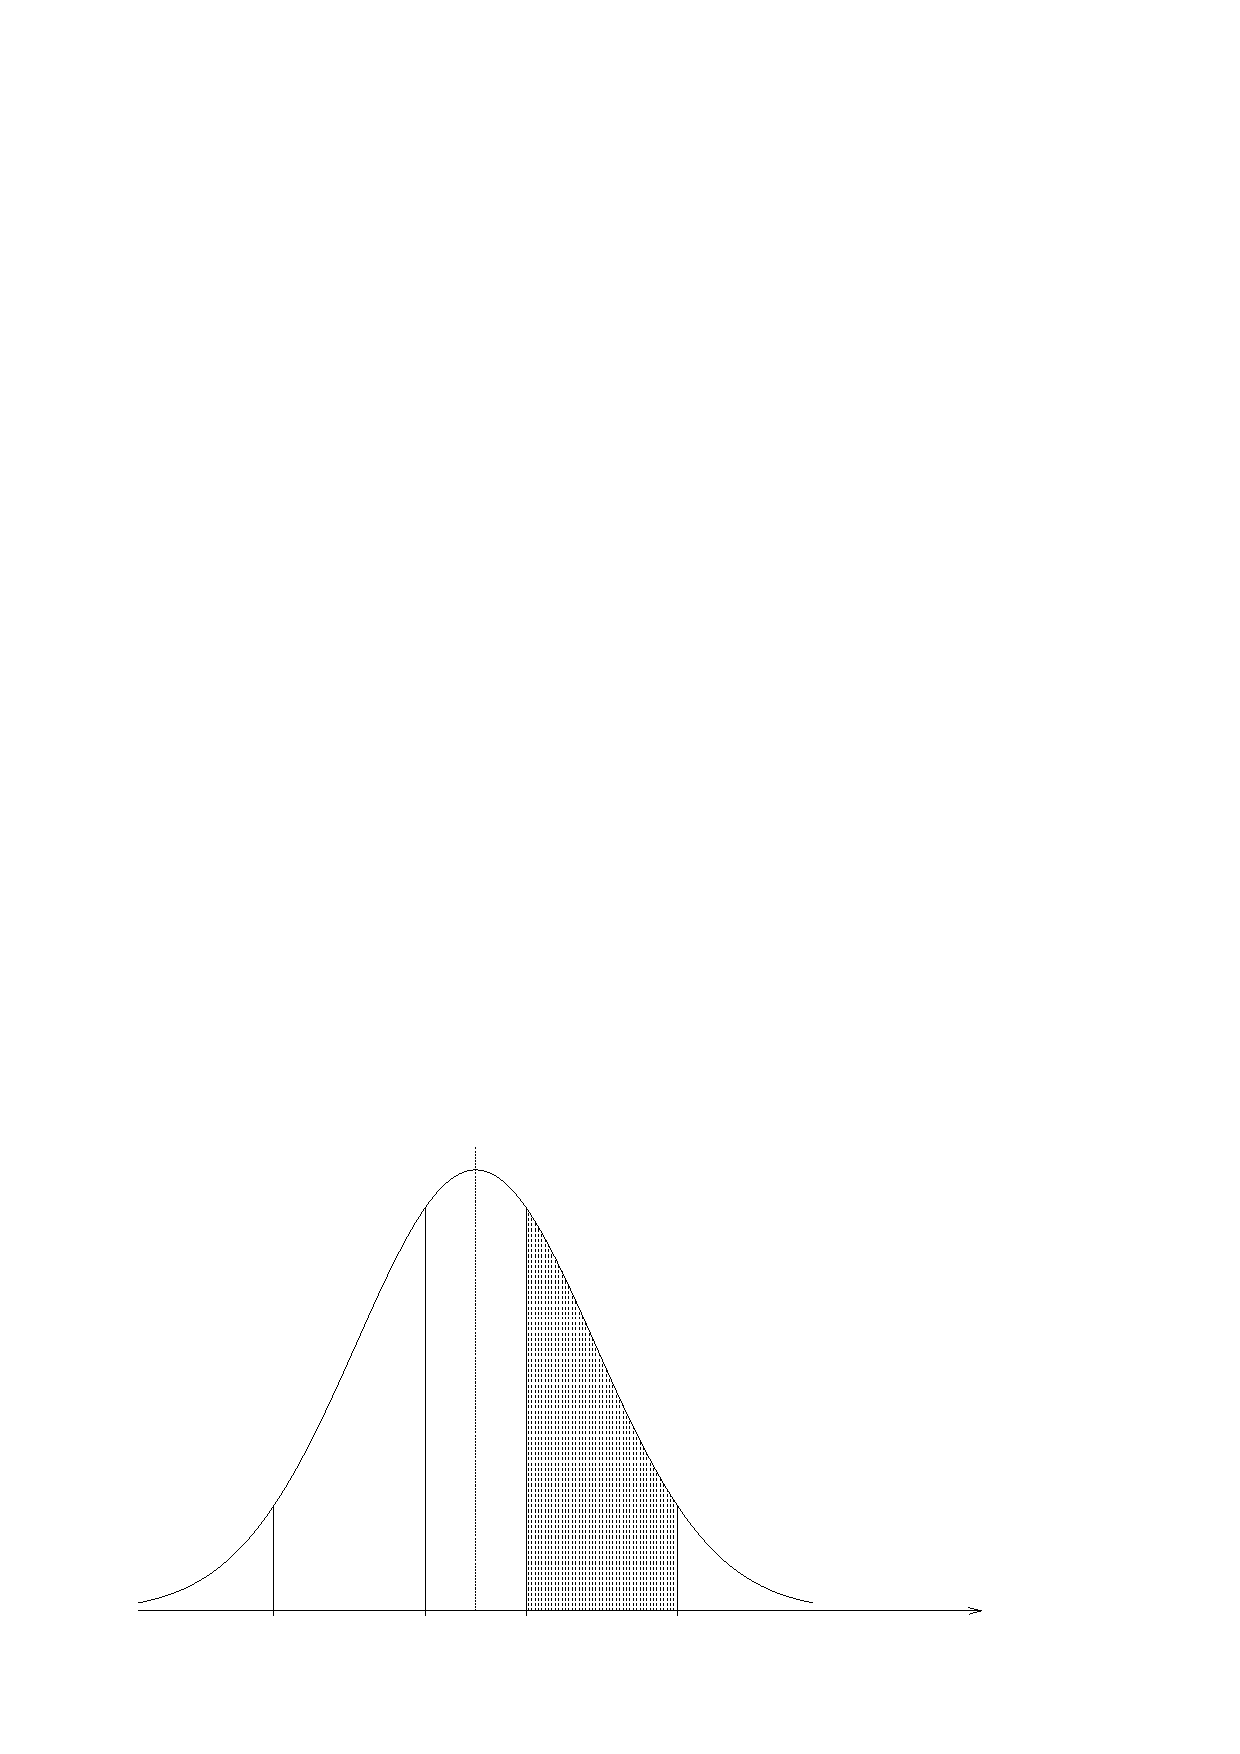
\includegraphics[width={360.00bp},height={252.00bp}]{fig-ordinal-1}}%
    \gplfronttext
  \end{picture}%
\endgroup

\caption{\label{fig:ordinal}Measurement equation for discrete indicators}
\end{figure}

The model specification for \PDBIOGEME\ is reported in Section
\ref{sec:02oneLatentOrdered}. Equation~\req{eq:likelihoodOrderedProbit}
is coded using the following statements:
\begin{lstlisting}
Envir01_tau_1 = (tau_1-MODEL_Envir01) / SIGMA_STAR_Envir01
Envir01_tau_2 = (tau_2-MODEL_Envir01) / SIGMA_STAR_Envir01
Envir01_tau_3 = (tau_3-MODEL_Envir01) / SIGMA_STAR_Envir01
Envir01_tau_4 = (tau_4-MODEL_Envir01) / SIGMA_STAR_Envir01
IndEnvir01 = {
    1: bioNormalCdf(Envir01_tau_1),
    2: bioNormalCdf(Envir01_tau_2)-bioNormalCdf(Envir01_tau_1),
    3: bioNormalCdf(Envir01_tau_3)-bioNormalCdf(Envir01_tau_2),
    4: bioNormalCdf(Envir01_tau_4)-bioNormalCdf(Envir01_tau_3),
    5: 1-bioNormalCdf(Envir01_tau_4),
    6: 1.0,
    -1: 1.0,
    -2: 1.0
}

P_Envir01 = Elem(IndEnvir01, Envir01)
\end{lstlisting}
Note that the indicators in the data file can take the values -2, -1, 1, 2,
3, 4, 5, and 6. However, the values 6, -1 and 2 are ignored, and
associated with a probability of 1, so that they have no influence on
the total likelihood function.

\begin{table}[htb]
\caption{\label{tab:ordered_output}Output of the Python script for
  ordered probit regression}
  \begin{lstlisting}
Estimated betas: 34
final log likelihood: -17794.883
Output file: 02oneLatentOrdered.html
LaTeX file: 02oneLatentOrdered.tex
  \end{lstlisting}
\end{table}
\begin{sidewaystable}[htb]
\caption{\label{tab:ordered}Estimation results for the ordered probit
  regression (first part)}
  \begin{tabular}{l}
\begin{tabular}{lr@{.}lr@{.}lr@{.}lr@{.}lr@{.}lr@{.}lr@{.}l}
                      &   \multicolumn{2}{l}{}    & \multicolumn{2}{l}{} & \multicolumn{2}{l}{}  &     \multicolumn{2}{l}{} &   \multicolumn{2}{l}{Robust}    & \multicolumn{2}{l}{Robust}  &     \multicolumn{2}{l}{Robust}   \\
Parameter      & \multicolumn{2}{l}{Estimate}  &
\multicolumn{2}{l}{std. err.}  &  \multicolumn{2}{l}{$t$-stat}  &   \multicolumn{2}{l}{$p$-value}  &
\multicolumn{2}{l}{std. err.}  &  \multicolumn{2}{l}{$t$-stat}  &   \multicolumn{2}{l}{$p$-value}   \\
\hline

B\_Envir02\_F1               &  -0&431 &   0&0558 &   -7&73 & 1&09e-14 &        0&0522 &        -8&25 &      2&22e-16 \\
B\_Envir03\_F1               &   0&566 &   0&0589 &     9&6 &      0&0 &         0&053 &         10&7 &           0&0 \\
B\_Mobil11\_F1               &   0&483 &   0&0583 &     8&3 &      0&0 &        0&0532 &         9&09 &           0&0 \\
B\_Mobil14\_F1               &   0&581 &   0&0584 &    9&95 &      0&0 &        0&0512 &         11&3 &           0&0 \\
B\_Mobil16\_F1               &   0&463 &   0&0559 &    8&28 & 2&22e-16 &        0&0542 &         8&54 &           0&0 \\
B\_Mobil17\_F1               &   0&368 &    0&055 &    6&69 & 2&25e-11 &        0&0518 &          7&1 &      1&27e-12 \\
INTER\_Envir02              &   0&349 &     0&03 &    11&6 &      0&0 &        0&0261 &         13&4 &           0&0 \\
INTER\_Envir03              &  -0&309 &   0&0311 &   -9&93 &      0&0 &         0&027 &        -11&4 &           0&0 \\
INTER\_Mobil11              &   0&338 &    0&031 &    10&9 &      0&0 &         0&029 &         11&7 &           0&0 \\
INTER\_Mobil14              &   -0&13 &     0&03 &   -4&34 & 1&44e-05 &         0&025 &        -5&21 &      1&94e-07 \\
INTER\_Mobil16              &   0&128 &   0&0288 &    4&45 & 8&42e-06 &        0&0276 &         4&65 &       3&3e-06 \\
INTER\_Mobil17              &   0&146 &   0&0281 &    5&18 & 2&16e-07 &         0&026 &         5&61 &      2&05e-08 \\
SIGMA\_STAR\_Envir02         &   0&767 &   0&0243 &    31&6 &      0&0 &        0&0222 &         34&6 &           0&0 \\
SIGMA\_STAR\_Envir03         &   0&718 &   0&0228 &    31&5 &      0&0 &        0&0206 &         34&9 &           0&0 \\
SIGMA\_STAR\_Mobil11         &   0&783 &   0&0254 &    30&8 &      0&0 &         0&024 &         32&6 &           0&0 \\
SIGMA\_STAR\_Mobil14         &   0&688 &   0&0217 &    31&7 &      0&0 &        0&0209 &         33&0 &           0&0 \\
SIGMA\_STAR\_Mobil16         &   0&754 &    0&024 &    31&5 &      0&0 &        0&0226 &         33&4 &           0&0 \\
SIGMA\_STAR\_Mobil17         &    0&76 &   0&0246 &    30&9 &      0&0 &        0&0235 &         32&3 &           0&0 \\
\hline
\end{tabular}
  \end{tabular}
\end{sidewaystable}

\begin{sidewaystable}[htb]
\caption{\label{tab:ordered2}Estimation results for the ordered probit
  regression (second part)}
  \begin{tabular}{l}
\begin{tabular}{lr@{.}lr@{.}lr@{.}lr@{.}lr@{.}lr@{.}lr@{.}l}
                      &   \multicolumn{2}{l}{}    & \multicolumn{2}{l}{} & \multicolumn{2}{l}{}  &     \multicolumn{2}{l}{} &   \multicolumn{2}{l}{Robust}    & \multicolumn{2}{l}{Robust}  &     \multicolumn{2}{l}{Robust}   \\
Parameter      & \multicolumn{2}{l}{Estimate}  &
\multicolumn{2}{l}{std. err.}  &  \multicolumn{2}{l}{$t$-stat}  &   \multicolumn{2}{l}{$p$-value}  &
\multicolumn{2}{l}{std. err.}  &  \multicolumn{2}{l}{$t$-stat}  &   \multicolumn{2}{l}{$p$-value}   \\
\hline
coef\_ContIncome\_0\_4000     &  0&0897 &   0&0375 &    2&39 &   0&0168 &        0&0528 &          1&7 &        0&0896 \\
coef\_ContIncome\_10000\_more &  0&0843 &   0&0207 &    4&07 &  4&6e-05 &        0&0303 &         2&78 &       0&00538 \\
coef\_ContIncome\_4000\_6000  &  -0&221 &   0&0642 &   -3&44 & 0&000583 &        0&0918 &        -2&41 &        0&0161 \\
coef\_ContIncome\_6000\_8000  &   0&259 &   0&0748 &    3&47 & 0&000525 &         0&109 &         2&37 &        0&0179 \\
coef\_ContIncome\_8000\_10000 &  -0&523 &   0&0883 &   -5&92 & 3&13e-09 &         0&128 &         -4&1 &      4&14e-05 \\
coef\_age\_65\_more           &  0&0718 &   0&0408 &    1&76 &   0&0787 &        0&0614 &         1&17 &         0&242 \\
coef\_haveChildren          & -0&0377 &   0&0302 &   -1&25 &    0&212 &        0&0459 &       -0&821 &         0&412 \\
coef\_haveGA                &  -0&578 &   0&0554 &   -10&4 &      0&0 &         0&075 &         -7&7 &      1&31e-14 \\
coef\_highEducation         &  -0&247 &   0&0353 &   -6&99 & 2&73e-12 &        0&0521 &        -4&73 &      2&22e-06 \\
coef\_individualHouse       & -0&0886 &   0&0312 &   -2&84 &  0&00453 &        0&0456 &        -1&94 &        0&0518 \\
coef\_intercept             &     0&4 &    0&109 &    3&66 & 0&000251 &         0&153 &         2&62 &       0&00884 \\
coef\_male                  &  0&0663 &   0&0281 &    2&36 &   0&0182 &        0&0433 &         1&53 &         0&125 \\
coef\_moreThanOneBike       &  -0&277 &   0&0381 &   -7&28 &  3&4e-13 &        0&0538 &        -5&15 &      2&56e-07 \\
coef\_moreThanOneCar        &   0&533 &   0&0427 &    12&5 &      0&0 &        0&0515 &         10&3 &           0&0 \\
delta\_1                    &   0&252 &  0&00716 &    35&2 &      0&0 &       0&00726 &         34&7 &           0&0 \\
delta\_2                    &   0&759 &   0&0187 &    40&6 &      0&0 &        0&0193 &         39&3 &           0&0 \\
\hline
\end{tabular}
\\
\begin{tabular}{rcl}
\multicolumn{3}{l}{\bf Summary statistics}\\
\multicolumn{3}{l}{ Number of observations = $1906$} \\
\multicolumn{3}{l}{ Number of excluded observations = $359$} \\
\multicolumn{3}{l}{ Number of estimated  parameters = $34$} \\
 $\mathcal{L}(\hat{\beta})$ &=& $-17794.88 $  \\

\end{tabular}
  \end{tabular}

\end{sidewaystable}


\clearpage

\section{Choice model}

Latent variables can be included in choice models. Consider a model
with three alternatives ``public transportation'' (PT), ``car'' (CAR)
and ``slow modes'' (SM). The utility functions are of the following form:
\begin{equation}
\label{eq:utility}
\begin{array}{rclclclcl}
U_{\text{PT}} &=& V_{\text{PT}} &+& \varepsilon_{\text{PT}} &=& \beta^t_\text{PT} \text{Time}_\text{PT} &+& \cdots + \varepsilon_{\text{PT}}\\
U_{\text{CAR}} &=&V_{\text{CAR}}&+& \varepsilon_{\text{CAR}} &=& \beta^t_\text{CAR} \text{Time}_\text{CAR} &+& \cdots
+ \varepsilon_{\text{CAR}}\\
U_{\text{SM}} &=&V_{\text{SM}} &+& \varepsilon_{\text{SM}}\\
\end{array}
\end{equation}
The full specification can be found in the specification
file in Section~\ref{sec:03choiceOnly}. 
 The
latent variable that we have considered in the previous sections captures the ``car loving'' attitude of the
individuals. In order to include it in the choice model, we specify that the coefficients
of travel time for the public transportation alternative, and for the
car alternative, vary with the latent variable. We have
\begin{equation}
\label{eq:beta_pt}
\beta^t_\text{PT} = \widehat{\beta}^t_\text{PT}
\exp(\beta^\text{CL}_\text{PT} x^*),
\end{equation}
and
\begin{equation}
\label{eq:beta_car}
\beta^t_\text{CAR} = \widehat{\beta}^t_\text{CAR}
\exp(\beta^\text{CL}_\text{CAR} x^*),
\end{equation}
where $x^*$ is defined by \req{eq:x_s}, so that
\begin{equation}
\beta^t_\text{PT} = \widehat{\beta}^t_\text{PT}
\exp(\beta^\text{CL}_\text{PT} (\bar{x}^s + \sigma_s \varepsilon^s)),
\end{equation}
and
\begin{equation}
\beta^t_\text{CAR} = \widehat{\beta}^t_\text{CAR}
\exp(\beta^\text{CL}_\text{CAR}(\bar{x}^s + \sigma_s \varepsilon^s)).
\end{equation}

Technically, such a choice model can be estimated using the choice observations
only, without the indicators. Assuming that $\varepsilon_{\text{PT}}$,
$\varepsilon_{\text{CAR}}$ and $\varepsilon_{\text{SM}}$ are
i.i.d. extreme value distributed, we have
\begin{equation}
\prob(\text{PT}|\varepsilon^s) = \frac{\exp(V_\text{PT})}{\exp(V_\text{PT})+\exp(V_\text{CAR})+\exp(V_\text{SM})} 
\end{equation}
and
\begin{equation}
  \label{eq:mixture_logit}
\prob(\text{PT}) =
\int_{\varepsilon=-\infty}^{\infty}\prob(\text{PT}|\varepsilon)\phi(\varepsilon) d\varepsilon,
\end{equation}
where $\phi(\cdot)$ is the probability density function of
the univariate standardized normal
distribution.
The choice model is a mixture of logit models.
The conditional probability $\prob(\text{PT}|\varepsilon)$ is
calculated using the statement
\begin{lstlisting}
condprob = models.logit(V,av,Choice)
\end{lstlisting}
and the integral in \req{eq:mixture_logit} by the statements
\begin{lstlisting}
omega = RandomVariable('omega')
density = dist.normalpdf(omega) 
prob = Integrate(condprob * density,'omega')
\end{lstlisting}

Note that it was not possible to estimate $\sigma_s$, which has then been
normalized to 1.

The output of the Python script is reported in
Table~\ref{tab:choiceOnly_output}.

The estimation results
are reported in Table~\ref{tab:choiceOnly}, where 
\begin{itemize}
\item \lstinline$BETA_TIME_PT_CL$ refers to $\beta^\protect\text{CL}_\protect\text{PT}$ in \req{eq:beta_pt},
\item \lstinline$BETA_TIME_PT_REF$ refers to $\widehat{\beta}^t_\protect\text{PT}$ in \req{eq:beta_pt},
\item \lstinline$BETA_TIME_CAR_CL$ refers to
  $\beta^\protect\text{CL}_\protect\text{CAR}$ in \req{eq:beta_car}, and
\item \lstinline$BETA_TIME_CAR_REF$ refers to $\widehat{\beta}^t_\protect\text{CAR}$ in \req{eq:beta_car}.
\end{itemize}

\begin{table}[htb]
\caption{\label{tab:choiceOnly_output}Output of the Python script for
  the mixture of logit models}
  \begin{lstlisting}
Estimated betas: 23
Final log likelihood: -1077.826
Output file: 03choiceOnly.html
LaTeX file: 03choiceOnly.tex
  \end{lstlisting}
\end{table}


\begin{sidewaystable}[htb]
\caption{\protect\label{tab:choiceOnly}Estimation results for the mixture of logit
models}
  \begin{tabular}{l}
\begin{tabular}{lr@{.}lr@{.}lr@{.}lr@{.}lr@{.}lr@{.}lr@{.}l}
                      &   \multicolumn{2}{l}{}    & \multicolumn{2}{l}{} & \multicolumn{2}{l}{}  &     \multicolumn{2}{l}{} &   \multicolumn{2}{l}{Robust}    & \multicolumn{2}{l}{Robust}  &     \multicolumn{2}{l}{Robust}   \\
Parameter      & \multicolumn{2}{l}{Estimate}  &
\multicolumn{2}{l}{std. err.}  &  \multicolumn{2}{l}{$t$-stat}  &   \multicolumn{2}{l}{$p$-value}  &
\multicolumn{2}{l}{std. err.}  &  \multicolumn{2}{l}{$t$-stat}  &   \multicolumn{2}{l}{$p$-value}   \\

\hline
ASC\_CAR                    &    0&41 &    0&156 &    2&64 &  0&00838 &         0&169 &         2&44 &        0&0149 \\
ASC\_SM                     &    1&01 &    0&261 &    3&88 & 0&000104 &         0&294 &         3&45 &      0&000554 \\
BETA\_COST\_HWH              &   -1&74 &    0&293 &   -5&92 & 3&25e-09 &         0&452 &        -3&84 &      0&000122 \\
BETA\_COST\_OTHER            &   -1&48 &    0&223 &   -6&62 & 3&67e-11 &         0&311 &        -4&74 &      2&14e-06 \\
BETA\_DIST                  &   -4&87 &    0&546 &   -8&92 &      0&0 &         0&635 &        -7&67 &      1&69e-14 \\
BETA\_TIME\_CAR\_CL           &  -0&508 &     0&04 &   -12&7 &      0&0 &        0&0492 &        -10&3 &           0&0 \\
BETA\_TIME\_CAR\_REF          &   -25&7 &     4&99 &   -5&15 & 2&66e-07 &          5&61 &        -4&58 &      4&76e-06 \\
BETA\_TIME\_PT\_CL            &   -1&78 &    0&146 &   -12&1 &      0&0 &         0&211 &        -8&43 &           0&0 \\
BETA\_TIME\_PT\_REF           &   -4&69 &     2&54 &   -1&85 &    0&065 &          2&49 &        -1&89 &        0&0591 \\
BETA\_WAITING\_TIME          & -0&0528 &    0&012 &   -4&38 & 1&17e-05 &        0&0188 &        -2&81 &       0&00493 \\
coef\_ContIncome\_0\_4000     & -0&0903 &   0&0917 &  -0&984 &    0&325 &        0&0821 &         -1&1 &         0&271 \\
coef\_ContIncome\_10000\_more &  -0&104 &   0&0449 &   -2&31 &   0&0209 &        0&0397 &        -2&61 &        0&0091 \\
coef\_ContIncome\_4000\_6000  &  0&0851 &    0&144 &   0&592 &    0&554 &        0&0997 &        0&853 &         0&393 \\
coef\_ContIncome\_6000\_8000  &   -0&23 &    0&166 &   -1&39 &    0&165 &         0&128 &         -1&8 &         0&072 \\
coef\_ContIncome\_8000\_10000 &   0&357 &    0&193 &    1&85 &   0&0644 &         0&155 &         2&31 &        0&0211 \\
coef\_age\_65\_more           &    0&18 &    0&116 &    1&56 &    0&119 &         0&111 &         1&62 &         0&105 \\
coef\_haveChildren          &  0&0477 &    0&065 &   0&734 &    0&463 &        0&0515 &        0&927 &         0&354 \\
coef\_haveGA                &    1&49 &    0&136 &    11&0 &      0&0 &         0&114 &         13&1 &           0&0 \\
coef\_highEducation         &  -0&494 &   0&0724 &   -6&82 & 9&08e-12 &         0&063 &        -7&83 &      4&88e-15 \\
coef\_individualHouse       &   0&021 &    0&084 &    0&25 &    0&803 &        0&0925 &        0&227 &          0&82 \\
coef\_male                  &   -0&12 &   0&0714 &   -1&67 &    0&094 &        0&0744 &        -1&61 &         0&108 \\
coef\_moreThanOneBike       &   0&118 &    0&096 &    1&23 &     0&22 &        0&0766 &         1&53 &         0&125 \\
coef\_moreThanOneCar        &  -0&603 &     0&06 &   -10&0 &      0&0 &        0&0367 &        -16&4 &           0&0 \\

\hline
\end{tabular}
\\
\begin{tabular}{rcl}
\multicolumn{3}{l}{\bf Summary statistics}\\
\multicolumn{3}{l}{ Number of observations = $1906$} \\
\multicolumn{3}{l}{ Number of excluded observations = $359$} \\
\multicolumn{3}{l}{ Number of estimated  parameters = $23$} \\
 $\mathcal{L}(\beta_0)$ &=&  $-2093.955$ \\
 $\mathcal{L}(\hat{\beta})$ &=& $-1077.826 $  \\
 $-2[\mathcal{L}(\beta_0) -\mathcal{L}(\hat{\beta})]$ &=& $2032.257$ \\
    $\rho^2$ &=&   $0.485$ \\
    $\bar{\rho}^2$ &=&    $0.474$ \\
\end{tabular}
  \end{tabular}
\end{sidewaystable}


\clearpage 

\section{Sequential estimation}

In order to exploit both the choice data and the psychometric
indicator, we now combine the latent variable model with the choice
model. The easiest way to estimate a joint model is using sequential
estimation. However, such an estimator is not efficient, and a full
information estimation is preferable. It is described in Section~\ref{sec:fi}.

For the sequential estimation, we use \req{eq:x_s} in \req{eq:beta_pt} and
\req{eq:beta_car}, where the values of the coefficients $\beta^s$ are
the result of the estimation  presented in
Table~\ref{tab:ordered}. We have again a mixture of logit models, but
with fewer parameters, as the parameters of the structural equation
are not re-estimated. The specification file is presented in
Section~\ref{sec:04latentChoiceSeq}. The estimated parameters of the
choice model are presented in Table~\ref{tab:sequential}.

It is important to realize that the estimation results in
Tables~\ref{tab:choiceOnly} and \ref{tab:sequential} cannot be
compared, as their specifications are not using the same variables. 

\begin{table}[htb]
\caption{\label{tab:sequential_output}Output of the Python script for the sequential estimation}
  \begin{lstlisting}
Estimated betas: 11
Final log likelihood: -1092.592
Output file: 04latentChoiceSeq.html
LaTeX file: 04latentChoiceSeq.tex
  \end{lstlisting}
\end{table}



 \begin{sidewaystable}[htb]
\caption{\label{tab:sequential}Estimation results for the sequential estimation}
  \begin{tabular}{l}
\begin{tabular}{lr@{.}lr@{.}lr@{.}lr@{.}lr@{.}lr@{.}lr@{.}l}
                      &   \multicolumn{2}{l}{}    & \multicolumn{2}{l}{} & \multicolumn{2}{l}{}  &     \multicolumn{2}{l}{} &   \multicolumn{2}{l}{Robust}    & \multicolumn{2}{l}{Robust}  &     \multicolumn{2}{l}{Robust}   \\
Parameter      & \multicolumn{2}{l}{Estimate}  &
\multicolumn{2}{l}{std. err.}  &  \multicolumn{2}{l}{$t$-stat}  &   \multicolumn{2}{l}{$p$-value}  &
\multicolumn{2}{l}{std. err.}  &  \multicolumn{2}{l}{$t$-stat}  &   \multicolumn{2}{l}{$p$-value}   \\
\hline
ASC\_CAR           &   0&773 &    0&127 &    6&11 & 1&02e-09 &         0&127 &         6&07 &      1&31e-09 \\
ASC\_SM            &    1&88 &    0&242 &    7&78 & 7&55e-15 &         0&241 &         7&82 &      5&33e-15 \\
BETA\_COST\_HWH     &   -1&78 &    0&305 &   -5&84 & 5&15e-09 &         0&492 &        -3&62 &      0&000293 \\
BETA\_COST\_OTHER   &  -0&818 &    0&172 &   -4&76 & 1&98e-06 &         0&268 &        -3&05 &        0&0023 \\
BETA\_DIST         &    -5&8 &    0&704 &   -8&24 & 2&22e-16 &         0&704 &        -8&24 &      2&22e-16 \\
BETA\_TIME\_CAR\_CL  &   -1&68 &   0&0737 &   -22&8 &      0&0 &        0&0626 &        -26&9 &           0&0 \\
BETA\_TIME\_CAR\_REF &   -17&7 &     2&31 &   -7&65 &  2e-14&0 &          2&53 &         -7&0 &      2&64e-12 \\
BETA\_TIME\_PT\_CL   &   -1&24 &   0&0643 &   -19&3 &      0&0 &         0&047 &        -26&4 &           0&0 \\
BETA\_TIME\_PT\_REF  &   -6&27 &    0&935 &   -6&71 & 1&95e-11 &          0&94 &        -6&67 &      2&48e-11 \\
BETA\_WAITING\_TIME & -0&0295 &   0&0104 &   -2&84 &  0&00451 &        0&0151 &        -1&95 &        0&0511 \\
sigma\_s           &   0&862 &   0&0366 &    23&5 &      0&0 &        0&0247 &         34&9 &           0&0 \\

\hline
\end{tabular}
\\
\begin{tabular}{rcl}
\multicolumn{3}{l}{\bf Summary statistics}\\
\multicolumn{3}{l}{ Number of observations = $1906$} \\
\multicolumn{3}{l}{ Number of excluded observations = $359$} \\
\multicolumn{3}{l}{ Number of estimated  parameters = $11$} \\
 $\mathcal{L}(\beta_0)$ &=&  $-2093.955$ \\
 $\mathcal{L}(\hat{\beta})$ &=& $-1092.592 $  \\
 $-2[\mathcal{L}(\beta_0) -\mathcal{L}(\hat{\beta})]$ &=& $2002.726$ \\
    $\rho^2$ &=&   $0.478$ \\
    $\bar{\rho}^2$ &=&    $0.473$ \\
\end{tabular}
  \end{tabular}
 \end{sidewaystable}

\clearpage

\section{Full information estimation}
\label{sec:fi}
The proper way of estimating the model is to jointly estimate the
parameters of the structural equation and the
parameters of the choice model, using both the indicators and the
choice data. 

As the latent variable, and therefore $\varepsilon^s$, is involved in
both the measurement equations for the indicators, and the measurement
equations of the choice model, the joint likelihood must be first
calculated conditional on $\varepsilon^s$:
\begin{equation}
\label{eq:fiLike1}
\mathcal{L}_n(\varepsilon_s) = P_n(i_n|\varepsilon_s) \prod_{i} \prob(I_i = j_{in}|\varepsilon_s),  
\end{equation}
where $i_n$ is the observed choice of individual $n$, and $j_{in}$ is
the response of individual $n$ to the psychometric question  $i$. The
contribution to the likelihood of this individual is then
\begin{equation}
\label{eq:fiLike2}
\begin{array}{rcl}
\mathcal{L}_n &=& \displaystyle\int_{\varepsilon=-\infty}^{+\infty}
\mathcal{L}_n(\varepsilon) \phi(\varepsilon)d\varepsilon \\ && \\
&=& \displaystyle\int_{\varepsilon=-\infty}^{+\infty}P_n(i_n|\varepsilon_s) \prod_{i} \prob(I_i = j_{in}|\varepsilon_s) \phi(\varepsilon)d\varepsilon.
\end{array}
\end{equation}
 
The specification file is provided in
Section~\ref{sec:05latentChoiceFull}, and the estimation results in
Tables~\ref{tab:fi} and \ref{tab:fi-2}.

Note that such models are particularly difficult to estimate. In this
case, Biogeme was able to perform the estimation, but there is a
numerical issue with the Rao-Cramer bound. The standard error of the
parameter \lstinline+BETA_TIME_PT_CL+ is reported as \lstinline+nan+,
which stands for ``not a number''. It has been generated by Biogeme's attempt to take the
square root of a negative number. Another sign of this numerical issue
is the negative eigenvalue (-14.6744) that shows that the estimate of
the variance-covariance matrix is not positive definite in this
case. The robust version of the statistics must be used in this case. 

\begin{table}[htb]
\caption{\label{tab:fi_output}Output of the Python script for the full
information estimation}
  \begin{lstlisting}
Estimated betas: 45
Final log likelihood: -18406.146
Output file: 05latentChoiceFull.html
LaTeX file: 05latentChoiceFull.tex
  \end{lstlisting}
\end{table}



 \begin{sidewaystable}[htb]
\caption{\label{tab:fi}Estimation results for the full information
  estimation (first part)}
\begin{tabular}{lr@{.}lr@{.}lr@{.}lr@{.}lr@{.}lr@{.}lr@{.}l}
                      &   \multicolumn{2}{l}{}    & \multicolumn{2}{l}{} & \multicolumn{2}{l}{}  &     \multicolumn{2}{l}{} &   \multicolumn{2}{l}{Robust}    & \multicolumn{2}{l}{Robust}  &     \multicolumn{2}{l}{Robust}   \\
Parameter      & \multicolumn{2}{l}{Estimate}  &
\multicolumn{2}{l}{std. err.}  &  \multicolumn{2}{l}{$t$-stat}  &   \multicolumn{2}{l}{$p$-value}  &
\multicolumn{2}{l}{std. err.}  &  \multicolumn{2}{l}{$t$-stat}  &   \multicolumn{2}{l}{$p$-value}   \\

\hline

ASC\_CAR                    &    1&08 &   0&0919 &    11&8 &      0&0 &        0&0974 &         11&1 &           0&0 \\
ASC\_SM                     &   0&525 &    0&173 &    3&04 &  0&00236 &         0&316 &         1&66 &        0&0968 \\
BETA\_COST\_HWH              &   -1&38 &    0&221 &   -6&22 & 4&82e-10 &         0&323 &        -4&26 &      2&06e-05 \\
BETA\_COST\_OTHER            &  -0&654 &    0&114 &   -5&76 & 8&59e-09 &         0&162 &        -4&03 &      5&46e-05 \\
BETA\_DIST                  &    -1&1 &   0&0997 &   -11&1 &      0&0 &         0&252 &        -4&38 &      1&18e-05 \\
BETA\_TIME\_CAR\_CL           &   -1&06 &    0&145 &   -7&31 &  2&7e-13 &         0&202 &        -5&23 &      1&73e-07 \\
BETA\_TIME\_CAR\_REF          &   -4&84 &    0&643 &   -7&54 & 4&82e-14 &         0&877 &        -5&52 &      3&32e-08 \\
BETA\_TIME\_PT\_CL            &   -1&25 &    \multicolumn{2}{c}{nan} &     0&0 &      1&0 &         0&299 &        -4&16 &      3&16e-05 \\
BETA\_TIME\_PT\_REF           & -0&0001 &  0&00237 & -0&0422 &    0&966 &      2&07e-05 &        -4&82 &      1&42e-06 \\
BETA\_WAITING\_TIME          & -0&0442 &  0&00715 &   -6&19 & 5&98e-10 &       0&00943 &        -4&69 &      2&75e-06 \\
B\_Envir02\_F1               &  -0&456 &   0&0314 &   -14&5 &      0&0 &        0&0307 &        -14&8 &           0&0 \\
B\_Envir03\_F1               &   0&483 &   0&0317 &    15&2 &      0&0 &        0&0316 &         15&3 &           0&0 \\
B\_Mobil11\_F1               &    0&57 &   0&0371 &    15&3 &      0&0 &        0&0422 &         13&5 &           0&0 \\
B\_Mobil14\_F1               &   0&575 &   0&0332 &    17&3 &      0&0 &        0&0349 &         16&5 &           0&0 \\
B\_Mobil16\_F1               &   0&526 &    0&035 &    15&0 &      0&0 &        0&0426 &         12&3 &           0&0 \\
B\_Mobil17\_F1               &   0&519 &   0&0355 &    14&6 &      0&0 &        0&0425 &         12&2 &           0&0 \\
INTER\_Envir02              &   0&459 &   0&0319 &    14&4 &      0&0 &        0&0309 &         14&8 &           0&0 \\
INTER\_Envir03              &  -0&367 &   0&0299 &   -12&3 &      0&0 &         0&029 &        -12&7 &           0&0 \\
INTER\_Mobil11              &    0&42 &   0&0349 &    12&0 &      0&0 &        0&0376 &         11&2 &           0&0 \\
INTER\_Mobil14              &  -0&173 &   0&0282 &   -6&13 & 9&01e-10 &        0&0278 &        -6&22 &      5&09e-10 \\
INTER\_Mobil16              &   0&147 &   0&0304 &    4&83 & 1&33e-06 &        0&0338 &         4&35 &      1&35e-05 \\
INTER\_Mobil17              &   0&138 &   0&0309 &    4&47 &  7&9e-06 &        0&0333 &         4&14 &      3&43e-05 \\
SIGMA\_STAR\_Envir02         &    0&92 &    0&034 &    27&0 &      0&0 &        0&0346 &         26&6 &           0&0 \\
SIGMA\_STAR\_Envir03         &   0&858 &   0&0329 &    26&1 &      0&0 &        0&0354 &         24&3 &           0&0 \\
SIGMA\_STAR\_Mobil11         &   0&897 &   0&0366 &    24&5 &      0&0 &        0&0413 &         21&7 &           0&0 \\
SIGMA\_STAR\_Mobil14         &   0&761 &   0&0306 &    24&8 &      0&0 &        0&0334 &         22&8 &           0&0 \\
SIGMA\_STAR\_Mobil16         &   0&873 &   0&0352 &    24&8 &      0&0 &          0&04 &         21&8 &           0&0 \\
SIGMA\_STAR\_Mobil17         &   0&875 &   0&0353 &    24&8 &      0&0 &        0&0396 &         22&1 &           0&0 \\
\hline
\end{tabular}
 \end{sidewaystable}

 \begin{sidewaystable}[htb]
\caption{\label{tab:fi-2}Estimation results for the full information
  estimation (second part)}

  \begin{tabular}{l}
\begin{tabular}{lr@{.}lr@{.}lr@{.}lr@{.}lr@{.}lr@{.}lr@{.}l}
                      &   \multicolumn{2}{l}{}    & \multicolumn{2}{l}{} & \multicolumn{2}{l}{}  &     \multicolumn{2}{l}{} &   \multicolumn{2}{l}{Robust}    & \multicolumn{2}{l}{Robust}  &     \multicolumn{2}{l}{Robust}   \\
Parameter      & \multicolumn{2}{l}{Estimate}  &
\multicolumn{2}{l}{std. err.}  &  \multicolumn{2}{l}{$t$-stat}  &   \multicolumn{2}{l}{$p$-value}  &
\multicolumn{2}{l}{std. err.}  &  \multicolumn{2}{l}{$t$-stat}  &   \multicolumn{2}{l}{$p$-value}   \\
\hline
coef\_ContIncome\_0\_4000     &   0&151 &   0&0616 &    2&45 &   0&0141 &        0&0624 &         2&43 &        0&0153 \\
coef\_ContIncome\_10000\_more &    0&12 &   0&0371 &    3&23 &  0&00123 &        0&0367 &         3&27 &       0&00108 \\
coef\_ContIncome\_4000\_6000  &   -0&29 &    0&113 &   -2&57 &   0&0103 &         0&116 &        -2&51 &        0&0122 \\
coef\_ContIncome\_6000\_8000  &    0&34 &    0&134 &    2&54 &   0&0109 &         0&138 &         2&46 &        0&0137 \\
coef\_ContIncome\_8000\_10000 &  -0&684 &    0&155 &   -4&42 &  9&7e-06 &         0&158 &        -4&34 &      1&46e-05 \\
coef\_age\_65\_more           &  0&0358 &   0&0743 &   0&482 &     0&63 &        0&0753 &        0&476 &         0&634 \\
coef\_haveChildren          & -0&0278 &   0&0557 &  -0&499 &    0&618 &        0&0567 &       -0&491 &         0&624 \\
coef\_haveGA                &   -0&75 &    0&093 &   -8&07 & 6&66e-16 &         0&101 &        -7&46 &      8&86e-14 \\
coef\_highEducation         &  -0&259 &   0&0604 &    -4&3 & 1&74e-05 &        0&0676 &        -3&84 &      0&000125 \\
coef\_individualHouse       &  -0&116 &   0&0567 &   -2&05 &   0&0406 &        0&0564 &        -2&06 &        0&0395 \\
coef\_intercept             &    0&35 &    0&174 &    2&01 &   0&0447 &         0&174 &         2&01 &        0&0447 \\
coef\_male                  &  0&0795 &   0&0512 &    1&55 &    0&121 &        0&0537 &         1&48 &         0&139 \\
coef\_moreThanOneBike       &  -0&362 &   0&0657 &   -5&51 & 3&56e-08 &        0&0694 &        -5&22 &      1&79e-07 \\
coef\_moreThanOneCar        &   0&715 &   0&0636 &    11&2 &      0&0 &        0&0672 &         10&6 &           0&0 \\
delta\_1                    &   0&328 &   0&0113 &    29&0 &      0&0 &        0&0128 &         25&7 &           0&0 \\
delta\_2                    &   0&991 &   0&0313 &    31&7 &      0&0 &        0&0361 &         27&5 &           0&0 \\
sigma\_s                    &   0&862 &    0&048 &    17&9 &      0&0 &        0&0557 &         15&5 &           0&0 \\

\hline
\end{tabular}
\\
\begin{tabular}{rcl}
\multicolumn{3}{l}{\bf Summary statistics}\\
\multicolumn{3}{l}{ Number of observations = $1906$} \\
\multicolumn{3}{l}{ Number of excluded observations = $359$} \\
\multicolumn{3}{l}{ Number of estimated  parameters = $45$} \\
 $\mathcal{L}(\hat{\beta})$ &=& $-18406.15 $  \\
\end{tabular}
  \end{tabular}
 \end{sidewaystable}

\clearpage

\section{Serial correlation}

The likelihood function \req{eq:fiLike1}--\req{eq:fiLike2} assumes
that the error terms involved in the models are independent, that is,
$\varepsilon^{m}_i$ in \req{eq:x_m}, and the errors terms of the utility
functions \req{eq:utility}. However, because all these models apply to
the same individual who made the choice and provided the indicators,
these error terms may actually be correlated as they potentially share
unobserved variables specific to this individual. This issue, called
serial correlation, can be handled by including an agent effect in the
model specification. This is an error component appearing in all the
models involved, distributed across the individuals.

The specification file is provided in
Section~\ref{sec:06serialCorrelation}, and the estimation results in
Tables~\ref{tab:fi-sc} and \ref{tab:fi-sc-2}. In our example, the
parameter of the agent effect appears not to be significant, with a
$p$-value of 0.82. Note also that the integral is approximated here
using Monte-Carlo simulation. 

\begin{table}[htb]
\caption{\label{tab:fi_sc_output}Output of the Python script for the
  full information estimation with agent effect}
  \begin{lstlisting}
Estimated betas: 46
Final log likelihood: -18559.078
Output file: 06serialCorrelation.html
LaTeX file: 06serialCorrelation.tex
  \end{lstlisting}
\end{table}




 \begin{sidewaystable}[htb]
\caption{\label{tab:fi-sc}Estimation results for the full information
  estimation with agent effect (first part)}
\begin{tabular}{lr@{.}lr@{.}lr@{.}lr@{.}lr@{.}lr@{.}lr@{.}l}
                      &   \multicolumn{2}{l}{}    & \multicolumn{2}{l}{} & \multicolumn{2}{l}{}  &     \multicolumn{2}{l}{} &   \multicolumn{2}{l}{Robust}    & \multicolumn{2}{l}{Robust}  &     \multicolumn{2}{l}{Robust}   \\
Parameter      & \multicolumn{2}{l}{Estimate}  &
\multicolumn{2}{l}{std. err.}  &  \multicolumn{2}{l}{$t$-stat}  &   \multicolumn{2}{l}{$p$-value}  &
\multicolumn{2}{l}{std. err.}  &  \multicolumn{2}{l}{$t$-stat}  &   \multicolumn{2}{l}{$p$-value}   \\
\hline
ASC\_CAR                    &   0&656 &    0&113 &    5&81 & 6&32e-09 &         0&127 &         5&17 &      2&32e-07 \\
ASC\_SM                     &   0&115 &    0&191 &   0&603 &    0&547 &         0&359 &        0&321 &         0&748 \\
BETA\_COST\_HWH              &   -1&33 &    0&204 &   -6&54 & 6&27e-11 &          0&46 &         -2&9 &       0&00374 \\
BETA\_COST\_OTHER            &  -0&521 &    0&127 &   -4&12 & 3&85e-05 &         0&285 &        -1&83 &        0&0672 \\
BETA\_DIST                  &   -1&42 &    0&128 &   -11&1 &      0&0 &          0&39 &        -3&64 &      0&000277 \\
BETA\_TIME\_CAR\_CL           &  -0&993 &    0&125 &   -7&94 &  2e-15&0 &         0&173 &        -5&74 &      9&23e-09 \\
BETA\_TIME\_CAR\_REF          &   -9&36 &     1&06 &   -8&84 &      0&0 &          2&07 &        -4&51 &      6&34e-06 \\
BETA\_TIME\_PT\_CL            &  -0&356 &    0&141 &   -2&53 &   0&0115 &         0&203 &        -1&75 &        0&0801 \\
BETA\_TIME\_PT\_REF           &   -3&03 &    0&528 &   -5&74 & 9&28e-09 &         0&903 &        -3&36 &      0&000773 \\
BETA\_WAITING\_TIME          &  -0&023 &  0&00816 &   -2&82 &   0&0048 &        0&0119 &        -1&94 &        0&0526 \\
B\_Envir02\_F1               &  -0&448 &   0&0345 &   -13&0 &      0&0 &        0&0331 &        -13&5 &           0&0 \\
B\_Envir03\_F1               &   0&499 &   0&0364 &    13&7 &      0&0 &        0&0598 &         8&35 &           0&0 \\
B\_Mobil11\_F1               &   0&601 &   0&0415 &    14&5 &      0&0 &        0&0519 &         11&6 &           0&0 \\
B\_Mobil14\_F1               &   0&601 &   0&0371 &    16&2 &      0&0 &         0&048 &         12&5 &           0&0 \\
B\_Mobil16\_F1               &   0&544 &   0&0387 &    14&1 &      0&0 &        0&0499 &         10&9 &           0&0 \\
B\_Mobil17\_F1               &   0&531 &   0&0389 &    13&7 &      0&0 &        0&0437 &         12&1 &           0&0 \\
INTER\_Envir02              &   0&425 &   0&0304 &    14&0 &      0&0 &        0&0295 &         14&4 &           0&0 \\
INTER\_Envir03              &  -0&349 &   0&0291 &   -12&0 &      0&0 &        0&0296 &        -11&8 &           0&0 \\
INTER\_Mobil11              &   0&375 &   0&0333 &    11&3 &      0&0 &        0&0401 &         9&34 &           0&0 \\
INTER\_Mobil14              &  -0&171 &   0&0282 &   -6&07 & 1&31e-09 &        0&0283 &        -6&05 &      1&46e-09 \\
INTER\_Mobil16              &   0&127 &   0&0296 &    4&29 & 1&76e-05 &        0&0348 &         3&66 &      0&000257 \\
INTER\_Mobil17              &   0&122 &   0&0299 &    4&09 & 4&28e-05 &         0&032 &         3&82 &      0&000132 \\
SIGMA\_STAR\_Envir02         &   0&875 &   0&0306 &    28&7 &      0&0 &        0&0344 &         25&5 &           0&0 \\
SIGMA\_STAR\_Envir03         &   0&811 &   0&0297 &    27&4 &      0&0 &        0&0436 &         18&6 &           0&0 \\
SIGMA\_STAR\_Mobil11         &   0&846 &   0&0321 &    26&3 &      0&0 &        0&0399 &         21&2 &           0&0 \\
SIGMA\_STAR\_Mobil14         &   0&724 &   0&0271 &    26&7 &      0&0 &        0&0363 &         19&9 &           0&0 \\
SIGMA\_STAR\_Mobil16         &   0&828 &   0&0309 &    26&8 &      0&0 &         0&038 &         21&8 &           0&0 \\
SIGMA\_STAR\_Mobil17         &   0&831 &    0&031 &    26&8 &      0&0 &        0&0357 &         23&3 &           0&0 \\
\hline
\end{tabular}
 \end{sidewaystable}

 \begin{sidewaystable}[htb]
\caption{\label{tab:fi-sc-2}Estimation results for the full information
  estimation with agent effect (second part)}
  \begin{tabular}{l}
\begin{tabular}{lr@{.}lr@{.}lr@{.}lr@{.}lr@{.}lr@{.}lr@{.}l}
                      &   \multicolumn{2}{l}{}    & \multicolumn{2}{l}{} & \multicolumn{2}{l}{}  &     \multicolumn{2}{l}{} &   \multicolumn{2}{l}{Robust}    & \multicolumn{2}{l}{Robust}  &     \multicolumn{2}{l}{Robust}   \\
Parameter      & \multicolumn{2}{l}{Estimate}  &
\multicolumn{2}{l}{std. err.}  &  \multicolumn{2}{l}{$t$-stat}  &   \multicolumn{2}{l}{$p$-value}  &
\multicolumn{2}{l}{std. err.}  &  \multicolumn{2}{l}{$t$-stat}  &   \multicolumn{2}{l}{$p$-value}   \\
\hline
coef\_ContIncome\_0\_4000     &   0&147 &    0&048 &    3&07 &  0&00217 &        0&0782 &         1&88 &        0&0597 \\
coef\_ContIncome\_10000\_more &   0&128 &   0&0297 &    4&32 & 1&57e-05 &        0&0515 &         2&49 &        0&0127 \\
coef\_ContIncome\_4000\_6000  &  -0&314 &   0&0923 &    -3&4 & 0&000669 &          0&22 &        -1&43 &         0&153 \\
coef\_ContIncome\_6000\_8000  &   0&396 &    0&106 &    3&73 & 0&000191 &           0&2 &         1&98 &         0&048 \\
coef\_ContIncome\_8000\_10000 &  -0&687 &    0&124 &   -5&55 & 2&87e-08 &         0&221 &        -3&11 &       0&00186 \\
coef\_age\_65\_more           &  0&0236 &   0&0601 &   0&393 &    0&694 &        0&0872 &        0&271 &         0&786 \\
coef\_haveChildren          & -0&0451 &   0&0495 &  -0&911 &    0&362 &         0&146 &        -0&31 &         0&757 \\
coef\_haveGA                &  -0&655 &   0&0727 &    -9&0 &      0&0 &        0&0971 &        -6&74 &      1&55e-11 \\
coef\_highEducation         &  -0&232 &   0&0483 &   -4&79 & 1&63e-06 &        0&0746 &         -3&1 &       0&00191 \\
coef\_individualHouse       & -0&0551 &   0&0467 &   -1&18 &    0&238 &        0&0908 &       -0&607 &         0&544 \\
coef\_intercept             &   0&265 &    0&134 &    1&97 &   0&0483 &         0&164 &         1&62 &         0&106 \\
coef\_male                  &  0&0652 &   0&0408 &     1&6 &     0&11 &        0&0589 &         1&11 &         0&268 \\
coef\_moreThanOneBike       &  -0&319 &   0&0533 &   -5&99 &  2&1e-09 &        0&0905 &        -3&53 &      0&000423 \\
coef\_moreThanOneCar        &   0&615 &   0&0534 &    11&5 &      0&0 &         0&102 &         6&05 &      1&45e-09 \\
delta\_1                    &   0&306 &  0&00989 &    30&9 &      0&0 &        0&0134 &         22&9 &           0&0 \\
delta\_2                    &    0&92 &   0&0269 &    34&2 &      0&0 &        0&0399 &         23&1 &           0&0 \\
ec\_sigma                   &   0&694 &   0&0612 &    11&3 &      0&0 &         0&264 &         2&63 &       0&00848 \\
sigma\_s                    &   0&272 &    0&146 &    1&87 &   0&0617 &         0&807 &        0&337 &         0&736 \\
\hline
\end{tabular}
\\
\begin{tabular}{rcl}
\multicolumn{3}{l}{\bf Summary statistics}\\
\multicolumn{3}{l}{ Number of observations = $1906$} \\
\multicolumn{3}{l}{ Number of excluded observations = $359$} \\
\multicolumn{3}{l}{ Number of estimated  parameters = $46$} \\
 $\mathcal{L}(\hat{\beta})$ &=& $-18559.08 $  \\
\end{tabular}
  \end{tabular}

 \end{sidewaystable}

\clearpage



\section{Discussions}

We conclude with some comments this short introduction to the estimation of choice models
with latent variables.
\begin{itemize}
\item The initial values of the $\sigma$ parameters involved in the
  model specification should be large enough, and in any case
  certainly not 0. Indeed, if they are too
  small, the likelihood of some observations may be so small that they
  are numerically 0. Therefore, calculating the log likelihood is
  impossible and the estimation will fail even before the first
  iteration. PandasBiogeme will raise an exception:
  \begin{lstlisting}
Traceback (most recent call last):
  File "07problem.py", line 270, in <module>
    results = biogeme.estimate()
  File "/usr/local/lib/python3.7/site-packages/biogeme-3.1.0-py3.7-macosx-10.13-x86_64.egg/biogeme/biogeme.py", line 349, in estimate
    self.calculateInitLikelihood()
  File "/usr/local/lib/python3.7/site-packages/biogeme-3.1.0-py3.7-macosx-10.13-x86_64.egg/biogeme/biogeme.py", line 226, in calculateInitLikelihood
    self.initLogLike = self.calculateLikelihood(self.betaInitValues)
  File "/usr/local/lib/python3.7/site-packages/biogeme-3.1.0-py3.7-macosx-10.13-x86_64.egg/biogeme/biogeme.py", line 246, in calculateLikelihood
    f = self.theC.calculateLikelihood(x,self.fixedBetaValues)
  File "src/cbiogeme.pyx", line 93, in biogeme.cbiogeme.pyBiogeme.calculateLikelihood
RuntimeError: src/biogeme.cc:296: Biogeme exception: Error for data entry 0 : src/bioExprLog.cc:51: Biogeme exception: Current values of the literals:
  \end{lstlisting}
  followed by a great deal of technical info. As an illustration, the
  file \lstinline+07problem.py+ is the same as
  \lstinline+02oneLatentOrdered.py+, where the initial value of
  \lstinline+SIGMA_STAR_Envir02+ has been set to 0.01, to trigger the
  above mentioned problem. In order to investigate the problem, it is
  advised to create a simulation script that reports all quantities
  that appear as arguments of a logarithm, and to report those who are
  zero. This is done in the script \lstinline+07problem_simul.py+,
  where each probability involved in the log likelihood is calculated:
  \begin{lstlisting}
simulate = {'P_Envir01': P_Envir01,
            'P_Envir02': P_Envir02,
            'P_Envir03': P_Envir03,
            'P_Mobil11': P_Mobil11,
            'P_Mobil14': P_Mobil14,
            'P_Mobil16': P_Mobil16,
            'P_Mobil17': P_Mobil17}

biogeme  = bio.BIOGEME(database,simulate)
biogeme.modelName = "07problem_simul"
simulatedValues = biogeme.simulate()
  \end{lstlisting}
  A convenient way to extract the zero entries of this table is by
  using the following Pandas function:
  \begin{lstlisting}
zeroValues = simulatedValues.where(simulatedValues == 0,other='')
print(zeroValues)
  \end{lstlisting}
  The generated output is
  \begin{lstlisting}
     P_Envir01 P_Envir02 P_Envir03 P_Mobil11 P_Mobil14 P_Mobil16 P_Mobil17
0                      0
2
3
4
5                      0
6                      0
10                     0
11                     0
12                     0
13                     0
14                     0
15                     0
16                     0
18
19
20
  \end{lstlisting}
  It shows that the problem is caused by the formula for
  \lstinline+P_Envir02+. See Sections~\ref{sec:07problem}  and
  \ref{sec:07problem_simul}   for the complete specification of the
  files. 
  
\item The sign of the $\sigma$ parameters is irrelevant. It is
  perfectly fine to obtain a negative number. 
\item As discussed above, the estimation of these models involve the
  calculation of integrals that have no closed form. If there is only
  one random variable to integrate, it is in general more efficient to
  use numerical integration, using the \lstinline$Integrate$ tool of
  \PDBIOGEME. If there are more, Monte-Carlo integration should be
  preferred. 
\item It seems to be common practice to use linear regression on the
  indicators, assuming that they are continuous variables, as
  described in Section~\ref{sec:continuous}. We suggest
  to avoid that practice, and to prefer an ordered probit formulation as
  described in Section~\ref{sec:discrete}, to account for the discrete nature of
  the indicators. Also, ordered probit should be preferred to ordered
  logit, as the latter is not based on a symmetric
  distribution. 
\item It is strongly advised to use the sequential estimation of the
  model during the model development phase, as the estimation time is
  significantly reduced. However, once
  the specification has been finalized, include an agent effect to
  address the issue of serial correlation, and perform a full information estimation
  of the parameters.
\item The behavioral interpretation of the latent variable is relevant
  in the context of the indicators that have been collected. When only
  the choice data are used for the estimation, the interpretation of
  the latent variable  is meaningless as such. It is only
  relevant in the context of the choice model. It can be seen that the
  estimates of the parameters using the indicators, presented in
  Tables~\ref{tab:regression}--\ref{tab:regression2},
  \ref{tab:ordered}--\ref{tab:ordered2} and \ref{tab:fi}--\ref{tab:fi-2} are completely
  different than the estimates obtained using only the choice data,
  presented in Table~\ref{tab:choiceOnly}. As an example, we
  illustrate the variation of the latent variable as a function of
  income in Figure~\ref{fig:piecewiseIncome}, where it is seen that
  the three estimates involving the indicators capture qualitatively
  the same pattern, while the one with only the choice data is
  completely different. 

\begin{figure}[htb]
% GNUPLOT: LaTeX picture with Postscript
\begingroup
  \makeatletter
  \providecommand\color[2][]{%
    \GenericError{(gnuplot) \space\space\space\@spaces}{%
      Package color not loaded in conjunction with
      terminal option `colourtext'%
    }{See the gnuplot documentation for explanation.%
    }{Either use 'blacktext' in gnuplot or load the package
      color.sty in LaTeX.}%
    \renewcommand\color[2][]{}%
  }%
  \providecommand\includegraphics[2][]{%
    \GenericError{(gnuplot) \space\space\space\@spaces}{%
      Package graphicx or graphics not loaded%
    }{See the gnuplot documentation for explanation.%
    }{The gnuplot epslatex terminal needs graphicx.sty or graphics.sty.}%
    \renewcommand\includegraphics[2][]{}%
  }%
  \providecommand\rotatebox[2]{#2}%
  \@ifundefined{ifGPcolor}{%
    \newif\ifGPcolor
    \GPcolorfalse
  }{}%
  \@ifundefined{ifGPblacktext}{%
    \newif\ifGPblacktext
    \GPblacktexttrue
  }{}%
  % define a \g@addto@macro without @ in the name:
  \let\gplgaddtomacro\g@addto@macro
  % define empty templates for all commands taking text:
  \gdef\gplbacktext{}%
  \gdef\gplfronttext{}%
  \makeatother
  \ifGPblacktext
    % no textcolor at all
    \def\colorrgb#1{}%
    \def\colorgray#1{}%
  \else
    % gray or color?
    \ifGPcolor
      \def\colorrgb#1{\color[rgb]{#1}}%
      \def\colorgray#1{\color[gray]{#1}}%
      \expandafter\def\csname LTw\endcsname{\color{white}}%
      \expandafter\def\csname LTb\endcsname{\color{black}}%
      \expandafter\def\csname LTa\endcsname{\color{black}}%
      \expandafter\def\csname LT0\endcsname{\color[rgb]{1,0,0}}%
      \expandafter\def\csname LT1\endcsname{\color[rgb]{0,1,0}}%
      \expandafter\def\csname LT2\endcsname{\color[rgb]{0,0,1}}%
      \expandafter\def\csname LT3\endcsname{\color[rgb]{1,0,1}}%
      \expandafter\def\csname LT4\endcsname{\color[rgb]{0,1,1}}%
      \expandafter\def\csname LT5\endcsname{\color[rgb]{1,1,0}}%
      \expandafter\def\csname LT6\endcsname{\color[rgb]{0,0,0}}%
      \expandafter\def\csname LT7\endcsname{\color[rgb]{1,0.3,0}}%
      \expandafter\def\csname LT8\endcsname{\color[rgb]{0.5,0.5,0.5}}%
    \else
      % gray
      \def\colorrgb#1{\color{black}}%
      \def\colorgray#1{\color[gray]{#1}}%
      \expandafter\def\csname LTw\endcsname{\color{white}}%
      \expandafter\def\csname LTb\endcsname{\color{black}}%
      \expandafter\def\csname LTa\endcsname{\color{black}}%
      \expandafter\def\csname LT0\endcsname{\color{black}}%
      \expandafter\def\csname LT1\endcsname{\color{black}}%
      \expandafter\def\csname LT2\endcsname{\color{black}}%
      \expandafter\def\csname LT3\endcsname{\color{black}}%
      \expandafter\def\csname LT4\endcsname{\color{black}}%
      \expandafter\def\csname LT5\endcsname{\color{black}}%
      \expandafter\def\csname LT6\endcsname{\color{black}}%
      \expandafter\def\csname LT7\endcsname{\color{black}}%
      \expandafter\def\csname LT8\endcsname{\color{black}}%
    \fi
  \fi
    \setlength{\unitlength}{0.0500bp}%
    \ifx\gptboxheight\undefined%
      \newlength{\gptboxheight}%
      \newlength{\gptboxwidth}%
      \newsavebox{\gptboxtext}%
    \fi%
    \setlength{\fboxrule}{0.5pt}%
    \setlength{\fboxsep}{1pt}%
\begin{picture}(7200.00,5040.00)%
    \gplgaddtomacro\gplbacktext{%
      \csname LTb\endcsname%%
      \put(396,2676){\makebox(0,0){\strut{}$0$}}%
      \put(930,2676){\makebox(0,0){\strut{}$1$}}%
      \put(1464,2676){\makebox(0,0){\strut{}$2$}}%
      \put(1998,2676){\makebox(0,0){\strut{}$3$}}%
      \put(2532,2676){\makebox(0,0){\strut{}$4$}}%
      \put(3066,2676){\makebox(0,0){\strut{}$5$}}%
      \put(3600,2676){\makebox(0,0){\strut{}$6$}}%
      \put(4133,2676){\makebox(0,0){\strut{}$7$}}%
      \put(4667,2676){\makebox(0,0){\strut{}$8$}}%
      \put(5201,2676){\makebox(0,0){\strut{}$9$}}%
      \put(5735,2676){\makebox(0,0){\strut{}$10$}}%
      \put(6269,2676){\makebox(0,0){\strut{}$11$}}%
      \put(6803,2676){\makebox(0,0){\strut{}$12$}}%
    }%
    \gplgaddtomacro\gplfronttext{%
      \csname LTb\endcsname%%
      \put(198,2981){\rotatebox{-270}{\makebox(0,0){\strut{}$x^*$}}}%
      \put(3599,4819){\makebox(0,0){\strut{}Income}}%
      \put(5482,1053){\makebox(0,0)[r]{\strut{}Indicators only -- Regression}}%
      \put(5482,833){\makebox(0,0)[r]{\strut{}Indicators only -- Ordered probit}}%
      \put(5482,613){\makebox(0,0)[r]{\strut{}Choice only}}%
      \put(5482,393){\makebox(0,0)[r]{\strut{}Indicators and choice}}%
      \put(5482,173){\makebox(0,0)[r]{\strut{}Indicators, choice and agent effect}}%
    }%
    \gplbacktext
    \put(0,0){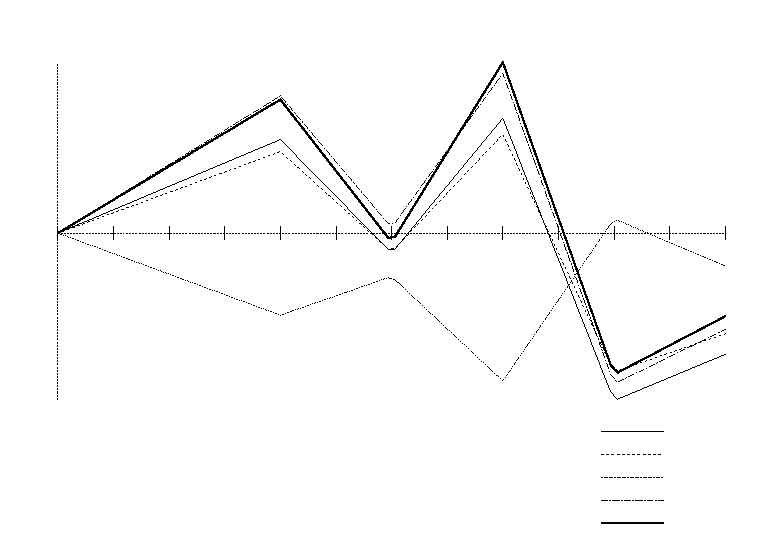
\includegraphics{fig-piecewiseIncome}}%
    \gplfronttext
  \end{picture}%
\endgroup

\caption{\label{fig:piecewiseIncome}Latent variable as a function of
  income with the estimated coefficients}
\end{figure}

\item We refer the reader to \citeasnoun{vij2016and}, who discuss the actual
  added value (or lack thereof) of using latent variables in the
  context of a choice   model. 

\end{itemize}

\clearpage

\appendix

\section{Description of the case study}

This case study deals with the estimation of a mode choice behavior
model for inhabitants in Switzerland using revealed preference data.
The survey was conducted between 2009 and 2010 for CarPostal, the public transport
branch of the Swiss Postal Service. The main purpose of this survey
is to collect data for analyzing the travel behavior of people in
low-density areas, where CarPostal typically serves. A following
study proposes new public transport alternatives according to the respondents'
willingness to pay for these potential services in order to increase
the market share of public transport.


\subsection{Data collection}

The survey covers French and German speaking areas of Switzerland. Questionnaires
were sent to people living in rural area by mail. The respondents
were asked to register all the trips performed during a specified
day. The collected information consists of origin, destination,
cost, travel time, chosen mode and activity at the destination. Moreover, we collected socio-economic information about the respondents and their households.

1124 completed surveys were collected. For each respondent,
cyclic sequences of trips (starting and ending at the same location)
are detected and their main transport mode is identified. The resulting data base includes 1906 sequences of trips linked with psychometric indicators and socio-economic attributes of the respondents. It should be noticed that each observation is a sequence of trips
that starts and ends at home. A respondent may have several sequences of trips 
in a day.

%Some socio-economic characteristics, such as gender, children and age, are also collected.
%The observations in this data set are weighted according to the statistical
%data of Switzerland considering 6 dimensions: presence of driving
%license, gender, education, number of cars in the household, age,
%and number of people in the household. These weights for individuals
%are used for having a weighted average value for the outputs of the
%model, for example cost and time elasticities in this paper, to be
%able to better represent the Swiss population.

\subsection{Variables and descriptive statistics}

The variables are described in Table \ref{tab1}. The attitudinal statements are described in Table \ref{tab:indic}. A summary of descriptive statistics for the main variables is given in Table \ref{tab8}.


Given the presence of missing data (coded as -1) an additional table summarizing the three main affected variables (TripPurpose, ReportedDuration,	age) after removing the missing cases is presented (see Table \ref{tab9}).

\clearpage


\begin{longtable}{||p{4cm}|p{9cm}||}
\caption{\label{tab1} Description of variables}\\
\hline 
\hline 
\textbf{Name} & \textbf{Description}\\
%\tabularnewline
\hline 
ID & Identifier of the respondent who described the trips in the loop.\tabularnewline
\hline 
NbTransf & The total number of transfers performed for all trips of the loop,
using public transport (ranging from 1-9).\tabularnewline
\hline 
TimePT & The duration of the loop performed in public transport (in minutes).\tabularnewline
\hline 
WalkingTimePT & The total walking time in a loop performed in public transports (in minutes).\tabularnewline
\hline 
WaitingTimePT & The total waiting time in a loop performed in public transports (in minutes).\tabularnewline
\hline 
TimeCar & The total duration of a loop made using the car (in minutes).\tabularnewline
\hline 
CostPT & Cost for public transports (full cost to perform the loop). \tabularnewline
\hline 
MarginalCostPT & The total cost of a loop performed in public transports, taking into account the ownership of a seasonal ticket by the respondent. If the respondent has a ``GA'' (full Swiss season ticket), a seasonal ticket for the line or the area, this variable takes value zero. If the respondent has a half-fare travelcard, this variable corresponds to half the cost of the trip by public transport..\tabularnewline
\hline 
CostCarCHF & The total gas cost of a loop performed with the car in CHF.\tabularnewline
\hline 
CostCar & The total gas cost of a loop performed with the car in euros.\tabularnewline
\hline 
TripPurpose & The main purpose of the loop: 1 =Work-related trips; 2 =Work- and leisure-related
trips; 3 =Leisure related trips. -1 represents missing values \tabularnewline
\hline 
TypeCommune & The commune type, based on the Swiss Federal Statistical Office 1 =Centers;
2 =Suburban communes; 3 =High-income communes; 4 =Periurban communes;
5 =Touristic communes; 6 =Industrial and tertiary communes; 7 =Rural
and commuting communes; 8 =Agricultural and mixed communes; 9 =Agricultural
communes\tabularnewline
\hline 
UrbRur & Binary variable, where: 1 =Rural; 2 =Urban.\tabularnewline
\hline 
ClassifCodeLine & Classification of the type of bus lines of the commune: 1 =Center; 2
=Centripetal; 3 =Peripheral; 4 =Feeder.\tabularnewline
\hline
frequency & Categorical variable for the frequency: 1 =Low frequency, $<$ 12 pairs
of trips per day; 2 =Low-middle frequency, 13 - 20 pairs of trips
per day; 3 =Middle-high frequency, 21-30 pairs of trips per day;
4 =High frequency, $>$ 30 pairs of trips per day.\tabularnewline
\hline 
NbTrajects & Number of trips in the loop \tabularnewline
\hline 
Region OR CoderegionCAR & Region where the commune of the respondent is situated. These regions
are defined by CarPostal as follows: 1 =Vaud; 2 =Valais; 3 =Delemont;
4 =Bern; 5 =Basel, Aargau, Olten; 6 =Zurich; 7 =Eastern Switzerland;
8 =Graubunden.\tabularnewline
\hline 
distance\_km & Total distance performed for the loop.\tabularnewline
\hline 
Choice & Choice variable: 0 = public transports (train, bus, tram, etc.); 1
= private modes (car, motorbike, etc.); 2 = soft modes (bike, walk,
etc.).\tabularnewline
\hline 
InVehicleTime & Time spent in (on-board) the transport modes only (discarding walking time and
waiting time), -1 if missing value.\tabularnewline
\hline 
ReportedDuration & Time spent for the whole loop, as reported by the respondent. -1 represents missing values\tabularnewline
\hline 
LangCode & Language of the commune where the survey was conducted: 1 =French;
2 =German.\tabularnewline
\hline 
age & Age of the respondent (in years) -1 represents missing values.\tabularnewline
\hline
DestAct & The main activity at destination: 1 is work, 2 is professional trip, 3 is studying, 4 is shopping, 5 is activity at home, 6 is eating/drinking, 7 is personal business, 8 is driving someone, 9 is cultural activity or sport, 10 is going out (with friends, restaurant, cinema, theater), 11 is other and -1 is missing value. \tabularnewline
\hline
FreqTripHouseh & Frequency of trips related to the household (drive someone, like kids, or shopping), 1 is never, 2 is several times a day, 3 is several times a week, 4 is occasionally, -1 is for missing data and -2 if respondent didn't answer to any opinion questions. \tabularnewline
ModeToSchool & Most often mode used by the respondent to go to school as a kid ($>10$), 1 is car (passenger), 2 is train, 3 is public transport, 4 is walking, 5 is biking, 6 is motorbike, 7 is other, 8 is multiple modes, -1 is for missing data and -2 if respondent didn't answer to any opinion questions. \tabularnewline
\hline 
ResidChild & Main place of residence as a kid ($<18$), 1 is city center (large town), 2 is city center (small town), 3 is suburbs, 4 is suburban town, 5 is country side (village), 6 is countryside (isolated), -1 is for missing data and -2 if respondent didn't answer to any opinion questions. \tabularnewline
\hline 
FreqCarPar & Frequency of the usage of car by the respondent's parents (or adults in charge) during childhood ($<18$), 1 is never, 2 is occasionally, 3 is regularly, 4 is exclusively, -1 is for missing data and -2 if respondent didn't answer to any opinion questions. \tabularnewline
\hline 
FreqTrainPar & Frequency of the usage of train by the respondent's parents (or adults in charge) during childhood ($<18$), 1 is never, 2 is occasionally, 3 is regularly, 4 is exclusively, -1 is for missing data and -2 if respondent didn't answer to any opinion questions. \tabularnewline 
\hline 
FreqOthPar & Frequency of the usage of tram, bus and other public transport (not train) by the respondent's parents (or adults in charge) during childhood ($<18$), 1 is never, 2 is occasionally, 3 is regularly, 4 is exclusively , -1 is for missing data and -2 if respondent didn't answer to any opinion questions. \tabularnewline
\hline
NbHousehold & Number of persons in the household. -1 for missing value. \tabularnewline
\hline 
NbChild & Number of kids ($<15$) in the household. -1 for missing value. \tabularnewline
\hline 
NbCar & Number of cars in the household.-1 for missing value. \tabularnewline
\hline 
NbMoto & Number of motorbikes in the household. -1 for missing value.\tabularnewline
\hline 
NbBicy & Number of bikes in the household. -1 for missing value.\tabularnewline
\hline 
NbBicyChild & Number of bikes for kids in the household. -1 for missing value.\tabularnewline
\hline 
NbComp & Number of computers in the household. -1 for missing value.\tabularnewline
\hline 
NbTV & Number of TVs in the household. -1 for missing value.\tabularnewline
\hline 
Internet & Internet connection, 1 is yes, 2 is no. -1 for missing value.\tabularnewline
\hline 
NewsPaperSubs & Newspaper subscription, 1 is yes, 2 is no. -1 for missing value.\tabularnewline
\hline 
NbCellPhones & Number of cell phones in the household (total). -1 for missing value.\tabularnewline
\hline 
NbSmartPhone & Number of smartphones in the household (total). -1 for missing value.\tabularnewline
\hline 
HouseType & House type, 1 is individual house (or terraced house), 2 is apartment (and other types of multi-family residential), 3 is independent room (subletting). -1 for missing value.\tabularnewline
\hline 
OwnHouse & Do you own the place where you are living? 1 is yes, 2 is no. -1 for missing value.\tabularnewline
\hline 
NbRoomsHouse & Number of rooms is your house. -1 for missing value.\tabularnewline
\hline 
YearsInHouse & Number of years spent in the current house. -1 for missing value.\tabularnewline
\hline 
Income & Net monthly income of the household in CHF. 1 is less than 2500, 2 is from 2501 to 4000, 3 is from 4001 to 6000, 4 is from 6001 to 8000, 5 is from 8001 to 10'000 and 6 is more than 10'001. -1 for missing value.\tabularnewline
\hline 
Gender & Gender of the respondent, 1 is man, 2 is woman. -1 for missing value.\tabularnewline
\hline 
BirthYear & Year of birth of the respondent. -1 for missing value.\tabularnewline
\hline 
Mothertongue & Mothertongue. 1 for German or Swiss German, 2 for french, 3 for other, -1 for missing value.\tabularnewline
\hline
FamilSitu & Familiar situation: 1 is single, 2 is in a couple without children, 3 is in a couple with children, 4 is single with your own children, 5 is in a colocation, 6 is with your parents and 7 is for other situations. -1 for missing values.\tabularnewline
\hline
OccupStat &What is you occupational status? 1 is for full-time paid
professional activity, 2 for partial-time paid professional activity,
3 for searching a job, 4 for occasional employment, 5 for no paid job,
6 for homemaker, 7 for disability leave, 8 for student and 9 for retired. -1 for missing values. \tabularnewline
\hline
SocioProfCat & To which of the following socio-professional categories do you belong? 1 is for top managers, 2 for intellectual professions, 3 for freelancers, 4 for intermediate professions, 5 for artisans and salespersons, 6 for employees, 7 for workers and 8 for others. -1 for missing values.\tabularnewline
\hline
Education &Highest education achieved. As mentioned by Wikipedia in English: "The education system in Switzerland is very diverse, because the constitution of Switzerland delegates the authority for the school system mainly to the cantons. The Swiss constitution sets the foundations, namely that primary school is obligatory for every child and is free in public schools and that the confederation can run or support universities." (source: \lstinline|http://en.wikipedia.org/wiki/Education_in_Switzerland|, accessed April 16, 2013). It is thus difficult to translate the survey that was originally in French and German. The possible answers in the survey are:
1. Unfinished compulsory education: education is compulsory in Switzerland but pupils may finish it at the legal age without succeeding the final exam.
2. Compulsory education with diploma
3. Vocational education: a three or four-year period of training both in a company and following theoretical courses. Ends with a diploma called "Certificat f\'ed\'eral de capacit\'e" (i.e., "professional baccalaureate")
4. A 3-year generalist school giving access to teaching school, nursing schools, social work school, universities of applied sciences or vocational education (sometime in less than the normal number of years). It does not give access to universities in Switzerland
5. High school: ends with the general baccalaureate exam. The general baccalaureate gives access automatically to universities.
6. Universities of applied sciences, teaching schools, nursing schools, social work schools: ends with a Bachelor and sometimes a Master, mostly focus on vocational training
7. Universities and institutes of technology: ends with an academic Bachelor and in most cases an academic Master
8. PhD thesis \tabularnewline
\hline
HalfFareST & Is equal to 1 if the respondent has a half-fare travelcard and to 2 if not.\tabularnewline
\hline
%X338 & Duration of the half-fare travelcard (1, 2, 3 years).\tabularnewline
%\hline
LineRelST & Is equal to 1 if the respondent has a line-related season ticket and 2 if not.\tabularnewline
\hline 
GenAbST & Is equal to 1 if the respondent has a GA (full Swiss season ticket) and 2 if not.\tabularnewline
\hline 
AreaRelST & Is equal to 1 if the respondent has an area-related season ticket and 2 if not.\tabularnewline
\hline
OtherST & Is equal to 1 if the respondent has a season ticket that was is not in the list and 2 if not.\tabularnewline
\hline 
CarAvail & Represents the availability of a car for the respondent: 1 is always, 2 is sometime, 3 is never. -1 for missing value.\tabularnewline
\hline 
\hline 
\end{longtable}

\clearpage

\begin{longtable}{||p{4cm}|p{9cm}||}
\caption{\label{tab:indic}Attitude questions. Coding: 1= strongly disagree, 2=disagree,
  3=neutral, 4= agree, 5= strongly agree, 6=not applicable, -1=
  missing value, -2= all answers to attitude questions missing} \\
\hline 
\hline 
\textbf{Name} & \textbf{Description}\\
%\tabularnewline
\hline 
Envir01 & Fuel price should be increased to reduce congestion and air pollution. \tabularnewline
\hline 
Envir02 & More public transportation is needed, even if taxes are set to pay the additional costs.\tabularnewline
\hline 
Envir03 & Ecology disadvantages minorities and small businesses.\tabularnewline
\hline 
Envir04 & People and employment are more important than the environment.\tabularnewline
\hline 
Envir05 & I am concerned about global warming.\tabularnewline
\hline 
Envir06 & Actions and decision making are needed to limit greenhouse gas emissions.\tabularnewline
\hline 
Mobil01 & My trip is a useful transition between home and work.\tabularnewline
\hline 
Mobil02 & The trip I must do interferes with other things I would like to do. \tabularnewline
\hline 
Mobil03 & I use the time of my trip in a productive way.\tabularnewline
\hline 
Mobil04 & Being stuck in traffic bores me.\tabularnewline
\hline 
Mobil05 & I reconsider frequently my mode choice.\tabularnewline
\hline 
Mobil06 & I use my current mean of transport mode because I have no alternative.\tabularnewline
\hline 
Mobil07 & In general, for my activities, I always have a usual mean of transport.\tabularnewline
\hline 
Mobil08 & I do not feel comfortable when I travel close to people I do not know.\tabularnewline
\hline 
Mobil09 & Taking the bus helps making the city more comfortable and welcoming.\tabularnewline
\hline 
Mobil10 & It is difficult to take the public transport when I travel with my children.\tabularnewline
\hline 
Mobil11 & It is difficult to take the public transport when I carry bags or luggage.\tabularnewline
\hline 
Mobil12 & It is very important to have a beautiful car.\tabularnewline
\hline 
Mobil13 & With my car I can go wherever and whenever.\tabularnewline
\hline 
Mobil14 & When I take the car I know I will be on time.\tabularnewline
\hline 
Mobil15 & I do not like looking for a parking place. \tabularnewline
\hline 
Mobil16 & I do not like changing the mean of transport when I am traveling.\tabularnewline
\hline 
Mobil17 & If I use public transportation I have to cancel certain activities I would have done if I had taken the car. \tabularnewline
\hline 
Mobil18 & CarPostal bus schedules are sometimes difficult to understand.\tabularnewline
\hline 
Mobil19 & I know very well which bus/train I have to take to go where I want to.\tabularnewline
\hline 
Mobil20 & I know by heart the schedules of the public transports I regularly use. \tabularnewline
\hline 
Mobil21 & I can rely on my family to drive me if needed\tabularnewline
\hline 
Mobil22 & When I am in a town I don't know I feel strongly disoriented\tabularnewline
\hline 
Mobil23 & I use the internet to check the schedules and the departure times of buses and trains.\tabularnewline
\hline 
Mobil24 & I have always used public transports all my life\tabularnewline
\hline 
Mobil25 & When I was young my parents took me to all my activities\tabularnewline
\hline 
Mobil26 & I know some drivers of the public transports that I use \tabularnewline
\hline 
Mobil27 & I think it is important to have the option to talk to the drivers of public transports.\tabularnewline
\hline 
ResidCh01 & I like living in a neighborhood where a lot of things happen. \tabularnewline
\hline 
ResidCh02 & The accessibility and mobility conditions are important for the choice of housing. \tabularnewline
\hline 
ResidCh03 & Most of my friends live in the same region I live in.\tabularnewline
\hline 
ResidCh04 & I would like to have access to more services or activities. \tabularnewline
\hline 
ResidCh05 & I would like to live in the city center of a big city.\tabularnewline
\hline 
ResidCh06 & I would like to live in a town situated in the outskirts of a city. \tabularnewline
\hline 
ResidCh07 & I would like to live in the countryside.\tabularnewline
\hline 
LifSty01 & I always choose the best products regardless of price. \tabularnewline
\hline 
LifSty02 & I always try to find the cheapest alternative. \tabularnewline
\hline 
LifSty03 & I can ask for services in my neighborhood without problems. \tabularnewline
\hline 
LifSty04 & I would like to spend more time with my family and friends. \tabularnewline
\hline 
LifSty05 & Sometimes I would like to take a day off .\tabularnewline
\hline 
LifSty06 & I can recognize the social status of other travelers by looking at their cars.\tabularnewline
\hline 
LifSty07 & The pleasure of having something beautiful consists in showing it. \tabularnewline
\hline 
LifSty08 & For me the car is only a practical way to move. \tabularnewline
\hline 
LifSty09 & I would like to spend more time working.\tabularnewline
\hline 
LifSty10 & I do not like to be in the same place for too long.\tabularnewline
\hline 
LifSty11 & I always plan my activities well in advance \tabularnewline
\hline 
LifSty12 & I like to experiment new or different situations\tabularnewline
\hline 
LifSty13 & I am not afraid of unknown people\tabularnewline
\hline 
LifSty14 & My schedule is rather regular.\tabularnewline
\hline 
\hline 
\end{longtable}



\begin{sidewaystable}[htbp]
\caption{\label{tab8} Descriptive statistics of the main variables (no data excluded) }
\vspace{0.2cm}
\begin{tabular}{||l|c|c|c|c|c|c|c||}
\hline
 & \multicolumn{1}{l|}{nbr. cases} & \multicolumn{1}{l|}{nbr. null} & \multicolumn{1}{l|}{min} & \multicolumn{1}{l|}{max} & \multicolumn{1}{l|}{median} & \multicolumn{1}{l|}{mean} & \multicolumn{1}{l|}{std.dev} \\ \hline
age & 1906 & 0 & -1 & 88 & 47 & 46.48 & 18.57 \\ \hline
Choice & 1906 & 536 & 0 & 2 & 1 & 0.78 & 0.54 \\ \hline
TypeCommune & 1906 & 0 & 1 & 9 & 6 & 5.39 & 1.99 \\ \hline
UrbRur & 1906 & 0 & 1 & 2 & 2 & 1.51 & 0.5 \\ \hline
ClassifCodeLine & 1906 & 0 & 1 & 4 & 4 & 3.17 & 0.97 \\ \hline
LangCode & 1906 & 0 & 1 & 2 & 2 & 1.74 & 0.44 \\ \hline
CoderegionCAR & 1906 & 0 & 1 & 8 & 5 & 4.58 & 2.08 \\ \hline
CostCarCHF & 1906 & 5 & 0 & 67.65 & 2.98 & 5.76 & 8.34 \\ \hline
distance\_km & 1906 & 1 & 0 & 519 & 18.75 & 40.38 & 62.6 \\ \hline
TimeCar & 1906 & 28 & 0 & 494 & 26 & 40.68 & 47.61 \\ \hline
TimePT & 1906 & 7 & 0 & 745 & 85 & 107.88 & 86.52 \\ \hline
frequency & 1906 & 0 & 1 & 4 & 3 & 2.84 & 1.09 \\ \hline
ID & 1906 & 0 & 10350017 & 96040538 & 44690042 & 45878800 & 23846908 \\ \hline
InVehicleTime & 1906 & 66 & -128 & 631 & 40.5 & 55.13 & 57.78 \\ \hline
MarginalCostPT & 1906 & 270 & 0 & 230 & 5.6 & 11.11 & 16.13 \\ \hline
NbTrajects & 1906 & 0 & 1 & 9 & 2 & 2.04 & 1.05 \\ \hline
NbTransf & 1906 & 644 & 0 & 14 & 2 & 2.01 & 2.17 \\ \hline
Region & 1906 & 0 & 1 & 8 & 5 & 4.58 & 2.08 \\ \hline
ReportedDuration & 1906 & 3 & -1 & 855 & 35 & 57.73 & 72.47 \\ \hline
TripPurpose & 1906 & 0 & -1 & 3 & 2 & 1.94 & 1.18 \\ \hline
WaitingTimePT & 1906 & 693 & 0 & 392 & 5 & 13.13 & 22.07 \\ \hline
WalkingTimePT & 1906 & 17 & 0 & 213 & 33 & 39.63 & 28 \\ \hline
\end{tabular}
\end{sidewaystable}



\begin{table}[htbp]
\caption{\label{tab9}
Descriptive statistics of the main variables affected by missing data (observations with -1 excluded)}
\vspace{0.2cm}
\begin{tabular}{|l|r|r|r|r|r|r|r|}
\hline
\multicolumn{1}{|r|}{} & \multicolumn{1}{l|}{nbr. cases} & \multicolumn{1}{l|}{nbr.null} &  \multicolumn{1}{l|}{min} & \multicolumn{1}{l|}{max} & \multicolumn{1}{l|}{median} & \multicolumn{1}{l|}{mean} & \multicolumn{1}{l|}{std.dev} \\ \hline
age & 1791 & 0  & 16 & 88 & 48 & 49.53 & 14.59 \\ \hline
ReportedDuration & 1835 & 3 & 0 & 855 & 37 & 60 & 72.92 \\ \hline
TripPurpose & 1783 & 0  & 1 & 3 & 3 & 2.14 & 0.92 \\ \hline
\end{tabular}
\end{table}

\clearpage

\section{Complete specification files}

\subsection{\lstinline+00factorAnalysis.py+}
\label{sec:factoranalysis}
\begin{lstlisting}[style=numbers]
import pandas as pd
import numpy as np

# The following package can be installed using
# pip install factor_analyzer
# See https://github.com/EducationalTestingService/factor_analyzer
from factor_analyzer import FactorAnalyzer


# We first extract the columns containing the indicators
indicators = pd.read_table("optima.dat",usecols=["Envir01",
        "Envir02",
	"Envir03",
	"Envir04",
	"Envir05",
	"Envir06",
	"Mobil01",
	"Mobil02",
	"Mobil03",
	"Mobil04",
	"Mobil05",
	"Mobil06",
	"Mobil07",
	"Mobil08",
	"Mobil09",
	"Mobil10",
	"Mobil11",
	"Mobil12",
	"Mobil13",
	"Mobil14",
	"Mobil15",
	"Mobil16",
	"Mobil17",
	"Mobil18",
	"Mobil19",
	"Mobil20",
	"Mobil21",
	"Mobil22",
	"Mobil23",
	"Mobil24",
	"Mobil25",
	"Mobil26",
	"Mobil27",
	"ResidCh01",
	"ResidCh02",
	"ResidCh03",
	"ResidCh04",
	"ResidCh05",
	"ResidCh06",
	"ResidCh07",
	"LifSty01",
	"LifSty02",
	"LifSty03",
	"LifSty04",
	"LifSty05",
	"LifSty06",
	"LifSty07",
	"LifSty08",
	"LifSty09",
	"LifSty10",
	"LifSty11",
	"LifSty12",
	"LifSty13",
	"LifSty14"])

# Negative values are missing values. 
indicators[indicators <= 0] = np.nan
indicators = indicators.dropna(axis = 0, how = 'any') 

fa = FactorAnalyzer()
fa.analyze(indicators,3,rotation='varimax')


labeledResults = pd.DataFrame(fa.loadings)
filter = (labeledResults <= 0.4) & (labeledResults >= -0.4)
labeledResults[filter] = ''
print(labeledResults)
\end{lstlisting}

\subsection{\lstinline$01oneLatentRegression.py$}
\label{sec:01oneLatentRegression}
\begin{lstlisting}[style=numbers]
import pandas as pd
import numpy as np
import biogeme.database as db
import biogeme.biogeme as bio
from biogeme.models import piecewise
import biogeme.loglikelihood as ll


pandas = pd.read_table("optima.dat")
database = db.Database("optima",pandas)

from headers import *

exclude = (Choice == -1.0)
database.remove(exclude)


# Piecewise linear definition of income

ScaledIncome = DefineVariable('ScaledIncome',\
                              CalculatedIncome / 1000,database)

thresholds = [4,6,8,10]
ContIncome = piecewise(ScaledIncome,thresholds)
ContIncome_0_4000 = ContIncome[0]
ContIncome_4000_6000 = ContIncome[1]
ContIncome_6000_8000 = ContIncome[2]
ContIncome_8000_10000 = ContIncome[3]
ContIncome_10000_more = ContIncome[4]

age_65_more = DefineVariable('age_65_more',age >= Numeric(65),database)
moreThanOneCar = DefineVariable('moreThanOneCar',NbCar > 1,database)
moreThanOneBike = DefineVariable('moreThanOneBike',NbBicy > 1,database)
individualHouse = DefineVariable('individualHouse',\
                                 HouseType == 1,database)
male = DefineVariable('male',Gender == 1,database)
haveChildren = DefineVariable('haveChildren',\
                              ((FamilSitu == 3)+(FamilSitu == 4)) > 0,database)
haveGA = DefineVariable('haveGA',GenAbST == 1,database)
highEducation = DefineVariable('highEducation', Education >= 6,database)

### Coefficients
coef_intercept = Beta('coef_intercept',0.0,None,None,0)
coef_age_65_more = Beta('coef_age_65_more',0.0,None,None,0)
coef_age_unknown = Beta('coef_age_unknown',0.0,None,None,0)
coef_haveGA = Beta('coef_haveGA',0.0,None,None,0)
coef_ContIncome_0_4000 = \
 Beta('coef_ContIncome_0_4000',0.0,None,None,0)
coef_ContIncome_4000_6000 = \
 Beta('coef_ContIncome_4000_6000',0.0,None,None,0)
coef_ContIncome_6000_8000 = \
 Beta('coef_ContIncome_6000_8000',0.0,None,None,0)
coef_ContIncome_8000_10000 = \
 Beta('coef_ContIncome_8000_10000',0.0,None,None,0)
coef_ContIncome_10000_more = \
 Beta('coef_ContIncome_10000_more',0.0,None,None,0)
coef_moreThanOneCar = \
 Beta('coef_moreThanOneCar',0.0,None,None,0)
coef_moreThanOneBike = \
 Beta('coef_moreThanOneBike',0.0,None,None,0)
coef_individualHouse = \
 Beta('coef_individualHouse',0.0,None,None,0)
coef_male = Beta('coef_male',0.0,None,None,0)
coef_haveChildren = Beta('coef_haveChildren',0.0,None,None,0)
coef_highEducation = Beta('coef_highEducation',0.0,None,None,0)

### Latent variable: structural equation

# Note that the expression must be on a single line. In order to 
# write it across several lines, each line must terminate with 
# the \ symbol

CARLOVERS = \
coef_intercept +\
coef_age_65_more * age_65_more +\
coef_ContIncome_0_4000 * ContIncome_0_4000 +\
coef_ContIncome_4000_6000 * ContIncome_4000_6000 +\
coef_ContIncome_6000_8000 * ContIncome_6000_8000 +\
coef_ContIncome_8000_10000 * ContIncome_8000_10000 +\
coef_ContIncome_10000_more * ContIncome_10000_more +\
coef_moreThanOneCar * moreThanOneCar +\
coef_moreThanOneBike * moreThanOneBike +\
coef_individualHouse * individualHouse +\
coef_male * male +\
coef_haveChildren * haveChildren +\
coef_haveGA * haveGA +\
coef_highEducation * highEducation

sigma_s = Beta('sigma_s',1,0.001,None,1)

### Measurement equations

INTER_Envir01 = Beta('INTER_Envir01',0,None,None,1)
INTER_Envir02 = Beta('INTER_Envir02',0,None,None,0)
INTER_Envir03 = Beta('INTER_Envir03',0,None,None,0)
INTER_Mobil11 = Beta('INTER_Mobil11',0,None,None,0)
INTER_Mobil14 = Beta('INTER_Mobil14',0,None,None,0)
INTER_Mobil16 = Beta('INTER_Mobil16',0,None,None,0)
INTER_Mobil17 = Beta('INTER_Mobil17',0,None,None,0)

B_Envir01_F1 = Beta('B_Envir01_F1',-1,None,None,1)
B_Envir02_F1 = Beta('B_Envir02_F1',-1,None,None,0)
B_Envir03_F1 = Beta('B_Envir03_F1',1,None,None,0)
B_Mobil11_F1 = Beta('B_Mobil11_F1',1,None,None,0)
B_Mobil14_F1 = Beta('B_Mobil14_F1',1,None,None,0)
B_Mobil16_F1 = Beta('B_Mobil16_F1',1,None,None,0)
B_Mobil17_F1 = Beta('B_Mobil17_F1',1,None,None,0)



MODEL_Envir01 = INTER_Envir01 + B_Envir01_F1 * CARLOVERS
MODEL_Envir02 = INTER_Envir02 + B_Envir02_F1 * CARLOVERS
MODEL_Envir03 = INTER_Envir03 + B_Envir03_F1 * CARLOVERS
MODEL_Mobil11 = INTER_Mobil11 + B_Mobil11_F1 * CARLOVERS
MODEL_Mobil14 = INTER_Mobil14 + B_Mobil14_F1 * CARLOVERS
MODEL_Mobil16 = INTER_Mobil16 + B_Mobil16_F1 * CARLOVERS
MODEL_Mobil17 = INTER_Mobil17 + B_Mobil17_F1 * CARLOVERS

SIGMA_STAR_Envir01 = Beta('SIGMA_STAR_Envir01',10,0.001,None,0)
SIGMA_STAR_Envir02 = Beta('SIGMA_STAR_Envir02',10,0.001,None,0)
SIGMA_STAR_Envir03 = Beta('SIGMA_STAR_Envir03',10,0.001,None,0)
SIGMA_STAR_Mobil11 = Beta('SIGMA_STAR_Mobil11',10,0.001,None,0)
SIGMA_STAR_Mobil14 = Beta('SIGMA_STAR_Mobil14',10,0.001,None,0)
SIGMA_STAR_Mobil16 = Beta('SIGMA_STAR_Mobil16',10,0.001,None,0)
SIGMA_STAR_Mobil17 = Beta('SIGMA_STAR_Mobil17',10,0.001,None,0)


F = {}
F['Envir01'] = Elem({0:0, \
 1:ll.loglikelihoodregression(Envir01,MODEL_Envir01,SIGMA_STAR_Envir01)},\
  (Envir01 > 0)*(Envir01 < 6))
F['Envir02'] = Elem({0:0, \
 1:ll.loglikelihoodregression(Envir02,MODEL_Envir02,SIGMA_STAR_Envir02)},\
  (Envir02 > 0)*(Envir02 < 6))
F['Envir03'] = Elem({0:0, \
 1:ll.loglikelihoodregression(Envir03,MODEL_Envir03,SIGMA_STAR_Envir03)},\
  (Envir03 > 0)*(Envir03 < 6))
F['Mobil11'] = Elem({0:0, \
 1:ll.loglikelihoodregression(Mobil11,MODEL_Mobil11,SIGMA_STAR_Mobil11)},\
  (Mobil11 > 0)*(Mobil11 < 6))
F['Mobil14'] = Elem({0:0, \
 1:ll.loglikelihoodregression(Mobil14,MODEL_Mobil14,SIGMA_STAR_Mobil14)},\
  (Mobil14 > 0)*(Mobil14 < 6))
F['Mobil16'] = Elem({0:0, \
 1:ll.loglikelihoodregression(Mobil16,MODEL_Mobil16,SIGMA_STAR_Mobil16)},\
  (Mobil16 > 0)*(Mobil16 < 6))
F['Mobil17'] = Elem({0:0, \
 1:ll.loglikelihoodregression(Mobil17,MODEL_Mobil17,SIGMA_STAR_Mobil17)},\
  (Mobil17 > 0)*(Mobil17 < 6))

loglike = bioMultSum(F)

biogeme  = bio.BIOGEME(database,loglike)
biogeme.modelName = "01oneLatentRegression"
results = biogeme.estimate()
print(f"Estimated betas: {len(results.data.betaValues)}")
print(f"final log likelihood: {results.data.logLike:.3f}")
print(f"Output file: {results.data.htmlFileName}")
results.writeLaTeX()
print(f"LaTeX file: {results.data.latexFileName}")
\end{lstlisting}


\subsection{\lstinline$02oneLatentOrdered.py$}
\label{sec:02oneLatentOrdered}

\begin{lstlisting}[style=numbers]
import pandas as pd
import numpy as np
import biogeme.database as db
import biogeme.biogeme as bio
#import biogeme.models as models
import biogeme.loglikelihood as ll

pandas = pd.read_table("optima.dat")
database = db.Database("optima",pandas)

from headers import *

exclude = (Choice == -1.0)
database.remove(exclude)



### Variables

ScaledIncome = DefineVariable('ScaledIncome',\
                              CalculatedIncome / 1000,database)
ContIncome_0_4000 = DefineVariable('ContIncome_0_4000',\
                                   bioMin(ScaledIncome,4),database)
ContIncome_4000_6000 = DefineVariable('ContIncome_4000_6000',\
                                      bioMax(0,bioMin(ScaledIncome-4,2)),database)
ContIncome_6000_8000 = DefineVariable('ContIncome_6000_8000',\
                                      bioMax(0,bioMin(ScaledIncome-6,2)),database)
ContIncome_8000_10000 = DefineVariable('ContIncome_8000_10000',\
                                       bioMax(0,bioMin(ScaledIncome-8,2)),database)
ContIncome_10000_more = DefineVariable('ContIncome_10000_more',\
                                       bioMax(0,ScaledIncome-10),database)

age_65_more = DefineVariable('age_65_more',age >= Numeric(65),database)
moreThanOneCar = DefineVariable('moreThanOneCar',NbCar > 1,database)
moreThanOneBike = DefineVariable('moreThanOneBike',NbBicy > 1,database)
individualHouse = DefineVariable('individualHouse',\
                                 HouseType == 1,database)
male = DefineVariable('male',Gender == 1,database)
haveChildren = DefineVariable('haveChildren',\
                              ((FamilSitu == 3)+(FamilSitu == 4)) > 0,database)
haveGA = DefineVariable('haveGA',GenAbST == 1,database)
highEducation = DefineVariable('highEducation', Education >= 6,database)

### Coefficients
coef_intercept = Beta('coef_intercept',0.0,None,None,0 )
coef_age_65_more = Beta('coef_age_65_more',0.0,None,None,0 )
coef_haveGA = Beta('coef_haveGA',0.0,None,None,0 )
coef_ContIncome_0_4000 = \
 Beta('coef_ContIncome_0_4000',0.0,None,None,0 )
coef_ContIncome_4000_6000 = \
 Beta('coef_ContIncome_4000_6000',0.0,None,None,0 )
coef_ContIncome_6000_8000 = \
 Beta('coef_ContIncome_6000_8000',0.0,None,None,0 )
coef_ContIncome_8000_10000 = \
 Beta('coef_ContIncome_8000_10000',0.0,None,None,0 )
coef_ContIncome_10000_more = \
 Beta('coef_ContIncome_10000_more',0.0,None,None,0 )
coef_moreThanOneCar = \
 Beta('coef_moreThanOneCar',0.0,None,None,0 )
coef_moreThanOneBike = \
 Beta('coef_moreThanOneBike',0.0,None,None,0 )
coef_individualHouse = \
 Beta('coef_individualHouse',0.0,None,None,0 )
coef_male = Beta('coef_male',0.0,None,None,0 )
coef_haveChildren = Beta('coef_haveChildren',0.0,None,None,0 )
coef_highEducation = Beta('coef_highEducation',0.0,None,None,0 )

### Latent variable: structural equation

# Note that the expression must be on a single line. In order to 
# write it across several lines, each line must terminate with 
# the \ symbol

CARLOVERS = \
coef_intercept +\
coef_age_65_more * age_65_more +\
coef_ContIncome_0_4000 * ContIncome_0_4000 +\
coef_ContIncome_4000_6000 * ContIncome_4000_6000 +\
coef_ContIncome_6000_8000 * ContIncome_6000_8000 +\
coef_ContIncome_8000_10000 * ContIncome_8000_10000 +\
coef_ContIncome_10000_more * ContIncome_10000_more +\
coef_moreThanOneCar * moreThanOneCar +\
coef_moreThanOneBike * moreThanOneBike +\
coef_individualHouse * individualHouse +\
coef_male * male +\
coef_haveChildren * haveChildren +\
coef_haveGA * haveGA +\
coef_highEducation * highEducation


### Measurement equations

INTER_Envir01 = Beta('INTER_Envir01',0,None,None,1)
INTER_Envir02 = Beta('INTER_Envir02',0.0,None,None,0 )
INTER_Envir03 = Beta('INTER_Envir03',0.0,None,None,0 )
INTER_Mobil11 = Beta('INTER_Mobil11',0.0,None,None,0 )
INTER_Mobil14 = Beta('INTER_Mobil14',0.0,None,None,0 )
INTER_Mobil16 = Beta('INTER_Mobil16',0.0,None,None,0 )
INTER_Mobil17 = Beta('INTER_Mobil17',0.0,None,None,0 )

B_Envir01_F1 = Beta('B_Envir01_F1',-1,None,None,1)
B_Envir02_F1 = Beta('B_Envir02_F1',0.0,None,None,0 )
B_Envir03_F1 = Beta('B_Envir03_F1',0.0,None,None,0 )
B_Mobil11_F1 = Beta('B_Mobil11_F1',0.0,None,None,0 )
B_Mobil14_F1 = Beta('B_Mobil14_F1',0.0,None,None,0 )
B_Mobil16_F1 = Beta('B_Mobil16_F1',0.0,None,None,0 )
B_Mobil17_F1 = Beta('B_Mobil17_F1',0.0,None,None,0 )



MODEL_Envir01 = INTER_Envir01 + B_Envir01_F1 * CARLOVERS
MODEL_Envir02 = INTER_Envir02 + B_Envir02_F1 * CARLOVERS
MODEL_Envir03 = INTER_Envir03 + B_Envir03_F1 * CARLOVERS
MODEL_Mobil11 = INTER_Mobil11 + B_Mobil11_F1 * CARLOVERS
MODEL_Mobil14 = INTER_Mobil14 + B_Mobil14_F1 * CARLOVERS
MODEL_Mobil16 = INTER_Mobil16 + B_Mobil16_F1 * CARLOVERS
MODEL_Mobil17 = INTER_Mobil17 + B_Mobil17_F1 * CARLOVERS

SIGMA_STAR_Envir01 = Beta('SIGMA_STAR_Envir01',1,None,None,1)
SIGMA_STAR_Envir02 = Beta('SIGMA_STAR_Envir02',1.0,None,None,0 )
SIGMA_STAR_Envir03 = Beta('SIGMA_STAR_Envir03',1.0,None,None,0 )
SIGMA_STAR_Mobil11 = Beta('SIGMA_STAR_Mobil11',1.0,None,None,0 )
SIGMA_STAR_Mobil14 = Beta('SIGMA_STAR_Mobil14',1.0,None,None,0 )
SIGMA_STAR_Mobil16 = Beta('SIGMA_STAR_Mobil16',1.0,None,None,0 )
SIGMA_STAR_Mobil17 = Beta('SIGMA_STAR_Mobil17',1.0,None,None,0 )

delta_1 = Beta('delta_1',0.1,0,10,0 )
delta_2 = Beta('delta_2',0.2,0,10,0 )
tau_1 = -delta_1 - delta_2
tau_2 = -delta_1 
tau_3 = delta_1
tau_4 = delta_1 + delta_2

Envir01_tau_1 = (tau_1-MODEL_Envir01) / SIGMA_STAR_Envir01
Envir01_tau_2 = (tau_2-MODEL_Envir01) / SIGMA_STAR_Envir01
Envir01_tau_3 = (tau_3-MODEL_Envir01) / SIGMA_STAR_Envir01
Envir01_tau_4 = (tau_4-MODEL_Envir01) / SIGMA_STAR_Envir01
IndEnvir01 = {
    1: bioNormalCdf(Envir01_tau_1),
    2: bioNormalCdf(Envir01_tau_2)-bioNormalCdf(Envir01_tau_1),
    3: bioNormalCdf(Envir01_tau_3)-bioNormalCdf(Envir01_tau_2),
    4: bioNormalCdf(Envir01_tau_4)-bioNormalCdf(Envir01_tau_3),
    5: 1-bioNormalCdf(Envir01_tau_4),
    6: 1.0,
    -1: 1.0,
    -2: 1.0
}

P_Envir01 = Elem(IndEnvir01, Envir01)


Envir02_tau_1 = (tau_1-MODEL_Envir02) / SIGMA_STAR_Envir02
Envir02_tau_2 = (tau_2-MODEL_Envir02) / SIGMA_STAR_Envir02
Envir02_tau_3 = (tau_3-MODEL_Envir02) / SIGMA_STAR_Envir02
Envir02_tau_4 = (tau_4-MODEL_Envir02) / SIGMA_STAR_Envir02
IndEnvir02 = {
    1: bioNormalCdf(Envir02_tau_1),
    2: bioNormalCdf(Envir02_tau_2)-bioNormalCdf(Envir02_tau_1),
    3: bioNormalCdf(Envir02_tau_3)-bioNormalCdf(Envir02_tau_2),
    4: bioNormalCdf(Envir02_tau_4)-bioNormalCdf(Envir02_tau_3),
    5: 1-bioNormalCdf(Envir02_tau_4),
    6: 1.0,
    -1: 1.0,
    -2: 1.0
}

P_Envir02 = Elem(IndEnvir02, Envir02)

Envir03_tau_1 = (tau_1-MODEL_Envir03) / SIGMA_STAR_Envir03
Envir03_tau_2 = (tau_2-MODEL_Envir03) / SIGMA_STAR_Envir03
Envir03_tau_3 = (tau_3-MODEL_Envir03) / SIGMA_STAR_Envir03
Envir03_tau_4 = (tau_4-MODEL_Envir03) / SIGMA_STAR_Envir03
IndEnvir03 = {
    1: bioNormalCdf(Envir03_tau_1),
    2: bioNormalCdf(Envir03_tau_2)-bioNormalCdf(Envir03_tau_1),
    3: bioNormalCdf(Envir03_tau_3)-bioNormalCdf(Envir03_tau_2),
    4: bioNormalCdf(Envir03_tau_4)-bioNormalCdf(Envir03_tau_3),
    5: 1-bioNormalCdf(Envir03_tau_4),
    6: 1.0,
    -1: 1.0,
    -2: 1.0
}

P_Envir03 = Elem(IndEnvir03, Envir03)

Mobil11_tau_1 = (tau_1-MODEL_Mobil11) / SIGMA_STAR_Mobil11
Mobil11_tau_2 = (tau_2-MODEL_Mobil11) / SIGMA_STAR_Mobil11
Mobil11_tau_3 = (tau_3-MODEL_Mobil11) / SIGMA_STAR_Mobil11
Mobil11_tau_4 = (tau_4-MODEL_Mobil11) / SIGMA_STAR_Mobil11
IndMobil11 = {
    1: bioNormalCdf(Mobil11_tau_1),
    2: bioNormalCdf(Mobil11_tau_2)-bioNormalCdf(Mobil11_tau_1),
    3: bioNormalCdf(Mobil11_tau_3)-bioNormalCdf(Mobil11_tau_2),
    4: bioNormalCdf(Mobil11_tau_4)-bioNormalCdf(Mobil11_tau_3),
    5: 1-bioNormalCdf(Mobil11_tau_4),
    6: 1.0,
    -1: 1.0,
    -2: 1.0
}

P_Mobil11 = Elem(IndMobil11, Mobil11)

Mobil14_tau_1 = (tau_1-MODEL_Mobil14) / SIGMA_STAR_Mobil14
Mobil14_tau_2 = (tau_2-MODEL_Mobil14) / SIGMA_STAR_Mobil14
Mobil14_tau_3 = (tau_3-MODEL_Mobil14) / SIGMA_STAR_Mobil14
Mobil14_tau_4 = (tau_4-MODEL_Mobil14) / SIGMA_STAR_Mobil14
IndMobil14 = {
    1: bioNormalCdf(Mobil14_tau_1),
    2: bioNormalCdf(Mobil14_tau_2)-bioNormalCdf(Mobil14_tau_1),
    3: bioNormalCdf(Mobil14_tau_3)-bioNormalCdf(Mobil14_tau_2),
    4: bioNormalCdf(Mobil14_tau_4)-bioNormalCdf(Mobil14_tau_3),
    5: 1-bioNormalCdf(Mobil14_tau_4),
    6: 1.0,
    -1: 1.0,
    -2: 1.0
}

P_Mobil14 = Elem(IndMobil14, Mobil14)

Mobil16_tau_1 = (tau_1-MODEL_Mobil16) / SIGMA_STAR_Mobil16
Mobil16_tau_2 = (tau_2-MODEL_Mobil16) / SIGMA_STAR_Mobil16
Mobil16_tau_3 = (tau_3-MODEL_Mobil16) / SIGMA_STAR_Mobil16
Mobil16_tau_4 = (tau_4-MODEL_Mobil16) / SIGMA_STAR_Mobil16
IndMobil16 = {
    1: bioNormalCdf(Mobil16_tau_1),
    2: bioNormalCdf(Mobil16_tau_2)-bioNormalCdf(Mobil16_tau_1),
    3: bioNormalCdf(Mobil16_tau_3)-bioNormalCdf(Mobil16_tau_2),
    4: bioNormalCdf(Mobil16_tau_4)-bioNormalCdf(Mobil16_tau_3),
    5: 1-bioNormalCdf(Mobil16_tau_4),
    6: 1.0,
    -1: 1.0,
    -2: 1.0
}

P_Mobil16 = Elem(IndMobil16, Mobil16)

Mobil17_tau_1 = (tau_1-MODEL_Mobil17) / SIGMA_STAR_Mobil17
Mobil17_tau_2 = (tau_2-MODEL_Mobil17) / SIGMA_STAR_Mobil17
Mobil17_tau_3 = (tau_3-MODEL_Mobil17) / SIGMA_STAR_Mobil17
Mobil17_tau_4 = (tau_4-MODEL_Mobil17) / SIGMA_STAR_Mobil17
IndMobil17 = {
    1: bioNormalCdf(Mobil17_tau_1),
    2: bioNormalCdf(Mobil17_tau_2)-bioNormalCdf(Mobil17_tau_1),
    3: bioNormalCdf(Mobil17_tau_3)-bioNormalCdf(Mobil17_tau_2),
    4: bioNormalCdf(Mobil17_tau_4)-bioNormalCdf(Mobil17_tau_3),
    5: 1-bioNormalCdf(Mobil17_tau_4),
    6: 1.0,
    -1: 1.0,
    -2: 1.0
}

P_Mobil17 = Elem(IndMobil17, Mobil17)


loglike = log(P_Envir01) + \
          log(P_Envir02) + \
          log(P_Envir03) + \
          log(P_Mobil11) + \
          log(P_Mobil14) + \
          log(P_Mobil16) + \
          log(P_Mobil17)


biogeme  = bio.BIOGEME(database,loglike)
biogeme.modelName = "02oneLatentOrdered"
results = biogeme.estimate()
print(f"Estimated betas: {len(results.data.betaValues)}")
print(f"final log likelihood: {results.data.logLike:.3f}")
print(f"Output file: {results.data.htmlFileName}")
results.writeLaTeX()
print(f"LaTeX file: {results.data.latexFileName}")
\end{lstlisting}

\subsection{\lstinline$03choiceOnly.py$}
\label{sec:03choiceOnly}

\begin{lstlisting}[style=numbers]
import pandas as pd
import numpy as np
import biogeme.database as db
import biogeme.biogeme as bio
import biogeme.models as models
import biogeme.distributions as dist

pandas = pd.read_table("optima.dat")
database = db.Database("optima",pandas)

from headers import *

exclude = (Choice == -1.0)
database.remove(exclude)




### Variables

ScaledIncome = DefineVariable('ScaledIncome',\
                              CalculatedIncome / 1000,database)
ContIncome_0_4000 = DefineVariable('ContIncome_0_4000',\
                                   bioMin(ScaledIncome,4),database)
ContIncome_4000_6000 = DefineVariable('ContIncome_4000_6000',\
                                      bioMax(0,bioMin(ScaledIncome-4,2)),database)
ContIncome_6000_8000 = DefineVariable('ContIncome_6000_8000',\
                                      bioMax(0,bioMin(ScaledIncome-6,2)),database)
ContIncome_8000_10000 = DefineVariable('ContIncome_8000_10000',\
                                       bioMax(0,bioMin(ScaledIncome-8,2)),database)
ContIncome_10000_more = DefineVariable('ContIncome_10000_more',\
                                       bioMax(0,ScaledIncome-10),database)

age_65_more = DefineVariable('age_65_more',age >= Numeric(65),database)
moreThanOneCar = DefineVariable('moreThanOneCar',NbCar > 1,database)
moreThanOneBike = DefineVariable('moreThanOneBike',NbBicy > 1,database)
individualHouse = DefineVariable('individualHouse',\
                                 HouseType == 1,database)
male = DefineVariable('male',Gender == 1,database)
haveChildren = DefineVariable('haveChildren',\
                              ((FamilSitu == 3)+(FamilSitu == 4)) > 0,database)
haveGA = DefineVariable('haveGA',GenAbST == 1,database)
highEducation = DefineVariable('highEducation', Education >= 6,database)


### Coefficients
coef_intercept = Beta('coef_intercept',0.0,None,None,1)
coef_age_65_more = Beta('coef_age_65_more',0.0,None,None,0)
coef_haveGA = Beta('coef_haveGA',0.0,None,None,0)
coef_ContIncome_0_4000 = \
 Beta('coef_ContIncome_0_4000',0.0,None,None,0)
coef_ContIncome_4000_6000 = \
 Beta('coef_ContIncome_4000_6000',0.0,None,None,0)
coef_ContIncome_6000_8000 = \
 Beta('coef_ContIncome_6000_8000',0.0,None,None,0)
coef_ContIncome_8000_10000 = \
 Beta('coef_ContIncome_8000_10000',0.0,None,None,0)
coef_ContIncome_10000_more = \
 Beta('coef_ContIncome_10000_more',0.0,None,None,0)
coef_moreThanOneCar = \
 Beta('coef_moreThanOneCar',0.0,None,None,0)
coef_moreThanOneBike = \
 Beta('coef_moreThanOneBike',0.0,None,None,0)
coef_individualHouse = \
 Beta('coef_individualHouse',0.0,None,None,0)
coef_male = Beta('coef_male',0.0,None,None,0)
coef_haveChildren = Beta('coef_haveChildren',0.0,None,None,0)
coef_highEducation = Beta('coef_highEducation',0.0,None,None,0)

### Latent variable: structural equation

# Note that the expression must be on a single line. In order to 
# write it across several lines, each line must terminate with 
# the \ symbol

omega = RandomVariable('omega')
density = dist.normalpdf(omega) 
sigma_s = Beta('sigma_s',1,None,None,1)

CARLOVERS = \
coef_intercept +\
coef_age_65_more * age_65_more +\
coef_ContIncome_0_4000 * ContIncome_0_4000 +\
coef_ContIncome_4000_6000 * ContIncome_4000_6000 +\
coef_ContIncome_6000_8000 * ContIncome_6000_8000 +\
coef_ContIncome_8000_10000 * ContIncome_8000_10000 +\
coef_ContIncome_10000_more * ContIncome_10000_more +\
coef_moreThanOneCar * moreThanOneCar +\
coef_moreThanOneBike * moreThanOneBike +\
coef_individualHouse * individualHouse +\
coef_male * male +\
coef_haveChildren * haveChildren +\
coef_haveGA * haveGA +\
coef_highEducation * highEducation +\
sigma_s * omega

# Choice model


ASC_CAR = Beta('ASC_CAR',0.0,None,None,0)
ASC_PT	 = Beta('ASC_PT',0.0,None,None,1)
ASC_SM = Beta('ASC_SM',0.0,None,None,0)
BETA_COST_HWH = Beta('BETA_COST_HWH',0.0,None,None,0)
BETA_COST_OTHER = Beta('BETA_COST_OTHER',0.0,None,None,0)
BETA_DIST = Beta('BETA_DIST',0.0,None,None,0)
BETA_TIME_CAR_REF = Beta('BETA_TIME_CAR_REF',0.0,None,0,0)
BETA_TIME_CAR_CL = Beta('BETA_TIME_CAR_CL',0.0,None,None,0)
BETA_TIME_PT_REF = Beta('BETA_TIME_PT_REF',0.0,None,0,0)
BETA_TIME_PT_CL = Beta('BETA_TIME_PT_CL',-1.0,None,None,0)
BETA_WAITING_TIME = Beta('BETA_WAITING_TIME',0.0,None,None,0)

TimePT_scaled  = DefineVariable('TimePT_scaled', TimePT   /  200 ,database)
TimeCar_scaled  = DefineVariable('TimeCar_scaled', TimeCar   /  200 ,database)
MarginalCostPT_scaled  = \
 DefineVariable('MarginalCostPT_scaled', MarginalCostPT   /  10 ,database)
CostCarCHF_scaled  = \
 DefineVariable('CostCarCHF_scaled', CostCarCHF   /  10 ,database)
distance_km_scaled  = \
 DefineVariable('distance_km_scaled', distance_km   /  5 ,database)
PurpHWH = DefineVariable('PurpHWH', TripPurpose == 1,database)
PurpOther = DefineVariable('PurpOther', TripPurpose != 1,database)


### DEFINITION OF UTILITY FUNCTIONS:

BETA_TIME_PT = BETA_TIME_PT_REF * \
               exp(BETA_TIME_PT_CL * CARLOVERS)

V0 = ASC_PT + \
     BETA_TIME_PT * TimePT_scaled + \
     BETA_WAITING_TIME * WaitingTimePT + \
     BETA_COST_HWH * MarginalCostPT_scaled * PurpHWH  +\
     BETA_COST_OTHER * MarginalCostPT_scaled * PurpOther

BETA_TIME_CAR = BETA_TIME_CAR_REF * \
                exp(BETA_TIME_CAR_CL * CARLOVERS)

V1 = ASC_CAR + \
      BETA_TIME_CAR * TimeCar_scaled + \
      BETA_COST_HWH * CostCarCHF_scaled * PurpHWH  + \
      BETA_COST_OTHER * CostCarCHF_scaled * PurpOther 

V2 = ASC_SM + BETA_DIST * distance_km_scaled

# Associate utility functions with the numbering of alternatives
V = {0: V0,
     1: V1,
     2: V2}

# Associate the availability conditions with the alternatives.
# In this example all alternatives are available 
# for each individual.
av = {0: 1,
      1: 1,
      2: 1}

# The choice model is a logit, conditional to 
# the value of the latent variable
condprob = models.logit(V,av,Choice)
prob = Integrate(condprob * density,'omega')
loglike = log(prob)
biogeme  = bio.BIOGEME(database,loglike)
biogeme.modelName = "03choiceOnly"
results = biogeme.estimate()
print(f"Estimated betas: {len(results.data.betaValues)}")
print(f"Final log likelihood: {results.data.logLike:.3f}")
print(f"Output file: {results.data.htmlFileName}")
results.writeLaTeX()
print(f"LaTeX file: {results.data.latexFileName}")
\end{lstlisting}

\subsection{\lstinline$04latentChoiceSeq.py$}
\label{sec:04latentChoiceSeq}

\begin{lstlisting}[style=numbers]
import pandas as pd
import numpy as np
import biogeme.database as db
import biogeme.biogeme as bio
import biogeme.models as models
import biogeme.distributions as dist
import biogeme.results as res

pandas = pd.read_table("optima.dat")
database = db.Database("optima",pandas)

from headers import *

exclude = (Choice == -1.0)
database.remove(exclude)




### Variables

ScaledIncome = DefineVariable('ScaledIncome',\
                              CalculatedIncome / 1000,database)
ContIncome_0_4000 = DefineVariable('ContIncome_0_4000',\
                                   bioMin(ScaledIncome,4),database)
ContIncome_4000_6000 = DefineVariable('ContIncome_4000_6000',\
                                      bioMax(0,bioMin(ScaledIncome-4,2)),database)
ContIncome_6000_8000 = DefineVariable('ContIncome_6000_8000',\
                                      bioMax(0,bioMin(ScaledIncome-6,2)),database)
ContIncome_8000_10000 = DefineVariable('ContIncome_8000_10000',\
                                       bioMax(0,bioMin(ScaledIncome-8,2)),database)
ContIncome_10000_more = DefineVariable('ContIncome_10000_more',\
                                       bioMax(0,ScaledIncome-10),database)

age_65_more = DefineVariable('age_65_more',age >= Numeric(65),database)
moreThanOneCar = DefineVariable('moreThanOneCar',NbCar > 1,database)
moreThanOneBike = DefineVariable('moreThanOneBike',NbBicy > 1,database)
individualHouse = DefineVariable('individualHouse',\
                                 HouseType == 1,database)
male = DefineVariable('male',Gender == 1,database)
haveChildren = DefineVariable('haveChildren',\
                              ((FamilSitu == 3)+(FamilSitu == 4)) > 0,database)
haveGA = DefineVariable('haveGA',GenAbST == 1,database)
highEducation = DefineVariable('highEducation', Education >= 6,database)

### Coefficients
# Read the estimates from the structural equation estimation
structResults = res.bioResults(pickleFile='02oneLatentOrdered.pickle')
structBetas = structResults.getBetaValues()

coef_intercept = structBetas['coef_intercept']
coef_age_65_more = structBetas['coef_age_65_more']
coef_haveGA = structBetas['coef_haveGA']
coef_ContIncome_0_4000 = structBetas['coef_ContIncome_0_4000']
coef_ContIncome_4000_6000 = structBetas['coef_ContIncome_4000_6000']
coef_ContIncome_6000_8000 = structBetas['coef_ContIncome_6000_8000']
coef_ContIncome_8000_10000 = structBetas['coef_ContIncome_8000_10000']
coef_ContIncome_10000_more = structBetas['coef_ContIncome_10000_more']
coef_moreThanOneCar = structBetas['coef_moreThanOneCar']
coef_moreThanOneBike = structBetas['coef_moreThanOneBike']
coef_individualHouse = structBetas['coef_individualHouse']
coef_male = structBetas['coef_male']
coef_haveChildren = structBetas['coef_haveChildren']
coef_highEducation = structBetas['coef_highEducation']

### Latent variable: structural equation

# Note that the expression must be on a single line. In order to 
# write it across several lines, each line must terminate with 
# the \ symbol

omega = RandomVariable('omega')
density = dist.normalpdf(omega) 
sigma_s = Beta('sigma_s',1,-1000,1000,0)

CARLOVERS = \
coef_intercept +\
coef_age_65_more * age_65_more +\
coef_ContIncome_0_4000 * ContIncome_0_4000 +\
coef_ContIncome_4000_6000 * ContIncome_4000_6000 +\
coef_ContIncome_6000_8000 * ContIncome_6000_8000 +\
coef_ContIncome_8000_10000 * ContIncome_8000_10000 +\
coef_ContIncome_10000_more * ContIncome_10000_more +\
coef_moreThanOneCar * moreThanOneCar +\
coef_moreThanOneBike * moreThanOneBike +\
coef_individualHouse * individualHouse +\
coef_male * male +\
coef_haveChildren * haveChildren +\
coef_haveGA * haveGA +\
coef_highEducation * highEducation +\
sigma_s * omega


# Choice model


ASC_CAR	 = Beta('ASC_CAR',0,-10000,10000,0)
ASC_PT	 = Beta('ASC_PT',0,-10000,10000,1)
ASC_SM	 = Beta('ASC_SM',0,-10000,10000,0)
BETA_COST_HWH = Beta('BETA_COST_HWH',0.0,-10000,10000,0 )
BETA_COST_OTHER = Beta('BETA_COST_OTHER',0.0,-10000,10000,0 )
BETA_DIST	 = Beta('BETA_DIST',0.0,-10000,10000,0)
BETA_TIME_CAR_REF = Beta('BETA_TIME_CAR_REF',0.0,-10000,0,0)
BETA_TIME_CAR_CL = Beta('BETA_TIME_CAR_CL',0.0,-10,10,0)
BETA_TIME_PT_REF = Beta('BETA_TIME_PT_REF',0.0,-10000,0,0 )
BETA_TIME_PT_CL = Beta('BETA_TIME_PT_CL',0.0,-10,10,0)
BETA_WAITING_TIME = Beta('BETA_WAITING_TIME',0.0,-10000,10000,0 )

TimePT_scaled  = DefineVariable('TimePT_scaled', TimePT   /  200 ,database)
TimeCar_scaled  = DefineVariable('TimeCar_scaled', TimeCar   /  200 ,database)
MarginalCostPT_scaled  = \
 DefineVariable('MarginalCostPT_scaled', MarginalCostPT   /  10 ,database)
CostCarCHF_scaled  = \
 DefineVariable('CostCarCHF_scaled', CostCarCHF   /  10 ,database)
distance_km_scaled  = \
 DefineVariable('distance_km_scaled', distance_km   /  5 ,database)
PurpHWH = DefineVariable('PurpHWH', TripPurpose == 1,database)
PurpOther = DefineVariable('PurpOther', TripPurpose != 1,database)

### DEFINITION OF UTILITY FUNCTIONS:

BETA_TIME_PT = BETA_TIME_PT_REF * exp(BETA_TIME_PT_CL * CARLOVERS)

V0 = ASC_PT + \
     BETA_TIME_PT * TimePT_scaled + \
     BETA_WAITING_TIME * WaitingTimePT + \
     BETA_COST_HWH * MarginalCostPT_scaled * PurpHWH  +\
     BETA_COST_OTHER * MarginalCostPT_scaled * PurpOther

BETA_TIME_CAR = BETA_TIME_CAR_REF * exp(BETA_TIME_CAR_CL * CARLOVERS)

V1 = ASC_CAR + \
      BETA_TIME_CAR * TimeCar_scaled + \
      BETA_COST_HWH * CostCarCHF_scaled * PurpHWH  + \
      BETA_COST_OTHER * CostCarCHF_scaled * PurpOther 

V2 = ASC_SM + BETA_DIST * distance_km_scaled

# Associate utility functions with the numbering of alternatives
V = {0: V0,
     1: V1,
     2: V2}

# Associate the availability conditions with the alternatives.
# In this example all alternatives are available for each individual.
av = {0: 1,
      1: 1,
      2: 1}

# The choice model is a logit, conditional to the value of the latent variable
condprob = models.logit(V,av,Choice)
prob = Integrate(condprob * density,'omega')
loglike = log(prob)
biogeme  = bio.BIOGEME(database,loglike)
biogeme.modelName = "04latentChoiceSeq"
results = biogeme.estimate()
print(f"Estimated betas: {len(results.data.betaValues)}")
print(f"Final log likelihood: {results.data.logLike:.3f}")
print(f"Output file: {results.data.htmlFileName}")
results.writeLaTeX()
print(f"LaTeX file: {results.data.latexFileName}")
\end{lstlisting}

\subsection{\lstinline$05latentChoiceFull.py$}
\label{sec:05latentChoiceFull}

\begin{lstlisting}[style=numbers]
import pandas as pd
import numpy as np
import biogeme.database as db
import biogeme.biogeme as bio
import biogeme.models as models
import biogeme.distributions as dist
import biogeme.results as res

pandas = pd.read_table("optima.dat")
database = db.Database("optima",pandas)

from headers import *

exclude = (Choice == -1.0)
database.remove(exclude)


### Variables

ScaledIncome = DefineVariable('ScaledIncome',\
                              CalculatedIncome / 1000,database)
ContIncome_0_4000 = DefineVariable('ContIncome_0_4000',\
                                   bioMin(ScaledIncome,4),database)
ContIncome_4000_6000 = DefineVariable('ContIncome_4000_6000',\
                                      bioMax(0,bioMin(ScaledIncome-4,2)),database)
ContIncome_6000_8000 = DefineVariable('ContIncome_6000_8000',\
                                      bioMax(0,bioMin(ScaledIncome-6,2)),database)
ContIncome_8000_10000 = DefineVariable('ContIncome_8000_10000',\
                                       bioMax(0,bioMin(ScaledIncome-8,2)),database)
ContIncome_10000_more = DefineVariable('ContIncome_10000_more',\
                                       bioMax(0,ScaledIncome-10),database)

age_65_more = DefineVariable('age_65_more',age >= Numeric(65),database)
moreThanOneCar = DefineVariable('moreThanOneCar',NbCar > 1,database)
moreThanOneBike = DefineVariable('moreThanOneBike',NbBicy > 1,database)
individualHouse = DefineVariable('individualHouse',\
                                 HouseType == 1,database)
male = DefineVariable('male',Gender == 1,database)
haveChildren = DefineVariable('haveChildren',\
                              ((FamilSitu == 3)+(FamilSitu == 4)) > 0,database)
haveGA = DefineVariable('haveGA',GenAbST == 1,database)
highEducation = DefineVariable('highEducation', Education >= 6,database)

### Coefficients
# Read the estimates from the structural equation estimation, and use
# them as starting values

structResults = res.bioResults(pickleFile='02oneLatentOrdered.pickle')
structBetas = structResults.getBetaValues()
coef_intercept = Beta('coef_intercept',structBetas['coef_intercept'],None,None,0 )
coef_age_65_more = Beta('coef_age_65_more',structBetas['coef_age_65_more'],None,None,0 )
coef_haveGA = Beta('coef_haveGA',structBetas['coef_haveGA'],None,None,0 )
coef_ContIncome_0_4000 = \
 Beta('coef_ContIncome_0_4000',structBetas['coef_ContIncome_0_4000'],None,None,0 )
coef_ContIncome_4000_6000 = \
 Beta('coef_ContIncome_4000_6000',structBetas['coef_ContIncome_4000_6000'],None,None,0 )
coef_ContIncome_6000_8000 = \
 Beta('coef_ContIncome_6000_8000',structBetas['coef_ContIncome_6000_8000'],None,None,0 )
coef_ContIncome_8000_10000 = \
 Beta('coef_ContIncome_8000_10000',structBetas['coef_ContIncome_8000_10000'],None,None,0 )
coef_ContIncome_10000_more = \
 Beta('coef_ContIncome_10000_more',structBetas['coef_ContIncome_10000_more'],None,None,0 )
coef_moreThanOneCar = \
 Beta('coef_moreThanOneCar',structBetas['coef_moreThanOneCar'],None,None,0 )
coef_moreThanOneBike = \
 Beta('coef_moreThanOneBike',structBetas['coef_moreThanOneBike'],None,None,0 )
coef_individualHouse = \
 Beta('coef_individualHouse',structBetas['coef_individualHouse'],None,None,0 )
coef_male = Beta('coef_male',structBetas['coef_male'],None,None,0 )
coef_haveChildren = Beta('coef_haveChildren',structBetas['coef_haveChildren'],None,None,0 )
coef_highEducation = Beta('coef_highEducation',structBetas['coef_highEducation'],None,None,0 )

### Latent variable: structural equation

# Note that the expression must be on a single line. In order to 
# write it across several lines, each line must terminate with 
# the \ symbol

omega = RandomVariable('omega')
density = dist.normalpdf(omega) 
sigma_s = Beta('sigma_s',1,None,None,0)

CARLOVERS = \
coef_intercept +\
coef_age_65_more * age_65_more +\
coef_ContIncome_0_4000 * ContIncome_0_4000 +\
coef_ContIncome_4000_6000 * ContIncome_4000_6000 +\
coef_ContIncome_6000_8000 * ContIncome_6000_8000 +\
coef_ContIncome_8000_10000 * ContIncome_8000_10000 +\
coef_ContIncome_10000_more * ContIncome_10000_more +\
coef_moreThanOneCar * moreThanOneCar +\
coef_moreThanOneBike * moreThanOneBike +\
coef_individualHouse * individualHouse +\
coef_male * male +\
coef_haveChildren * haveChildren +\
coef_haveGA * haveGA +\
coef_highEducation * highEducation +\
sigma_s * omega


### Measurement equations

INTER_Envir01 = Beta('INTER_Envir01',0,None,None,1)
INTER_Envir02 = Beta('INTER_Envir02',structBetas['INTER_Envir02'],None,None,0 )
INTER_Envir03 = Beta('INTER_Envir03',structBetas['INTER_Envir03'],None,None,0 )
INTER_Mobil11 = Beta('INTER_Mobil11',structBetas['INTER_Mobil11'],None,None,0 )
INTER_Mobil14 = Beta('INTER_Mobil14',structBetas['INTER_Mobil14'],None,None,0 )
INTER_Mobil16 = Beta('INTER_Mobil16',structBetas['INTER_Mobil16'],None,None,0 )
INTER_Mobil17 = Beta('INTER_Mobil17',structBetas['INTER_Mobil17'],None,None,0 )

B_Envir01_F1 = Beta('B_Envir01_F1',-1,None,None,1)
B_Envir02_F1 = Beta('B_Envir02_F1',structBetas['B_Envir02_F1'],None,None,0 )
B_Envir03_F1 = Beta('B_Envir03_F1',structBetas['B_Envir03_F1'],None,None,0 )
B_Mobil11_F1 = Beta('B_Mobil11_F1',structBetas['B_Mobil11_F1'],None,None,0 )
B_Mobil14_F1 = Beta('B_Mobil14_F1',structBetas['B_Mobil14_F1'],None,None,0 )
B_Mobil16_F1 = Beta('B_Mobil16_F1',structBetas['B_Mobil16_F1'],None,None,0 )
B_Mobil17_F1 = Beta('B_Mobil17_F1',structBetas['B_Mobil17_F1'],None,None,0 )



MODEL_Envir01 = INTER_Envir01 + B_Envir01_F1 * CARLOVERS
MODEL_Envir02 = INTER_Envir02 + B_Envir02_F1 * CARLOVERS
MODEL_Envir03 = INTER_Envir03 + B_Envir03_F1 * CARLOVERS
MODEL_Mobil11 = INTER_Mobil11 + B_Mobil11_F1 * CARLOVERS
MODEL_Mobil14 = INTER_Mobil14 + B_Mobil14_F1 * CARLOVERS
MODEL_Mobil16 = INTER_Mobil16 + B_Mobil16_F1 * CARLOVERS
MODEL_Mobil17 = INTER_Mobil17 + B_Mobil17_F1 * CARLOVERS

SIGMA_STAR_Envir01 = Beta('SIGMA_STAR_Envir01',1,None,None,1)
SIGMA_STAR_Envir02 = Beta('SIGMA_STAR_Envir02',structBetas['SIGMA_STAR_Envir02'],None,None,0 )
SIGMA_STAR_Envir03 = Beta('SIGMA_STAR_Envir03',structBetas['SIGMA_STAR_Envir03'],None,None,0 )
SIGMA_STAR_Mobil11 = Beta('SIGMA_STAR_Mobil11',structBetas['SIGMA_STAR_Mobil11'],None,None,0 )
SIGMA_STAR_Mobil14 = Beta('SIGMA_STAR_Mobil14',structBetas['SIGMA_STAR_Mobil14'],None,None,0 )
SIGMA_STAR_Mobil16 = Beta('SIGMA_STAR_Mobil16',structBetas['SIGMA_STAR_Mobil16'],None,None,0 )
SIGMA_STAR_Mobil17 = Beta('SIGMA_STAR_Mobil17',structBetas['SIGMA_STAR_Mobil17'],None,None,0 )

delta_1 = Beta('delta_1',structBetas['delta_1'],0,10,0 )
delta_2 = Beta('delta_2',structBetas['delta_2'],0,10,0 )
tau_1 = -delta_1 - delta_2
tau_2 = -delta_1 
tau_3 = delta_1
tau_4 = delta_1 + delta_2

Envir01_tau_1 = (tau_1-MODEL_Envir01) / SIGMA_STAR_Envir01
Envir01_tau_2 = (tau_2-MODEL_Envir01) / SIGMA_STAR_Envir01
Envir01_tau_3 = (tau_3-MODEL_Envir01) / SIGMA_STAR_Envir01
Envir01_tau_4 = (tau_4-MODEL_Envir01) / SIGMA_STAR_Envir01
IndEnvir01 = {
    1: bioNormalCdf(Envir01_tau_1),
    2: bioNormalCdf(Envir01_tau_2)-bioNormalCdf(Envir01_tau_1),
    3: bioNormalCdf(Envir01_tau_3)-bioNormalCdf(Envir01_tau_2),
    4: bioNormalCdf(Envir01_tau_4)-bioNormalCdf(Envir01_tau_3),
    5: 1-bioNormalCdf(Envir01_tau_4),
    6: 1.0,
    -1: 1.0,
    -2: 1.0
}

P_Envir01 = Elem(IndEnvir01, Envir01)


Envir02_tau_1 = (tau_1-MODEL_Envir02) / SIGMA_STAR_Envir02
Envir02_tau_2 = (tau_2-MODEL_Envir02) / SIGMA_STAR_Envir02
Envir02_tau_3 = (tau_3-MODEL_Envir02) / SIGMA_STAR_Envir02
Envir02_tau_4 = (tau_4-MODEL_Envir02) / SIGMA_STAR_Envir02
IndEnvir02 = {
    1: bioNormalCdf(Envir02_tau_1),
    2: bioNormalCdf(Envir02_tau_2)-bioNormalCdf(Envir02_tau_1),
    3: bioNormalCdf(Envir02_tau_3)-bioNormalCdf(Envir02_tau_2),
    4: bioNormalCdf(Envir02_tau_4)-bioNormalCdf(Envir02_tau_3),
    5: 1-bioNormalCdf(Envir02_tau_4),
    6: 1.0,
    -1: 1.0,
    -2: 1.0
}

P_Envir02 = Elem(IndEnvir02, Envir02)

Envir03_tau_1 = (tau_1-MODEL_Envir03) / SIGMA_STAR_Envir03
Envir03_tau_2 = (tau_2-MODEL_Envir03) / SIGMA_STAR_Envir03
Envir03_tau_3 = (tau_3-MODEL_Envir03) / SIGMA_STAR_Envir03
Envir03_tau_4 = (tau_4-MODEL_Envir03) / SIGMA_STAR_Envir03
IndEnvir03 = {
    1: bioNormalCdf(Envir03_tau_1),
    2: bioNormalCdf(Envir03_tau_2)-bioNormalCdf(Envir03_tau_1),
    3: bioNormalCdf(Envir03_tau_3)-bioNormalCdf(Envir03_tau_2),
    4: bioNormalCdf(Envir03_tau_4)-bioNormalCdf(Envir03_tau_3),
    5: 1-bioNormalCdf(Envir03_tau_4),
    6: 1.0,
    -1: 1.0,
    -2: 1.0
}

P_Envir03 = Elem(IndEnvir03, Envir03)

Mobil11_tau_1 = (tau_1-MODEL_Mobil11) / SIGMA_STAR_Mobil11
Mobil11_tau_2 = (tau_2-MODEL_Mobil11) / SIGMA_STAR_Mobil11
Mobil11_tau_3 = (tau_3-MODEL_Mobil11) / SIGMA_STAR_Mobil11
Mobil11_tau_4 = (tau_4-MODEL_Mobil11) / SIGMA_STAR_Mobil11
IndMobil11 = {
    1: bioNormalCdf(Mobil11_tau_1),
    2: bioNormalCdf(Mobil11_tau_2)-bioNormalCdf(Mobil11_tau_1),
    3: bioNormalCdf(Mobil11_tau_3)-bioNormalCdf(Mobil11_tau_2),
    4: bioNormalCdf(Mobil11_tau_4)-bioNormalCdf(Mobil11_tau_3),
    5: 1-bioNormalCdf(Mobil11_tau_4),
    6: 1.0,
    -1: 1.0,
    -2: 1.0
}

P_Mobil11 = Elem(IndMobil11, Mobil11)

Mobil14_tau_1 = (tau_1-MODEL_Mobil14) / SIGMA_STAR_Mobil14
Mobil14_tau_2 = (tau_2-MODEL_Mobil14) / SIGMA_STAR_Mobil14
Mobil14_tau_3 = (tau_3-MODEL_Mobil14) / SIGMA_STAR_Mobil14
Mobil14_tau_4 = (tau_4-MODEL_Mobil14) / SIGMA_STAR_Mobil14
IndMobil14 = {
    1: bioNormalCdf(Mobil14_tau_1),
    2: bioNormalCdf(Mobil14_tau_2)-bioNormalCdf(Mobil14_tau_1),
    3: bioNormalCdf(Mobil14_tau_3)-bioNormalCdf(Mobil14_tau_2),
    4: bioNormalCdf(Mobil14_tau_4)-bioNormalCdf(Mobil14_tau_3),
    5: 1-bioNormalCdf(Mobil14_tau_4),
    6: 1.0,
    -1: 1.0,
    -2: 1.0
}

P_Mobil14 = Elem(IndMobil14, Mobil14)

Mobil16_tau_1 = (tau_1-MODEL_Mobil16) / SIGMA_STAR_Mobil16
Mobil16_tau_2 = (tau_2-MODEL_Mobil16) / SIGMA_STAR_Mobil16
Mobil16_tau_3 = (tau_3-MODEL_Mobil16) / SIGMA_STAR_Mobil16
Mobil16_tau_4 = (tau_4-MODEL_Mobil16) / SIGMA_STAR_Mobil16
IndMobil16 = {
    1: bioNormalCdf(Mobil16_tau_1),
    2: bioNormalCdf(Mobil16_tau_2)-bioNormalCdf(Mobil16_tau_1),
    3: bioNormalCdf(Mobil16_tau_3)-bioNormalCdf(Mobil16_tau_2),
    4: bioNormalCdf(Mobil16_tau_4)-bioNormalCdf(Mobil16_tau_3),
    5: 1-bioNormalCdf(Mobil16_tau_4),
    6: 1.0,
    -1: 1.0,
    -2: 1.0
}

P_Mobil16 = Elem(IndMobil16, Mobil16)

Mobil17_tau_1 = (tau_1-MODEL_Mobil17) / SIGMA_STAR_Mobil17
Mobil17_tau_2 = (tau_2-MODEL_Mobil17) / SIGMA_STAR_Mobil17
Mobil17_tau_3 = (tau_3-MODEL_Mobil17) / SIGMA_STAR_Mobil17
Mobil17_tau_4 = (tau_4-MODEL_Mobil17) / SIGMA_STAR_Mobil17
IndMobil17 = {
    1: bioNormalCdf(Mobil17_tau_1),
    2: bioNormalCdf(Mobil17_tau_2)-bioNormalCdf(Mobil17_tau_1),
    3: bioNormalCdf(Mobil17_tau_3)-bioNormalCdf(Mobil17_tau_2),
    4: bioNormalCdf(Mobil17_tau_4)-bioNormalCdf(Mobil17_tau_3),
    5: 1-bioNormalCdf(Mobil17_tau_4),
    6: 1.0,
    -1: 1.0,
    -2: 1.0
}

P_Mobil17 = Elem(IndMobil17, Mobil17)

# Choice model
# Read the estimates from the sequential estimation, and use
# them as starting values

choiceResults = res.bioResults(pickleFile='04latentChoiceSeq.pickle')
choiceBetas = choiceResults.getBetaValues()

ASC_CAR	 = Beta('ASC_CAR',choiceBetas['ASC_CAR'],None,None,0)
ASC_PT	 = Beta('ASC_PT',0,None,None,1)
ASC_SM	 = Beta('ASC_SM',choiceBetas['ASC_SM'],None,None,0)
BETA_COST_HWH = Beta('BETA_COST_HWH',choiceBetas['BETA_COST_HWH'],None,None,0 )
BETA_COST_OTHER = Beta('BETA_COST_OTHER',choiceBetas['BETA_COST_OTHER'],None,None,0 )
BETA_DIST	 = Beta('BETA_DIST',choiceBetas['BETA_DIST'],None,None,0)
BETA_TIME_CAR_REF = Beta('BETA_TIME_CAR_REF',choiceBetas['BETA_TIME_CAR_REF'],None,0,0)
BETA_TIME_CAR_CL = Beta('BETA_TIME_CAR_CL',choiceBetas['BETA_TIME_CAR_CL'],None,None,0)
BETA_TIME_PT_REF = Beta('BETA_TIME_PT_REF',choiceBetas['BETA_TIME_PT_REF'],-0.0001,None,0)
BETA_TIME_PT_CL = Beta('BETA_TIME_PT_CL',choiceBetas['BETA_TIME_PT_CL'],None,None,0)
BETA_WAITING_TIME = Beta('BETA_WAITING_TIME',choiceBetas['BETA_WAITING_TIME'],None,None,0 )

TimePT_scaled  = DefineVariable('TimePT_scaled', TimePT   /  200 ,database)
TimeCar_scaled  = DefineVariable('TimeCar_scaled', TimeCar   /  200 ,database)
MarginalCostPT_scaled  = \
 DefineVariable('MarginalCostPT_scaled', MarginalCostPT   /  10 ,database)
CostCarCHF_scaled  = \
 DefineVariable('CostCarCHF_scaled', CostCarCHF   /  10 ,database)
distance_km_scaled  = \
 DefineVariable('distance_km_scaled', distance_km   /  5 ,database)
PurpHWH = DefineVariable('PurpHWH', TripPurpose == 1,database)
PurpOther = DefineVariable('PurpOther', TripPurpose != 1,database)


### DEFINITION OF UTILITY FUNCTIONS:

BETA_TIME_PT = BETA_TIME_PT_REF * exp(BETA_TIME_PT_CL * CARLOVERS)

V0 = ASC_PT + \
     BETA_TIME_PT * TimePT_scaled + \
     BETA_WAITING_TIME * WaitingTimePT + \
     BETA_COST_HWH * MarginalCostPT_scaled * PurpHWH  +\
     BETA_COST_OTHER * MarginalCostPT_scaled * PurpOther

BETA_TIME_CAR = BETA_TIME_CAR_REF * exp(BETA_TIME_CAR_CL * CARLOVERS)

V1 = ASC_CAR + \
      BETA_TIME_CAR * TimeCar_scaled + \
      BETA_COST_HWH * CostCarCHF_scaled * PurpHWH  + \
      BETA_COST_OTHER * CostCarCHF_scaled * PurpOther 

V2 = ASC_SM + BETA_DIST * distance_km_scaled

# Associate utility functions with the numbering of alternatives
V = {0: V0,
     1: V1,
     2: V2}

# Associate the availability conditions with the alternatives.
# In this example all alternatives are available for each individual.
av = {0: 1,
      1: 1,
      2: 1}

# The choice model is a logit, conditional to the value of the latent variable
condprob = models.logit(V,av,Choice)
condlike = P_Envir01 * \
          P_Envir02 * \
          P_Envir03 * \
          P_Mobil11 * \
          P_Mobil14 * \
          P_Mobil16 * \
          P_Mobil17 * \
          condprob

loglike = log(Integrate(condlike * density,'omega'))

biogeme  = bio.BIOGEME(database,loglike)
biogeme.modelName = "05latentChoiceFull"
results = biogeme.estimate()
print(f"Estimated betas: {len(results.data.betaValues)}")
print(f"Final log likelihood: {results.data.logLike:.3f}")
print(f"Output file: {results.data.htmlFileName}")
results.writeLaTeX()
print(f"LaTeX file: {results.data.latexFileName}")
\end{lstlisting}

\subsection{\lstinline$06serialCorrelation.py$}
\label{sec:06serialCorrelation}

\begin{lstlisting}[style=numbers]
import pandas as pd
import numpy as np
import biogeme.database as db
import biogeme.biogeme as bio
import biogeme.models as models
import biogeme.distributions as dist
import biogeme.results as res

pandas = pd.read_table("optima.dat")
database = db.Database("optima",pandas)

from headers import *

exclude = (Choice == -1.0)
database.remove(exclude)

### Variables

ScaledIncome = DefineVariable('ScaledIncome',\
                              CalculatedIncome / 1000,database)
ContIncome_0_4000 = DefineVariable('ContIncome_0_4000',\
                                   bioMin(ScaledIncome,4),database)
ContIncome_4000_6000 = DefineVariable('ContIncome_4000_6000',\
                                      bioMax(0,bioMin(ScaledIncome-4,2)),database)
ContIncome_6000_8000 = DefineVariable('ContIncome_6000_8000',\
                                      bioMax(0,bioMin(ScaledIncome-6,2)),database)
ContIncome_8000_10000 = DefineVariable('ContIncome_8000_10000',\
                                       bioMax(0,bioMin(ScaledIncome-8,2)),database)
ContIncome_10000_more = DefineVariable('ContIncome_10000_more',\
                                       bioMax(0,ScaledIncome-10),database)

age_65_more = DefineVariable('age_65_more',age >= Numeric(65),database)
moreThanOneCar = DefineVariable('moreThanOneCar',NbCar > 1,database)
moreThanOneBike = DefineVariable('moreThanOneBike',NbBicy > 1,database)
individualHouse = DefineVariable('individualHouse',\
                                 HouseType == 1,database)
male = DefineVariable('male',Gender == 1,database)
haveChildren = DefineVariable('haveChildren',\
                              ((FamilSitu == 3)+(FamilSitu == 4)) > 0,database)
haveGA = DefineVariable('haveGA',GenAbST == 1,database)
highEducation = DefineVariable('highEducation', Education >= 6,database)

### Coefficients
results = res.bioResults(pickleFile='05latentChoiceFull.pickle')
betas = results.getBetaValues()
coef_intercept = Beta('coef_intercept',betas['coef_intercept'],None,None,0,'coef_intercept' )
coef_age_65_more = Beta('coef_age_65_more',betas['coef_age_65_more'],None,None,0,'coef_age_65_more' )
coef_haveGA = Beta('coef_haveGA',betas['coef_haveGA'],None,None,0,'coef_haveGA' )
coef_ContIncome_0_4000 = Beta('coef_ContIncome_0_4000',betas['coef_ContIncome_0_4000'],None,None,0,'coef_ContIncome_0_4000' )
coef_ContIncome_4000_6000 = Beta('coef_ContIncome_4000_6000',betas['coef_ContIncome_4000_6000'],None,None,0,'coef_ContIncome_4000_6000' )
coef_ContIncome_6000_8000 = Beta('coef_ContIncome_6000_8000',betas['coef_ContIncome_6000_8000'],None,None,0,'coef_ContIncome_6000_8000' )
coef_ContIncome_8000_10000 = Beta('coef_ContIncome_8000_10000',betas['coef_ContIncome_8000_10000'],None,None,0,'coef_ContIncome_8000_10000' )
coef_ContIncome_10000_more = Beta('coef_ContIncome_10000_more',betas['coef_ContIncome_10000_more'],None,None,0,'coef_ContIncome_10000_more' )
coef_moreThanOneCar = Beta('coef_moreThanOneCar',betas['coef_moreThanOneCar'],None,None,0,'coef_moreThanOneCar' )
coef_moreThanOneBike = Beta('coef_moreThanOneBike',betas['coef_moreThanOneBike'],None,None,0,'coef_moreThanOneBike' )
coef_individualHouse = Beta('coef_individualHouse',betas['coef_individualHouse'],None,None,0,'coef_individualHouse' )
coef_male = Beta('coef_male',betas['coef_male'],None,None,0,'coef_male' )
coef_haveChildren = Beta('coef_haveChildren',betas['coef_haveChildren'],None,None,0,'coef_haveChildren' )
coef_highEducation = Beta('coef_highEducation',betas['coef_highEducation'],None,None,0,'coef_highEducation' )

### Latent variable: structural equation

# Note that the expression must be on a single line. In order to 
# write it across several lines, each line must terminate with 
# the \ symbol

omega = bioDraws('omega','NORMAL')
sigma_s = Beta('sigma_s',betas['sigma_s'],None,None,0,'sigma_s' )

#
# Deal with serial correlation by including an error component that is individual specific
#
errorComponent = bioDraws('errorComponent','NORMAL')
ec_sigma = Beta('ec_sigma',1,None,None,0)

CARLOVERS = \
coef_intercept +\
coef_age_65_more * age_65_more +\
coef_ContIncome_0_4000 * ContIncome_0_4000 +\
coef_ContIncome_4000_6000 * ContIncome_4000_6000 +\
coef_ContIncome_6000_8000 * ContIncome_6000_8000 +\
coef_ContIncome_8000_10000 * ContIncome_8000_10000 +\
coef_ContIncome_10000_more * ContIncome_10000_more +\
coef_moreThanOneCar * moreThanOneCar +\
coef_moreThanOneBike * moreThanOneBike +\
coef_individualHouse * individualHouse +\
coef_male * male +\
coef_haveChildren * haveChildren +\
coef_haveGA * haveGA +\
coef_highEducation * highEducation +\
sigma_s * omega+\
ec_sigma * errorComponent


### Measurement equations

INTER_Envir01 = Beta('INTER_Envir01',0,None,None,1)
INTER_Envir02 = Beta('INTER_Envir02',betas['INTER_Envir02'],None,None,0,'INTER_Envir02' )
INTER_Envir03 = Beta('INTER_Envir03',betas['INTER_Envir03'],None,None,0,'INTER_Envir03' )
INTER_Mobil11 = Beta('INTER_Mobil11',betas['INTER_Mobil11'],None,None,0,'INTER_Mobil11' )
INTER_Mobil14 = Beta('INTER_Mobil14',betas['INTER_Mobil14'],None,None,0,'INTER_Mobil14' )
INTER_Mobil16 = Beta('INTER_Mobil16',betas['INTER_Mobil16'],None,None,0,'INTER_Mobil16' )
INTER_Mobil17 = Beta('INTER_Mobil17',betas['INTER_Mobil17'],None,None,0,'INTER_Mobil17' )

B_Envir01_F1 = Beta('B_Envir01_F1',-1,None,None,1)
B_Envir02_F1 = Beta('B_Envir02_F1',betas['B_Envir02_F1'],None,None,0,'B_Envir02_F1' )
B_Envir03_F1 = Beta('B_Envir03_F1',betas['B_Envir03_F1'],None,None,0,'B_Envir03_F1' )
B_Mobil11_F1 = Beta('B_Mobil11_F1',betas['B_Mobil11_F1'],None,None,0,'B_Mobil11_F1' )
B_Mobil14_F1 = Beta('B_Mobil14_F1',betas['B_Mobil14_F1'],None,None,0,'B_Mobil14_F1' )
B_Mobil16_F1 = Beta('B_Mobil16_F1',betas['B_Mobil16_F1'],None,None,0,'B_Mobil16_F1' )
B_Mobil17_F1 = Beta('B_Mobil17_F1',betas['B_Mobil17_F1'],None,None,0,'B_Mobil17_F1' )



MODEL_Envir01 = INTER_Envir01 + B_Envir01_F1 * CARLOVERS
MODEL_Envir02 = INTER_Envir02 + B_Envir02_F1 * CARLOVERS
MODEL_Envir03 = INTER_Envir03 + B_Envir03_F1 * CARLOVERS
MODEL_Mobil11 = INTER_Mobil11 + B_Mobil11_F1 * CARLOVERS
MODEL_Mobil14 = INTER_Mobil14 + B_Mobil14_F1 * CARLOVERS
MODEL_Mobil16 = INTER_Mobil16 + B_Mobil16_F1 * CARLOVERS
MODEL_Mobil17 = INTER_Mobil17 + B_Mobil17_F1 * CARLOVERS

SIGMA_STAR_Envir01 = Beta('SIGMA_STAR_Envir01',1,None,None,1,'SIGMA_STAR_Envir01' )
SIGMA_STAR_Envir02 = Beta('SIGMA_STAR_Envir02',betas['SIGMA_STAR_Envir02'],None,None,0,'SIGMA_STAR_Envir02' )
SIGMA_STAR_Envir03 = Beta('SIGMA_STAR_Envir03',betas['SIGMA_STAR_Envir03'],None,None,0,'SIGMA_STAR_Envir03' )
SIGMA_STAR_Mobil11 = Beta('SIGMA_STAR_Mobil11',betas['SIGMA_STAR_Mobil11'],None,None,0,'SIGMA_STAR_Mobil11' )
SIGMA_STAR_Mobil14 = Beta('SIGMA_STAR_Mobil14',betas['SIGMA_STAR_Mobil14'],None,None,0,'SIGMA_STAR_Mobil14' )
SIGMA_STAR_Mobil16 = Beta('SIGMA_STAR_Mobil16',betas['SIGMA_STAR_Mobil16'],None,None,0,'SIGMA_STAR_Mobil16' )
SIGMA_STAR_Mobil17 = Beta('SIGMA_STAR_Mobil17',betas['SIGMA_STAR_Mobil17'],None,None,0,'SIGMA_STAR_Mobil17' )

delta_1 = Beta('delta_1',betas['delta_1'],0,10,0 )
delta_2 = Beta('delta_2',betas['delta_2'],0,10,0 )
tau_1 = -delta_1 - delta_2
tau_2 = -delta_1 
tau_3 = delta_1
tau_4 = delta_1 + delta_2

Envir01_tau_1 = (tau_1-MODEL_Envir01) / SIGMA_STAR_Envir01
Envir01_tau_2 = (tau_2-MODEL_Envir01) / SIGMA_STAR_Envir01
Envir01_tau_3 = (tau_3-MODEL_Envir01) / SIGMA_STAR_Envir01
Envir01_tau_4 = (tau_4-MODEL_Envir01) / SIGMA_STAR_Envir01
IndEnvir01 = {
    1: bioNormalCdf(Envir01_tau_1),
    2: bioNormalCdf(Envir01_tau_2)-bioNormalCdf(Envir01_tau_1),
    3: bioNormalCdf(Envir01_tau_3)-bioNormalCdf(Envir01_tau_2),
    4: bioNormalCdf(Envir01_tau_4)-bioNormalCdf(Envir01_tau_3),
    5: 1-bioNormalCdf(Envir01_tau_4),
    6: 1.0,
    -1: 1.0,
    -2: 1.0
}

P_Envir01 = Elem(IndEnvir01, Envir01)


Envir02_tau_1 = (tau_1-MODEL_Envir02) / SIGMA_STAR_Envir02
Envir02_tau_2 = (tau_2-MODEL_Envir02) / SIGMA_STAR_Envir02
Envir02_tau_3 = (tau_3-MODEL_Envir02) / SIGMA_STAR_Envir02
Envir02_tau_4 = (tau_4-MODEL_Envir02) / SIGMA_STAR_Envir02
IndEnvir02 = {
    1: bioNormalCdf(Envir02_tau_1),
    2: bioNormalCdf(Envir02_tau_2)-bioNormalCdf(Envir02_tau_1),
    3: bioNormalCdf(Envir02_tau_3)-bioNormalCdf(Envir02_tau_2),
    4: bioNormalCdf(Envir02_tau_4)-bioNormalCdf(Envir02_tau_3),
    5: 1-bioNormalCdf(Envir02_tau_4),
    6: 1.0,
    -1: 1.0,
    -2: 1.0
}

P_Envir02 = Elem(IndEnvir02, Envir02)

Envir03_tau_1 = (tau_1-MODEL_Envir03) / SIGMA_STAR_Envir03
Envir03_tau_2 = (tau_2-MODEL_Envir03) / SIGMA_STAR_Envir03
Envir03_tau_3 = (tau_3-MODEL_Envir03) / SIGMA_STAR_Envir03
Envir03_tau_4 = (tau_4-MODEL_Envir03) / SIGMA_STAR_Envir03
IndEnvir03 = {
    1: bioNormalCdf(Envir03_tau_1),
    2: bioNormalCdf(Envir03_tau_2)-bioNormalCdf(Envir03_tau_1),
    3: bioNormalCdf(Envir03_tau_3)-bioNormalCdf(Envir03_tau_2),
    4: bioNormalCdf(Envir03_tau_4)-bioNormalCdf(Envir03_tau_3),
    5: 1-bioNormalCdf(Envir03_tau_4),
    6: 1.0,
    -1: 1.0,
    -2: 1.0
}

P_Envir03 = Elem(IndEnvir03, Envir03)

Mobil11_tau_1 = (tau_1-MODEL_Mobil11) / SIGMA_STAR_Mobil11
Mobil11_tau_2 = (tau_2-MODEL_Mobil11) / SIGMA_STAR_Mobil11
Mobil11_tau_3 = (tau_3-MODEL_Mobil11) / SIGMA_STAR_Mobil11
Mobil11_tau_4 = (tau_4-MODEL_Mobil11) / SIGMA_STAR_Mobil11
IndMobil11 = {
    1: bioNormalCdf(Mobil11_tau_1),
    2: bioNormalCdf(Mobil11_tau_2)-bioNormalCdf(Mobil11_tau_1),
    3: bioNormalCdf(Mobil11_tau_3)-bioNormalCdf(Mobil11_tau_2),
    4: bioNormalCdf(Mobil11_tau_4)-bioNormalCdf(Mobil11_tau_3),
    5: 1-bioNormalCdf(Mobil11_tau_4),
    6: 1.0,
    -1: 1.0,
    -2: 1.0
}

P_Mobil11 = Elem(IndMobil11, Mobil11)

Mobil14_tau_1 = (tau_1-MODEL_Mobil14) / SIGMA_STAR_Mobil14
Mobil14_tau_2 = (tau_2-MODEL_Mobil14) / SIGMA_STAR_Mobil14
Mobil14_tau_3 = (tau_3-MODEL_Mobil14) / SIGMA_STAR_Mobil14
Mobil14_tau_4 = (tau_4-MODEL_Mobil14) / SIGMA_STAR_Mobil14
IndMobil14 = {
    1: bioNormalCdf(Mobil14_tau_1),
    2: bioNormalCdf(Mobil14_tau_2)-bioNormalCdf(Mobil14_tau_1),
    3: bioNormalCdf(Mobil14_tau_3)-bioNormalCdf(Mobil14_tau_2),
    4: bioNormalCdf(Mobil14_tau_4)-bioNormalCdf(Mobil14_tau_3),
    5: 1-bioNormalCdf(Mobil14_tau_4),
    6: 1.0,
    -1: 1.0,
    -2: 1.0
}

P_Mobil14 = Elem(IndMobil14, Mobil14)

Mobil16_tau_1 = (tau_1-MODEL_Mobil16) / SIGMA_STAR_Mobil16
Mobil16_tau_2 = (tau_2-MODEL_Mobil16) / SIGMA_STAR_Mobil16
Mobil16_tau_3 = (tau_3-MODEL_Mobil16) / SIGMA_STAR_Mobil16
Mobil16_tau_4 = (tau_4-MODEL_Mobil16) / SIGMA_STAR_Mobil16
IndMobil16 = {
    1: bioNormalCdf(Mobil16_tau_1),
    2: bioNormalCdf(Mobil16_tau_2)-bioNormalCdf(Mobil16_tau_1),
    3: bioNormalCdf(Mobil16_tau_3)-bioNormalCdf(Mobil16_tau_2),
    4: bioNormalCdf(Mobil16_tau_4)-bioNormalCdf(Mobil16_tau_3),
    5: 1-bioNormalCdf(Mobil16_tau_4),
    6: 1.0,
    -1: 1.0,
    -2: 1.0
}

P_Mobil16 = Elem(IndMobil16, Mobil16)

Mobil17_tau_1 = (tau_1-MODEL_Mobil17) / SIGMA_STAR_Mobil17
Mobil17_tau_2 = (tau_2-MODEL_Mobil17) / SIGMA_STAR_Mobil17
Mobil17_tau_3 = (tau_3-MODEL_Mobil17) / SIGMA_STAR_Mobil17
Mobil17_tau_4 = (tau_4-MODEL_Mobil17) / SIGMA_STAR_Mobil17
IndMobil17 = {
    1: bioNormalCdf(Mobil17_tau_1),
    2: bioNormalCdf(Mobil17_tau_2)-bioNormalCdf(Mobil17_tau_1),
    3: bioNormalCdf(Mobil17_tau_3)-bioNormalCdf(Mobil17_tau_2),
    4: bioNormalCdf(Mobil17_tau_4)-bioNormalCdf(Mobil17_tau_3),
    5: 1-bioNormalCdf(Mobil17_tau_4),
    6: 1.0,
    -1: 1.0,
    -2: 1.0
}

P_Mobil17 = Elem(IndMobil17, Mobil17)

# Choice model


ASC_CAR = Beta('ASC_CAR',betas['ASC_CAR'],None,None,0,'ASC_CAR' )
ASC_PT	 = Beta('ASC_PT',0,None,None,1)
ASC_SM = Beta('ASC_SM',betas['ASC_SM'],None,None,0,'ASC_SM' )
BETA_COST_HWH = Beta('BETA_COST_HWH',betas['BETA_COST_HWH'],None,None,0,'BETA_COST_HWH' )
BETA_COST_OTHER = Beta('BETA_COST_OTHER',betas['BETA_COST_OTHER'],None,None,0,'BETA_COST_OTHER' )
BETA_DIST = Beta('BETA_DIST',betas['BETA_DIST'],None,None,0,'BETA_DIST' )
BETA_TIME_CAR_REF = Beta('BETA_TIME_CAR_REF',betas['BETA_TIME_CAR_REF'],-10000,0,0,'BETA_TIME_CAR_REF' )
BETA_TIME_CAR_CL = Beta('BETA_TIME_CAR_CL',betas['BETA_TIME_CAR_CL'],-10,10,0,'BETA_TIME_CAR_CL' )
BETA_TIME_PT_REF = Beta('BETA_TIME_PT_REF',betas['BETA_TIME_PT_REF'],-10000,0,0,'BETA_TIME_PT_REF' )
BETA_TIME_PT_CL = Beta('BETA_TIME_PT_CL',betas['BETA_TIME_PT_CL'],-10,10,0,'BETA_TIME_PT_CL' )
BETA_WAITING_TIME = Beta('BETA_WAITING_TIME',betas['BETA_WAITING_TIME'],None,None,0,'BETA_WAITING_TIME' )

TimePT_scaled  = DefineVariable('TimePT_scaled', TimePT   /  200 ,database)
TimeCar_scaled  = DefineVariable('TimeCar_scaled', TimeCar   /  200 ,database)
MarginalCostPT_scaled  = \
 DefineVariable('MarginalCostPT_scaled', MarginalCostPT   /  10 ,database)
CostCarCHF_scaled  = \
 DefineVariable('CostCarCHF_scaled', CostCarCHF   /  10 ,database)
distance_km_scaled  = \
 DefineVariable('distance_km_scaled', distance_km   /  5 ,database)
PurpHWH = DefineVariable('PurpHWH', TripPurpose == 1,database)
PurpOther = DefineVariable('PurpOther', TripPurpose != 1,database)



### DEFINITION OF UTILITY FUNCTIONS:

BETA_TIME_PT = BETA_TIME_PT_REF * exp(BETA_TIME_PT_CL * CARLOVERS)

V0 = ASC_PT + \
     BETA_TIME_PT * TimePT_scaled + \
     BETA_WAITING_TIME * WaitingTimePT + \
     BETA_COST_HWH * MarginalCostPT_scaled * PurpHWH  +\
     BETA_COST_OTHER * MarginalCostPT_scaled * PurpOther +\
     ec_sigma * errorComponent

BETA_TIME_CAR = BETA_TIME_CAR_REF * exp(BETA_TIME_CAR_CL * CARLOVERS)

V1 = ASC_CAR + \
      BETA_TIME_CAR * TimeCar_scaled + \
      BETA_COST_HWH * CostCarCHF_scaled * PurpHWH  + \
      BETA_COST_OTHER * CostCarCHF_scaled * PurpOther+\
      ec_sigma * errorComponent 

V2 = ASC_SM + BETA_DIST * distance_km_scaled

# Associate utility functions with the numbering of alternatives
V = {0: V0,
     1: V1,
     2: V2}

# Associate the availability conditions with the alternatives.
# In this example all alternatives are available for each individual.
av = {0: 1,
      1: 1,
      2: 1}

# The choice model is a logit, conditional to the value of the latent variable
condprob = models.logit(V,av,Choice)

condlike = P_Envir01 * \
          P_Envir02 * \
          P_Envir03 * \
          P_Mobil11 * \
          P_Mobil14 * \
          P_Mobil16 * \
          P_Mobil17 * \
          condprob

loglike = log(MonteCarlo(condlike))
biogeme  = bio.BIOGEME(database,loglike,numberOfDraws=10)
biogeme.modelName = "06serialCorrelation"
results = biogeme.estimate()
print(f"Estimated betas: {len(results.data.betaValues)}")
print(f"Final log likelihood: {results.data.logLike:.3f}")
print(f"Output file: {results.data.htmlFileName}")
results.writeLaTeX()
print(f"LaTeX file: {results.data.latexFileName}")
\end{lstlisting}

\subsection{\lstinline$07problem.py$}
\label{sec:07problem}

\begin{lstlisting}[style=numbers]
## This file is the same as 02oneLatentOrdered.py, where
## The starting values for the sigma have been change in
## order to illustrate a common issue with the estimation of
## such models.

import pandas as pd
import numpy as np
import biogeme.database as db
import biogeme.biogeme as bio
#import biogeme.models as models
import biogeme.loglikelihood as ll

pandas = pd.read_table("optima.dat")
database = db.Database("optima",pandas)

from headers import *

exclude = (Choice == -1.0)
database.remove(exclude)



### Variables

ScaledIncome = DefineVariable('ScaledIncome',\
                              CalculatedIncome / 1000,database)
ContIncome_0_4000 = DefineVariable('ContIncome_0_4000',\
                                   bioMin(ScaledIncome,4),database)
ContIncome_4000_6000 = DefineVariable('ContIncome_4000_6000',\
                                      bioMax(0,bioMin(ScaledIncome-4,2)),database)
ContIncome_6000_8000 = DefineVariable('ContIncome_6000_8000',\
                                      bioMax(0,bioMin(ScaledIncome-6,2)),database)
ContIncome_8000_10000 = DefineVariable('ContIncome_8000_10000',\
                                       bioMax(0,bioMin(ScaledIncome-8,2)),database)
ContIncome_10000_more = DefineVariable('ContIncome_10000_more',\
                                       bioMax(0,ScaledIncome-10),database)

age_65_more = DefineVariable('age_65_more',age >= Numeric(65),database)
moreThanOneCar = DefineVariable('moreThanOneCar',NbCar > 1,database)
moreThanOneBike = DefineVariable('moreThanOneBike',NbBicy > 1,database)
individualHouse = DefineVariable('individualHouse',\
                                 HouseType == 1,database)
male = DefineVariable('male',Gender == 1,database)
haveChildren = DefineVariable('haveChildren',\
                              ((FamilSitu == 3)+(FamilSitu == 4)) > 0,database)
haveGA = DefineVariable('haveGA',GenAbST == 1,database)
highEducation = DefineVariable('highEducation', Education >= 6,database)

### Coefficients
coef_intercept = Beta('coef_intercept',0.0,None,None,0 )
coef_age_65_more = Beta('coef_age_65_more',0.0,None,None,0 )
coef_haveGA = Beta('coef_haveGA',0.0,None,None,0 )
coef_ContIncome_0_4000 = \
 Beta('coef_ContIncome_0_4000',0.0,None,None,0 )
coef_ContIncome_4000_6000 = \
 Beta('coef_ContIncome_4000_6000',0.0,None,None,0 )
coef_ContIncome_6000_8000 = \
 Beta('coef_ContIncome_6000_8000',0.0,None,None,0 )
coef_ContIncome_8000_10000 = \
 Beta('coef_ContIncome_8000_10000',0.0,None,None,0 )
coef_ContIncome_10000_more = \
 Beta('coef_ContIncome_10000_more',0.0,None,None,0 )
coef_moreThanOneCar = \
 Beta('coef_moreThanOneCar',0.0,None,None,0 )
coef_moreThanOneBike = \
 Beta('coef_moreThanOneBike',0.0,None,None,0 )
coef_individualHouse = \
 Beta('coef_individualHouse',0.0,None,None,0 )
coef_male = Beta('coef_male',0.0,None,None,0 )
coef_haveChildren = Beta('coef_haveChildren',0.0,None,None,0 )
coef_highEducation = Beta('coef_highEducation',0.0,None,None,0 )

### Latent variable: structural equation

# Note that the expression must be on a single line. In order to 
# write it across several lines, each line must terminate with 
# the \ symbol

CARLOVERS = \
coef_intercept +\
coef_age_65_more * age_65_more +\
coef_ContIncome_0_4000 * ContIncome_0_4000 +\
coef_ContIncome_4000_6000 * ContIncome_4000_6000 +\
coef_ContIncome_6000_8000 * ContIncome_6000_8000 +\
coef_ContIncome_8000_10000 * ContIncome_8000_10000 +\
coef_ContIncome_10000_more * ContIncome_10000_more +\
coef_moreThanOneCar * moreThanOneCar +\
coef_moreThanOneBike * moreThanOneBike +\
coef_individualHouse * individualHouse +\
coef_male * male +\
coef_haveChildren * haveChildren +\
coef_haveGA * haveGA +\
coef_highEducation * highEducation


### Measurement equations

INTER_Envir01 = Beta('INTER_Envir01',0,None,None,1)
INTER_Envir02 = Beta('INTER_Envir02',0.0,None,None,0 )
INTER_Envir03 = Beta('INTER_Envir03',0.0,None,None,0 )
INTER_Mobil11 = Beta('INTER_Mobil11',0.0,None,None,0 )
INTER_Mobil14 = Beta('INTER_Mobil14',0.0,None,None,0 )
INTER_Mobil16 = Beta('INTER_Mobil16',0.0,None,None,0 )
INTER_Mobil17 = Beta('INTER_Mobil17',0.0,None,None,0 )

B_Envir01_F1 = Beta('B_Envir01_F1',-1,None,None,1)
B_Envir02_F1 = Beta('B_Envir02_F1',0.0,None,None,0 )
B_Envir03_F1 = Beta('B_Envir03_F1',0.0,None,None,0 )
B_Mobil11_F1 = Beta('B_Mobil11_F1',0.0,None,None,0 )
B_Mobil14_F1 = Beta('B_Mobil14_F1',0.0,None,None,0 )
B_Mobil16_F1 = Beta('B_Mobil16_F1',0.0,None,None,0 )
B_Mobil17_F1 = Beta('B_Mobil17_F1',0.0,None,None,0 )



MODEL_Envir01 = INTER_Envir01 + B_Envir01_F1 * CARLOVERS
MODEL_Envir02 = INTER_Envir02 + B_Envir02_F1 * CARLOVERS
MODEL_Envir03 = INTER_Envir03 + B_Envir03_F1 * CARLOVERS
MODEL_Mobil11 = INTER_Mobil11 + B_Mobil11_F1 * CARLOVERS
MODEL_Mobil14 = INTER_Mobil14 + B_Mobil14_F1 * CARLOVERS
MODEL_Mobil16 = INTER_Mobil16 + B_Mobil16_F1 * CARLOVERS
MODEL_Mobil17 = INTER_Mobil17 + B_Mobil17_F1 * CARLOVERS

SIGMA_STAR_Envir01 = Beta('SIGMA_STAR_Envir01',1,None,None,1)
SIGMA_STAR_Envir02 = Beta('SIGMA_STAR_Envir02',0.01,None,None,0 )
SIGMA_STAR_Envir03 = Beta('SIGMA_STAR_Envir03',1,None,None,0 )
SIGMA_STAR_Mobil11 = Beta('SIGMA_STAR_Mobil11',1,None,None,0 )
SIGMA_STAR_Mobil14 = Beta('SIGMA_STAR_Mobil14',1,None,None,0 )
SIGMA_STAR_Mobil16 = Beta('SIGMA_STAR_Mobil16',1,None,None,0 )
SIGMA_STAR_Mobil17 = Beta('SIGMA_STAR_Mobil17',1,None,None,0 )

delta_1 = Beta('delta_1',0.1,0,10,0 )
delta_2 = Beta('delta_2',0.2,0,10,0 )
tau_1 = -delta_1 - delta_2
tau_2 = -delta_1 
tau_3 = delta_1
tau_4 = delta_1 + delta_2

Envir01_tau_1 = (tau_1-MODEL_Envir01) / SIGMA_STAR_Envir01
Envir01_tau_2 = (tau_2-MODEL_Envir01) / SIGMA_STAR_Envir01
Envir01_tau_3 = (tau_3-MODEL_Envir01) / SIGMA_STAR_Envir01
Envir01_tau_4 = (tau_4-MODEL_Envir01) / SIGMA_STAR_Envir01
IndEnvir01 = {
    1: bioNormalCdf(Envir01_tau_1),
    2: bioNormalCdf(Envir01_tau_2)-bioNormalCdf(Envir01_tau_1),
    3: bioNormalCdf(Envir01_tau_3)-bioNormalCdf(Envir01_tau_2),
    4: bioNormalCdf(Envir01_tau_4)-bioNormalCdf(Envir01_tau_3),
    5: 1-bioNormalCdf(Envir01_tau_4),
    6: 1.0,
    -1: 1.0,
    -2: 1.0
}

P_Envir01 = Elem(IndEnvir01, Envir01)


Envir02_tau_1 = (tau_1-MODEL_Envir02) / SIGMA_STAR_Envir02
Envir02_tau_2 = (tau_2-MODEL_Envir02) / SIGMA_STAR_Envir02
Envir02_tau_3 = (tau_3-MODEL_Envir02) / SIGMA_STAR_Envir02
Envir02_tau_4 = (tau_4-MODEL_Envir02) / SIGMA_STAR_Envir02
IndEnvir02 = {
    1: bioNormalCdf(Envir02_tau_1),
    2: bioNormalCdf(Envir02_tau_2)-bioNormalCdf(Envir02_tau_1),
    3: bioNormalCdf(Envir02_tau_3)-bioNormalCdf(Envir02_tau_2),
    4: bioNormalCdf(Envir02_tau_4)-bioNormalCdf(Envir02_tau_3),
    5: 1-bioNormalCdf(Envir02_tau_4),
    6: 1.0,
    -1: 1.0,
    -2: 1.0
}

P_Envir02 = Elem(IndEnvir02, Envir02)

Envir03_tau_1 = (tau_1-MODEL_Envir03) / SIGMA_STAR_Envir03
Envir03_tau_2 = (tau_2-MODEL_Envir03) / SIGMA_STAR_Envir03
Envir03_tau_3 = (tau_3-MODEL_Envir03) / SIGMA_STAR_Envir03
Envir03_tau_4 = (tau_4-MODEL_Envir03) / SIGMA_STAR_Envir03
IndEnvir03 = {
    1: bioNormalCdf(Envir03_tau_1),
    2: bioNormalCdf(Envir03_tau_2)-bioNormalCdf(Envir03_tau_1),
    3: bioNormalCdf(Envir03_tau_3)-bioNormalCdf(Envir03_tau_2),
    4: bioNormalCdf(Envir03_tau_4)-bioNormalCdf(Envir03_tau_3),
    5: 1-bioNormalCdf(Envir03_tau_4),
    6: 1.0,
    -1: 1.0,
    -2: 1.0
}

P_Envir03 = Elem(IndEnvir03, Envir03)

Mobil11_tau_1 = (tau_1-MODEL_Mobil11) / SIGMA_STAR_Mobil11
Mobil11_tau_2 = (tau_2-MODEL_Mobil11) / SIGMA_STAR_Mobil11
Mobil11_tau_3 = (tau_3-MODEL_Mobil11) / SIGMA_STAR_Mobil11
Mobil11_tau_4 = (tau_4-MODEL_Mobil11) / SIGMA_STAR_Mobil11
IndMobil11 = {
    1: bioNormalCdf(Mobil11_tau_1),
    2: bioNormalCdf(Mobil11_tau_2)-bioNormalCdf(Mobil11_tau_1),
    3: bioNormalCdf(Mobil11_tau_3)-bioNormalCdf(Mobil11_tau_2),
    4: bioNormalCdf(Mobil11_tau_4)-bioNormalCdf(Mobil11_tau_3),
    5: 1-bioNormalCdf(Mobil11_tau_4),
    6: 1.0,
    -1: 1.0,
    -2: 1.0
}

P_Mobil11 = Elem(IndMobil11, Mobil11)

Mobil14_tau_1 = (tau_1-MODEL_Mobil14) / SIGMA_STAR_Mobil14
Mobil14_tau_2 = (tau_2-MODEL_Mobil14) / SIGMA_STAR_Mobil14
Mobil14_tau_3 = (tau_3-MODEL_Mobil14) / SIGMA_STAR_Mobil14
Mobil14_tau_4 = (tau_4-MODEL_Mobil14) / SIGMA_STAR_Mobil14
IndMobil14 = {
    1: bioNormalCdf(Mobil14_tau_1),
    2: bioNormalCdf(Mobil14_tau_2)-bioNormalCdf(Mobil14_tau_1),
    3: bioNormalCdf(Mobil14_tau_3)-bioNormalCdf(Mobil14_tau_2),
    4: bioNormalCdf(Mobil14_tau_4)-bioNormalCdf(Mobil14_tau_3),
    5: 1-bioNormalCdf(Mobil14_tau_4),
    6: 1.0,
    -1: 1.0,
    -2: 1.0
}

P_Mobil14 = Elem(IndMobil14, Mobil14)

Mobil16_tau_1 = (tau_1-MODEL_Mobil16) / SIGMA_STAR_Mobil16
Mobil16_tau_2 = (tau_2-MODEL_Mobil16) / SIGMA_STAR_Mobil16
Mobil16_tau_3 = (tau_3-MODEL_Mobil16) / SIGMA_STAR_Mobil16
Mobil16_tau_4 = (tau_4-MODEL_Mobil16) / SIGMA_STAR_Mobil16
IndMobil16 = {
    1: bioNormalCdf(Mobil16_tau_1),
    2: bioNormalCdf(Mobil16_tau_2)-bioNormalCdf(Mobil16_tau_1),
    3: bioNormalCdf(Mobil16_tau_3)-bioNormalCdf(Mobil16_tau_2),
    4: bioNormalCdf(Mobil16_tau_4)-bioNormalCdf(Mobil16_tau_3),
    5: 1-bioNormalCdf(Mobil16_tau_4),
    6: 1.0,
    -1: 1.0,
    -2: 1.0
}

P_Mobil16 = Elem(IndMobil16, Mobil16)

Mobil17_tau_1 = (tau_1-MODEL_Mobil17) / SIGMA_STAR_Mobil17
Mobil17_tau_2 = (tau_2-MODEL_Mobil17) / SIGMA_STAR_Mobil17
Mobil17_tau_3 = (tau_3-MODEL_Mobil17) / SIGMA_STAR_Mobil17
Mobil17_tau_4 = (tau_4-MODEL_Mobil17) / SIGMA_STAR_Mobil17
IndMobil17 = {
    1: bioNormalCdf(Mobil17_tau_1),
    2: bioNormalCdf(Mobil17_tau_2)-bioNormalCdf(Mobil17_tau_1),
    3: bioNormalCdf(Mobil17_tau_3)-bioNormalCdf(Mobil17_tau_2),
    4: bioNormalCdf(Mobil17_tau_4)-bioNormalCdf(Mobil17_tau_3),
    5: 1-bioNormalCdf(Mobil17_tau_4),
    6: 1.0,
    -1: 1.0,
    -2: 1.0
}

P_Mobil17 = Elem(IndMobil17, Mobil17)


loglike = log(P_Envir01) + \
          log(P_Envir02) + \
          log(P_Envir03) + \
          log(P_Mobil11) + \
          log(P_Mobil14) + \
          log(P_Mobil16) + \
          log(P_Mobil17)

biogeme  = bio.BIOGEME(database,loglike)
biogeme.modelName = "07problem"
results = biogeme.estimate()
print(f"Estimated betas: {len(results.data.betaValues)}")
print(f"final log likelihood: {results.data.logLike:.3f}")
print(f"Output file: {results.data.htmlFileName}")
results.writeLaTeX()
print(f"LaTeX file: {results.data.latexFileName}")
\end{lstlisting}

\subsection{\lstinline$07problem_simul.py$}
\label{sec:07problem_simul}

\begin{lstlisting}[style=numbers]
## This file is an updated version of 07problem.py, where
## the probabilities are simulated in order to
## investigate the numerical issue. 

import pandas as pd
import numpy as np
import biogeme.database as db
import biogeme.biogeme as bio
#import biogeme.models as models
import biogeme.loglikelihood as ll

pandas = pd.read_table("optima.dat")
database = db.Database("optima",pandas)

from headers import *

exclude = (Choice == -1.0)
database.remove(exclude)



### Variables

ScaledIncome = DefineVariable('ScaledIncome',\
                              CalculatedIncome / 1000,database)
ContIncome_0_4000 = DefineVariable('ContIncome_0_4000',\
                                   bioMin(ScaledIncome,4),database)
ContIncome_4000_6000 = DefineVariable('ContIncome_4000_6000',\
                                      bioMax(0,bioMin(ScaledIncome-4,2)),database)
ContIncome_6000_8000 = DefineVariable('ContIncome_6000_8000',\
                                      bioMax(0,bioMin(ScaledIncome-6,2)),database)
ContIncome_8000_10000 = DefineVariable('ContIncome_8000_10000',\
                                       bioMax(0,bioMin(ScaledIncome-8,2)),database)
ContIncome_10000_more = DefineVariable('ContIncome_10000_more',\
                                       bioMax(0,ScaledIncome-10),database)

age_65_more = DefineVariable('age_65_more',age >= Numeric(65),database)
moreThanOneCar = DefineVariable('moreThanOneCar',NbCar > 1,database)
moreThanOneBike = DefineVariable('moreThanOneBike',NbBicy > 1,database)
individualHouse = DefineVariable('individualHouse',\
                                 HouseType == 1,database)
male = DefineVariable('male',Gender == 1,database)
haveChildren = DefineVariable('haveChildren',\
                              ((FamilSitu == 3)+(FamilSitu == 4)) > 0,database)
haveGA = DefineVariable('haveGA',GenAbST == 1,database)
highEducation = DefineVariable('highEducation', Education >= 6,database)

### Coefficients
coef_intercept = Beta('coef_intercept',0.0,None,None,0 )
coef_age_65_more = Beta('coef_age_65_more',0.0,None,None,0 )
coef_haveGA = Beta('coef_haveGA',0.0,None,None,0 )
coef_ContIncome_0_4000 = \
 Beta('coef_ContIncome_0_4000',0.0,None,None,0 )
coef_ContIncome_4000_6000 = \
 Beta('coef_ContIncome_4000_6000',0.0,None,None,0 )
coef_ContIncome_6000_8000 = \
 Beta('coef_ContIncome_6000_8000',0.0,None,None,0 )
coef_ContIncome_8000_10000 = \
 Beta('coef_ContIncome_8000_10000',0.0,None,None,0 )
coef_ContIncome_10000_more = \
 Beta('coef_ContIncome_10000_more',0.0,None,None,0 )
coef_moreThanOneCar = \
 Beta('coef_moreThanOneCar',0.0,None,None,0 )
coef_moreThanOneBike = \
 Beta('coef_moreThanOneBike',0.0,None,None,0 )
coef_individualHouse = \
 Beta('coef_individualHouse',0.0,None,None,0 )
coef_male = Beta('coef_male',0.0,None,None,0 )
coef_haveChildren = Beta('coef_haveChildren',0.0,None,None,0 )
coef_highEducation = Beta('coef_highEducation',0.0,None,None,0 )

### Latent variable: structural equation

# Note that the expression must be on a single line. In order to 
# write it across several lines, each line must terminate with 
# the \ symbol

CARLOVERS = \
coef_intercept +\
coef_age_65_more * age_65_more +\
coef_ContIncome_0_4000 * ContIncome_0_4000 +\
coef_ContIncome_4000_6000 * ContIncome_4000_6000 +\
coef_ContIncome_6000_8000 * ContIncome_6000_8000 +\
coef_ContIncome_8000_10000 * ContIncome_8000_10000 +\
coef_ContIncome_10000_more * ContIncome_10000_more +\
coef_moreThanOneCar * moreThanOneCar +\
coef_moreThanOneBike * moreThanOneBike +\
coef_individualHouse * individualHouse +\
coef_male * male +\
coef_haveChildren * haveChildren +\
coef_haveGA * haveGA +\
coef_highEducation * highEducation


### Measurement equations

INTER_Envir01 = Beta('INTER_Envir01',0,None,None,1)
INTER_Envir02 = Beta('INTER_Envir02',0.0,None,None,0 )
INTER_Envir03 = Beta('INTER_Envir03',0.0,None,None,0 )
INTER_Mobil11 = Beta('INTER_Mobil11',0.0,None,None,0 )
INTER_Mobil14 = Beta('INTER_Mobil14',0.0,None,None,0 )
INTER_Mobil16 = Beta('INTER_Mobil16',0.0,None,None,0 )
INTER_Mobil17 = Beta('INTER_Mobil17',0.0,None,None,0 )

B_Envir01_F1 = Beta('B_Envir01_F1',-1,None,None,1)
B_Envir02_F1 = Beta('B_Envir02_F1',0.0,None,None,0 )
B_Envir03_F1 = Beta('B_Envir03_F1',0.0,None,None,0 )
B_Mobil11_F1 = Beta('B_Mobil11_F1',0.0,None,None,0 )
B_Mobil14_F1 = Beta('B_Mobil14_F1',0.0,None,None,0 )
B_Mobil16_F1 = Beta('B_Mobil16_F1',0.0,None,None,0 )
B_Mobil17_F1 = Beta('B_Mobil17_F1',0.0,None,None,0 )



MODEL_Envir01 = INTER_Envir01 + B_Envir01_F1 * CARLOVERS
MODEL_Envir02 = INTER_Envir02 + B_Envir02_F1 * CARLOVERS
MODEL_Envir03 = INTER_Envir03 + B_Envir03_F1 * CARLOVERS
MODEL_Mobil11 = INTER_Mobil11 + B_Mobil11_F1 * CARLOVERS
MODEL_Mobil14 = INTER_Mobil14 + B_Mobil14_F1 * CARLOVERS
MODEL_Mobil16 = INTER_Mobil16 + B_Mobil16_F1 * CARLOVERS
MODEL_Mobil17 = INTER_Mobil17 + B_Mobil17_F1 * CARLOVERS

SIGMA_STAR_Envir01 = Beta('SIGMA_STAR_Envir01',1,None,None,1)
SIGMA_STAR_Envir02 = Beta('SIGMA_STAR_Envir02',0.01,None,None,0 )
SIGMA_STAR_Envir03 = Beta('SIGMA_STAR_Envir03',1,None,None,0 )
SIGMA_STAR_Mobil11 = Beta('SIGMA_STAR_Mobil11',1,None,None,0 )
SIGMA_STAR_Mobil14 = Beta('SIGMA_STAR_Mobil14',1,None,None,0 )
SIGMA_STAR_Mobil16 = Beta('SIGMA_STAR_Mobil16',1,None,None,0 )
SIGMA_STAR_Mobil17 = Beta('SIGMA_STAR_Mobil17',1,None,None,0 )

delta_1 = Beta('delta_1',0.1,0,10,0 )
delta_2 = Beta('delta_2',0.2,0,10,0 )
tau_1 = -delta_1 - delta_2
tau_2 = -delta_1 
tau_3 = delta_1
tau_4 = delta_1 + delta_2

Envir01_tau_1 = (tau_1-MODEL_Envir01) / SIGMA_STAR_Envir01
Envir01_tau_2 = (tau_2-MODEL_Envir01) / SIGMA_STAR_Envir01
Envir01_tau_3 = (tau_3-MODEL_Envir01) / SIGMA_STAR_Envir01
Envir01_tau_4 = (tau_4-MODEL_Envir01) / SIGMA_STAR_Envir01
IndEnvir01 = {
    1: bioNormalCdf(Envir01_tau_1),
    2: bioNormalCdf(Envir01_tau_2)-bioNormalCdf(Envir01_tau_1),
    3: bioNormalCdf(Envir01_tau_3)-bioNormalCdf(Envir01_tau_2),
    4: bioNormalCdf(Envir01_tau_4)-bioNormalCdf(Envir01_tau_3),
    5: 1-bioNormalCdf(Envir01_tau_4),
    6: 1.0,
    -1: 1.0,
    -2: 1.0
}

P_Envir01 = Elem(IndEnvir01, Envir01)


Envir02_tau_1 = (tau_1-MODEL_Envir02) / SIGMA_STAR_Envir02
Envir02_tau_2 = (tau_2-MODEL_Envir02) / SIGMA_STAR_Envir02
Envir02_tau_3 = (tau_3-MODEL_Envir02) / SIGMA_STAR_Envir02
Envir02_tau_4 = (tau_4-MODEL_Envir02) / SIGMA_STAR_Envir02
IndEnvir02 = {
    1: bioNormalCdf(Envir02_tau_1),
    2: bioNormalCdf(Envir02_tau_2)-bioNormalCdf(Envir02_tau_1),
    3: bioNormalCdf(Envir02_tau_3)-bioNormalCdf(Envir02_tau_2),
    4: bioNormalCdf(Envir02_tau_4)-bioNormalCdf(Envir02_tau_3),
    5: 1-bioNormalCdf(Envir02_tau_4),
    6: 1.0,
    -1: 1.0,
    -2: 1.0
}

P_Envir02 = Elem(IndEnvir02, Envir02)

Envir03_tau_1 = (tau_1-MODEL_Envir03) / SIGMA_STAR_Envir03
Envir03_tau_2 = (tau_2-MODEL_Envir03) / SIGMA_STAR_Envir03
Envir03_tau_3 = (tau_3-MODEL_Envir03) / SIGMA_STAR_Envir03
Envir03_tau_4 = (tau_4-MODEL_Envir03) / SIGMA_STAR_Envir03
IndEnvir03 = {
    1: bioNormalCdf(Envir03_tau_1),
    2: bioNormalCdf(Envir03_tau_2)-bioNormalCdf(Envir03_tau_1),
    3: bioNormalCdf(Envir03_tau_3)-bioNormalCdf(Envir03_tau_2),
    4: bioNormalCdf(Envir03_tau_4)-bioNormalCdf(Envir03_tau_3),
    5: 1-bioNormalCdf(Envir03_tau_4),
    6: 1.0,
    -1: 1.0,
    -2: 1.0
}

P_Envir03 = Elem(IndEnvir03, Envir03)

Mobil11_tau_1 = (tau_1-MODEL_Mobil11) / SIGMA_STAR_Mobil11
Mobil11_tau_2 = (tau_2-MODEL_Mobil11) / SIGMA_STAR_Mobil11
Mobil11_tau_3 = (tau_3-MODEL_Mobil11) / SIGMA_STAR_Mobil11
Mobil11_tau_4 = (tau_4-MODEL_Mobil11) / SIGMA_STAR_Mobil11
IndMobil11 = {
    1: bioNormalCdf(Mobil11_tau_1),
    2: bioNormalCdf(Mobil11_tau_2)-bioNormalCdf(Mobil11_tau_1),
    3: bioNormalCdf(Mobil11_tau_3)-bioNormalCdf(Mobil11_tau_2),
    4: bioNormalCdf(Mobil11_tau_4)-bioNormalCdf(Mobil11_tau_3),
    5: 1-bioNormalCdf(Mobil11_tau_4),
    6: 1.0,
    -1: 1.0,
    -2: 1.0
}

P_Mobil11 = Elem(IndMobil11, Mobil11)

Mobil14_tau_1 = (tau_1-MODEL_Mobil14) / SIGMA_STAR_Mobil14
Mobil14_tau_2 = (tau_2-MODEL_Mobil14) / SIGMA_STAR_Mobil14
Mobil14_tau_3 = (tau_3-MODEL_Mobil14) / SIGMA_STAR_Mobil14
Mobil14_tau_4 = (tau_4-MODEL_Mobil14) / SIGMA_STAR_Mobil14
IndMobil14 = {
    1: bioNormalCdf(Mobil14_tau_1),
    2: bioNormalCdf(Mobil14_tau_2)-bioNormalCdf(Mobil14_tau_1),
    3: bioNormalCdf(Mobil14_tau_3)-bioNormalCdf(Mobil14_tau_2),
    4: bioNormalCdf(Mobil14_tau_4)-bioNormalCdf(Mobil14_tau_3),
    5: 1-bioNormalCdf(Mobil14_tau_4),
    6: 1.0,
    -1: 1.0,
    -2: 1.0
}

P_Mobil14 = Elem(IndMobil14, Mobil14)

Mobil16_tau_1 = (tau_1-MODEL_Mobil16) / SIGMA_STAR_Mobil16
Mobil16_tau_2 = (tau_2-MODEL_Mobil16) / SIGMA_STAR_Mobil16
Mobil16_tau_3 = (tau_3-MODEL_Mobil16) / SIGMA_STAR_Mobil16
Mobil16_tau_4 = (tau_4-MODEL_Mobil16) / SIGMA_STAR_Mobil16
IndMobil16 = {
    1: bioNormalCdf(Mobil16_tau_1),
    2: bioNormalCdf(Mobil16_tau_2)-bioNormalCdf(Mobil16_tau_1),
    3: bioNormalCdf(Mobil16_tau_3)-bioNormalCdf(Mobil16_tau_2),
    4: bioNormalCdf(Mobil16_tau_4)-bioNormalCdf(Mobil16_tau_3),
    5: 1-bioNormalCdf(Mobil16_tau_4),
    6: 1.0,
    -1: 1.0,
    -2: 1.0
}

P_Mobil16 = Elem(IndMobil16, Mobil16)

Mobil17_tau_1 = (tau_1-MODEL_Mobil17) / SIGMA_STAR_Mobil17
Mobil17_tau_2 = (tau_2-MODEL_Mobil17) / SIGMA_STAR_Mobil17
Mobil17_tau_3 = (tau_3-MODEL_Mobil17) / SIGMA_STAR_Mobil17
Mobil17_tau_4 = (tau_4-MODEL_Mobil17) / SIGMA_STAR_Mobil17
IndMobil17 = {
    1: bioNormalCdf(Mobil17_tau_1),
    2: bioNormalCdf(Mobil17_tau_2)-bioNormalCdf(Mobil17_tau_1),
    3: bioNormalCdf(Mobil17_tau_3)-bioNormalCdf(Mobil17_tau_2),
    4: bioNormalCdf(Mobil17_tau_4)-bioNormalCdf(Mobil17_tau_3),
    5: 1-bioNormalCdf(Mobil17_tau_4),
    6: 1.0,
    -1: 1.0,
    -2: 1.0
}

P_Mobil17 = Elem(IndMobil17, Mobil17)

simulate = {'P_Envir01': P_Envir01,
            'P_Envir02': P_Envir02,
            'P_Envir03': P_Envir03,
            'P_Mobil11': P_Mobil11,
            'P_Mobil14': P_Mobil14,
            'P_Mobil16': P_Mobil16,
            'P_Mobil17': P_Mobil17}


biogeme  = bio.BIOGEME(database,simulate)
biogeme.modelName = "07problem_simul"
simulatedValues = biogeme.simulate()
zeroValues = simulatedValues.where(simulatedValues == 0,other='')
print(zeroValues)
\end{lstlisting}






\end{document}





